\clearpage
\part*{Part X. The Yukawa Leg And The Higgs Offices At The Bodies\\[5pt]{\large The (4,3) cell}}
\label{atlaspart:10-cell-4-3-yukawa}
\addcontentsline{toc}{part}{Part X. The Yukawa Leg And The Higgs Offices At The Bodies, The (4,3) cell}
\section*{Introduction to Part X}\label{narr:part:VIII}
\addcontentsline{toc}{section}{Introduction to Part X}
Mass is a read. That sentence is the thread of Part X, and the five chapters of the Part unfold it in order: the unit in which every mass is counted and the first power at which it appears, the rule that says which office a body reads alone, the next terms beyond the first power and the rows that do not stand still, the three generations as attach sites, and the one readout that gathers the masses together. The Part is short but heavily cited: the lepton ladder of Part VII, the weak angle and the mixing of Part VIII, the quark offices of Part IX and the field equation of Part VI all rest on its first chapter, and the derivation graph shows chapter 8-1 as one of the most used chapters of the compendium.

The order of the five chapters is the order in which a mass is assembled. A body is read, the read is cut into segments, each segment contributes a count of records, and the count is dressed by the legs of the hubs the read meets; the first chapter fixes the unit and the first power of that count, and the second chapter says which office a body reads when nothing else is joined to it. The third chapter adds the next terms, which are what the second order of the read contributes beyond the first power, and the rows at which the read does not settle. The fourth chapter explains why there are three of everything, the generations being the sites at which a hub assembly can attach to a closed core. The fifth chapter is where the pieces are gathered into one readout and where the thermal state of a cap is shown to be the Gibbs state of its records. A reader who comes to this Part for a number will find none quoted from experiment; what is here is a unit, a first power, a dressing and a sum, each an exact element of the field of the construction.

Chapter 8-1 carries twelve conditional theorems. Theorem~185.1 fixes the mass unit and the first power. Theorem~185.2 reads the junction register from the pair-ket unit. Theorem~185.3 reads rest energy as the Born face. Theorem~185.4 reads carrier mass as the square of the closed read. Theorem~185.5 names the rungs from the depth ladder. Theorem~185.6 reads the hub dressing as the in-end dimension. Theorem~185.7 reads the register at the first differing body. Theorem~185.8 reads the office as the first-order read at the common support. Theorem~185.9 and Theorem~185.11 read mass as the order-two chain sum and as the direct two-exchange sum at the common support. Theorem~185.10 reads the dressing as the hub leg Born product, and Theorem~185.12 gives the placement per web at the joined read. Beside them, Theorem~186.1, a theorem, reads the first power as the sum over the segments of the read, and Open result~187.1 states the dressing as the closed legs of the passage as an open result.

The content of those twelve boxes is one chain of readings, and the reader who follows it in order will see the mass of a body assembled piece by piece. The first power of each of the sixteen webs is the sum of the act readouts over its one-exchange records, Theorem~185.1, and one free qutrit-qubit copy has the register thirty-six whole and twenty-four cut, the product of the unit registers being the configuration cell, Theorem~185.2. The rest energy of a body is the Born reading of its energy functional at zero displacement, exact at all thirteen bodies, and equals the mass multiplied by the tick ratio, Theorem~185.3. A carrier has a mass exactly when its closed read closes, which the W, the Z, the gluon and the Higgs reads do and the photon pair does not, the mass its Born square, Theorem~185.4. At the fifteen hubs of the thirteen bodies the product over the in-legs of the far-end dimension equals the dressing, a dimension and not a count, Theorem~185.6. The rest-energy office of every body is the Born square of the closed read at the common support, at first order for eleven bodies and through the second-order hub closure for the two dark-pair words, Theorem~185.8, and the mass is the order-two chain sum at that support, the first power squared at the up quark and that square multiplied by one plus the order-two body term at the twelve bodies with a dark link, Theorem~185.9. The theorem beside the chain cuts the measuring read of a body into segments at every capped link and at every hub it meets, every in-leg the read leaves unpassed dressing the entry segment, and gives one formula, the sum over the segments of the records less the strike multiplied by the dressing, Theorem~186.1. The open result beside it had posed the dressing as the legs the read closes, and finds that the loop closes at every in-leg of the five bodies while the far-end tie opens the two tied legs of the muon, which is the parting, Open result~187.1.

Chapter 8-2 is one theorem, Theorem~195.1, the body-alone office rule, which says which office a body reads when it is read alone; the quark offices of chapter 7-7 and the carrier offices of chapter 6-10 rest on it. The office of every body at its own sink is defined as an exact nonzero element of the field at the five bodies, its pair part equal to the first power squared of the segment theorem by the two-read identity and its closure part an exact cell, positive at the three leptons and zero at the proton and at the neutron through the deuteron, Theorem~195.1. Chapter 8-3 reads the next terms and the unstable rows in Theorem~196.1 and the lepton joined face at the open attach site in Theorem~196.2, a theorem. At the cells of the ladder, with the unit the dock-struck electron first power, every next term is an exact object with a definite sign, Theorem~196.1, and every site of the tau is typed under the definition of open, twelve of its seventeen sites open attach sites with the joined face defined at one of them, the body alone at the first order and the second-order object an exact element of the field, Theorem~196.2.

Chapter 8-4 reads the generations. Theorem~197.1 reads generation as depth momentum, Theorem~197.2 the sector key as the depth momentum, Theorem~197.3 the generation bound at the hub dimension, Theorem~197.4 the generation basis as the attach site basis, and Open result~197.5 states three generations as attach sites as an open result with its parting named. The depth-step operator, one rung the multiplier thirty-six on the interior register, factors into the qutrit share nine and the qubit share four, and the eigenlabel of the depth step on the read of each charged body equals its hub count, Theorem~197.1. A hub assembly is a ququart carrying a qubit pair among its qubit legs, the pair takes two of its four ends and every move applies at a site with spare alone, so a hub assembly admits at most the third generation at the hub dimension four, Theorem~197.3. At the three lepton webs the hub assemblies attach at the three sites of the closed core triangle, the electron at one, the muon at two and the tau at three, the occupied sets nested, so the attach sites are a basis for the generations, Theorem~197.4. The open result beside these states the open question that anchors the chapter: the generation equal to the hub count at the three lepton sinks with the ladder closed at the sinks within the site bound is unmet at both faces of the census, no lepton web of the ladder being isomorphic to a sink of the site-bounded census at wave four, Open result~197.5. The reader should hold the two statements together, the bound at four and the parting at the sinks, since the first is why there are at most three generations and the second is why the Part calls the third a reading rather than a theorem.

Chapter 8-5 gathers the readout: Theorem~198.3 is the unified mass readout, with the thermal state as the Gibbs state of the spectrum of records, Theorem~198.1, and re-posed at the stop condition, Theorem~198.2, two theorems beside it, and the strike as the docks of the measuring body, Open result~198.4, and the mass route family at the parting rows, Open result~198.5, open. At every cap, the thermal state read at the block reading against the records equals the Gibbs state of the spectrum of records of the cap register, the weights the multiplicities of the gain-lemma rows and the partition function the Born count, Theorem~198.1, and at every sink of the decay graph at the stop condition the cap listed from the sinks table equals the cap of the thermal state at the same sink, the Gibbs state normalized, Theorem~198.2. The dressing of every body and of every joined content is a function of its hub in-legs alone, the product over the distinct hub in-legs of the far-end dimension, three at a qutrit in-leg and four at a ququart in-leg, Theorem~198.3. The reader who knows the Gibbs state as a postulate of statistical mechanics will find it here as an identity between two counts at a cap, which is the form Part XIII gives to the second law as well.

In the language of the literature, this Part names mass, rest energy, the generations, the mass matrix, the Yukawa couplings and the Gibbs state. The correspondence is by name at each. What the boxes establish is a unit, a first power and a sum over records at a common support, and no mass taken from experiment enters any chapter.

The dependency lines of the Part reach back to the records, the saturation and the moves of Part I, to the probability rule of Part III and to confinement in Part IX, which the two-exchange sum rests on, and forward to every Part that reads a mass. The body-alone rule rests on the records, the saturation and the mass unit, the generations on the lepton joined face of chapter 8-3 and the axiom chapter, and the unified readout on the hub dressing and the Born product of chapter 8-1. A reader following the derivation graph will see Part X as a narrow waist of the compendium, five chapters that many of the Parts beyond it pass through, and will see at the same place that the whole of it rests on the counting of records that Part I began.
\section{The mass unit and the first power}\label{mod:VIII-1-mass-unit-and-the-first-power}
\chdesig{10-1}{8-1}{VIII-1-mass-unit-and-the-first-power}{VIII-1-D543206-w-ofmc}
\label{narr:open:8-1}Mass begins as a unit and a first power. Theorem~185.1 fixes the mass unit and the first power, and the eleven conditional theorems that follow it in this chapter, 185.2 to 185.12, read the junction register, rest energy, carrier mass, the rungs, the hub dressing, the register at the first differing body, the office, mass as a chain sum and as a two-exchange sum, the dressing as a Born product and the placement per web. Theorem~186.1, a theorem, reads the first power as the sum over the segments of the read, and Open result~187.1 states the dressing as the closed legs of the passage as an open result.
\begin{chconditional}[The mass unit and the first power]\label{box:VIII-1-mass-unit-and-the-first-power:1}
Conditional on the results this entry rests on, among them mass as the direct two-exchange sum at the common support, dressing as the hub leg Born product, hub dressing as the in-end dimension and rest energy as the Born face, each at its own standing. The first power of each of the sixteen webs is the sum of the act readouts over its one-exchange records and equals the rank multiplied by the dressing.
\end{chconditional}
\chstanding{conditional theorem}
\chdeps{Definitions 1.1 to 1.6, Theorems 18.1 to 18.4 and Open results 18.5 and 18.6 and Theorems 28.1 and 28.2, Open results 28.3 and 28.4 and Theorem 28.5}{the theorems of Chapters 1-2 to 1-3, 1-5, 3-1, 4-1, 5-3, 5-8, 5-8f, 5-13, 7-10 to 7-12, 8-6, 10-1 to 10-3, 10-5, 11-1}
\begin{chconditional}[Junction register from the pair-ket unit]\label{box:VIII-1-mass-unit-and-the-first-power:2}
Conditional on the results this entry rests on, each at its own standing. One free qutrit-qubit copy has the register thirty-six whole and twenty-four cut, and the product of the unit registers is the configuration cell.
\end{chconditional}
\chstanding{conditional theorem}
\chdeps{Definitions 1.1 to 1.6, Theorems 18.1 to 18.4 and Open results 18.5 and 18.6 and Theorems 28.1 and 28.2, Open results 28.3 and 28.4 and Theorem 28.5}{the theorems of Chapters 1-2 to 1-3, 1-5, 3-1, 4-1, 5-3, 5-8, 5-8f, 5-13, 7-10 to 7-12, 8-6, 10-1 to 10-3, 10-5, 11-1}
\begin{chconditional}[Rest energy as the Born face]\label{box:VIII-1-mass-unit-and-the-first-power:3}
Conditional on readout through the body faces, each at its own standing. The rest energy of a body is the Born reading of its energy functional at zero displacement, exact at all thirteen bodies, and equals the mass multiplied by the tick ratio.
\end{chconditional}
\chstanding{conditional theorem}
\chdeps{Definitions 1.1 to 1.6, Theorems 18.1 to 18.4 and Open results 18.5 and 18.6 and Theorems 28.1 and 28.2, Open results 28.3 and 28.4 and Theorem 28.5}{the theorems of Chapters 1-2 to 1-3, 1-5, 3-1, 4-1, 5-3, 5-8, 5-8f, 5-13, 7-10 to 7-12, 8-6, 10-1 to 10-3, 10-5, 11-1}
\begin{chconditional}[Carrier mass as the square of the closed read]\label{box:VIII-1-mass-unit-and-the-first-power:4}
Conditional on the results this entry rests on, each at its own standing. A carrier has a mass exactly when its closed read closes (the W, Z, gluon and Higgs reads do, the photon pair does not), the mass its Born square.
\end{chconditional}
\chstanding{conditional theorem}
\chdeps{Definitions 1.1 to 1.6, Theorems 18.1 to 18.4 and Open results 18.5 and 18.6 and Theorems 28.1 and 28.2, Open results 28.3 and 28.4 and Theorem 28.5}{the theorems of Chapters 1-2 to 1-3, 1-5, 3-1, 4-1, 5-3, 5-8, 5-8f, 5-13, 7-10 to 7-12, 8-6, 10-1 to 10-3, 10-5, 11-1}
\begin{chconditional}[Rung naming from the depth ladder]\label{box:VIII-1-mass-unit-and-the-first-power:5}
Conditional on the generation ladder at the neutral lepton, each at its own standing. The depth momenta fix the labelling of the rungs, the rung of a body the rank of its depth fraction.
\end{chconditional}
\chstanding{conditional theorem}
\chdeps{Definitions 1.1 to 1.6, Theorems 18.1 to 18.4 and Open results 18.5 and 18.6 and Theorems 28.1 and 28.2, Open results 28.3 and 28.4 and Theorem 28.5}{the theorems of Chapters 1-2 to 1-3, 1-5, 3-1, 4-1, 5-3, 5-8, 5-8f, 5-13, 7-10 to 7-12, 8-6, 10-1 to 10-3, 10-5, 11-1}
\begin{chconditional}[Hub dressing as the in-end dimension]\label{box:VIII-1-mass-unit-and-the-first-power:6}
Conditional on hub dressing as the second order read count and hub dressing from the known clause, each at its own standing. At the fifteen hubs of the thirteen bodies the product over the in-legs of the far-end dimension equals the dressing, a dimension and not a count.
\end{chconditional}
\chstanding{conditional theorem}
\chdeps{Definitions 1.1 to 1.6, Theorems 18.1 to 18.4 and Open results 18.5 and 18.6 and Theorems 28.1 and 28.2, Open results 28.3 and 28.4 and Theorem 28.5}{the theorems of Chapters 1-2 to 1-3, 1-5, 3-1, 4-1, 5-3, 5-8, 5-8f, 5-13, 7-10 to 7-12, 8-6, 10-1 to 10-3, 10-5, 11-1}
\begin{chconditional}[Register reading at the first differing body]\label{box:VIII-1-mass-unit-and-the-first-power:7}
Conditional on mass unit as the office at the common support, each at its own standing. The register ratio of the two dark-pair words to the electron is second-order, the gluon word zero at first order and the Higgs word the hub closure.
\end{chconditional}
\chstanding{conditional theorem}
\chdeps{Definitions 1.1 to 1.6, Theorems 18.1 to 18.4 and Open results 18.5 and 18.6 and Theorems 28.1 and 28.2, Open results 28.3 and 28.4 and Theorem 28.5}{the theorems of Chapters 1-2 to 1-3, 1-5, 3-1, 4-1, 5-3, 5-8, 5-8f, 5-13, 7-10 to 7-12, 8-6, 10-1 to 10-3, 10-5, 11-1}
\begin{chconditional}[Office as the first order read at the common support]\label{box:VIII-1-mass-unit-and-the-first-power:8}
Conditional on rest energy as the Born face and mass unit as the office at the common support, each at its own standing. The rest-energy office of every body is the Born square of the closed read at the common support, at first order for eleven bodies and through the second-order hub closure for the two dark-pair words.
\end{chconditional}
\chstanding{conditional theorem}
\chdeps{Definitions 1.1 to 1.6, Theorems 18.1 to 18.4 and Open results 18.5 and 18.6 and Theorems 28.1 and 28.2, Open results 28.3 and 28.4 and Theorem 28.5}{the theorems of Chapters 1-2 to 1-3, 1-5, 3-1, 4-1, 5-3, 5-8, 5-8f, 5-13, 7-10 to 7-12, 8-6, 10-1 to 10-3, 10-5, 11-1}
\begin{chconditional}[Mass as the order-two chain sum at the common support]\label{box:VIII-1-mass-unit-and-the-first-power:9}
Conditional on rest energy as the Born face, each at its own standing. The mass is the order-two chain sum at the common support, the first power squared at the up quark and that square multiplied by one plus the order-two body term at the twelve bodies with a dark link.
\end{chconditional}
\chstanding{conditional theorem}
\chdeps{Definitions 1.1 to 1.6, Theorems 18.1 to 18.4 and Open results 18.5 and 18.6 and Theorems 28.1 and 28.2, Open results 28.3 and 28.4 and Theorem 28.5}{the theorems of Chapters 1-2 to 1-3, 1-5, 3-1, 4-1, 5-3, 5-8, 5-8f, 5-13, 7-10 to 7-12, 8-6, 10-1 to 10-3, 10-5, 11-1}
\begin{chconditional}[Dressing as the hub leg Born product]\label{box:VIII-1-mass-unit-and-the-first-power:10}
Conditional on hub dressing as the in-end dimension and office rule from the closed read at every body, each at its own standing. The hub dressing of every body is the product over its hub in-legs of the leg's two-read Born square over the hub dimension, so the office follows from the passages.
\end{chconditional}
\chstanding{conditional theorem}
\chdeps{Definitions 1.1 to 1.6, Theorems 18.1 to 18.4 and Open results 18.5 and 18.6 and Theorems 28.1 and 28.2, Open results 28.3 and 28.4 and Theorem 28.5}{the theorems of Chapters 1-2 to 1-3, 1-5, 3-1, 4-1, 5-3, 5-8, 5-8f, 5-13, 7-10 to 7-12, 8-6, 10-1 to 10-3, 10-5, 11-1}
\begin{chconditional}[Mass as the direct two-exchange sum at the common support]\label{box:VIII-1-mass-unit-and-the-first-power:11}
Conditional on the results this entry rests on, among them rest energy as the Born face, hub dressing as the in-end dimension, dressing as the hub leg Born product, office as the first order read at the common support, mass as the order-two chain sum at the common support and confinement as the dark genre readability, each at its own standing. The two-exchange records of a web are the ordered pairs of one-exchange acts at two unstruck links with the closure records at its dark links, and the office of each web is their direct sum.
\end{chconditional}
\chstanding{conditional theorem}
\chdeps{Definitions 1.1 to 1.6, Theorems 18.1 to 18.4 and Open results 18.5 and 18.6 and Theorems 28.1 and 28.2, Open results 28.3 and 28.4 and Theorem 28.5}{the theorems of Chapters 1-2 to 1-3, 1-5, 3-1, 4-1, 5-3, 5-8, 5-8f, 5-13, 7-10 to 7-12, 8-6, 10-1 to 10-3, 10-5, 11-1}
\begin{chconditional}[The placement per web at the joined read]\label{box:VIII-1-mass-unit-and-the-first-power:12}
Conditional on the results this entry rests on, among them mass as the direct two-exchange sum at the common support, each at its own standing. With the records of a joined web assigned to their own webs, the self-term at each own-link record of the anomaly web equals the established self-term at all eight.
\end{chconditional}
\chstanding{conditional theorem}
\chdeps{Definitions 1.1 to 1.6, Theorems 18.1 to 18.4 and Open results 18.5 and 18.6 and Theorems 28.1 and 28.2, Open results 28.3 and 28.4 and Theorem 28.5}{the theorems of Chapters 1-2 to 1-3, 1-5, 3-1, 4-1, 5-3, 5-8, 5-8f, 5-13, 7-10 to 7-12, 8-6, 10-1 to 10-3, 10-5, 11-1}
Each result of this chapter is derived at the union of the premises of its ancestors by enumerating the registers, records and hub legs and comparing the sums with the rank multiplied by the dressing. The first of them, the first power as the act-readout sum, is derived below, and the others are derived where each is cited at its box.
\begin{chbridge}
In the Standard Model a fermion mass is a Yukawa coupling multiplied by the Higgs vacuum expectation value over the square root of two, fixed by measurement \cite{Weinberg1967}, and the rest energy of a body is its mass multiplied by the square of the speed of light \cite{Einstein1905}. The correspondence is by name.
\end{chbridge}
\begin{chproof}[finite computation with its census]
\textit{The premises.} The axiom and the six definitions of Section~\ref{mod:FRAMEWORK}, definitions. The Born count of Section~\ref{mod:I-3-records-reads-and-the-born-count-the-gain-lemma}, a theorem. The two-exchange records and the offices of the sixteen webs, the dressing as the hub-leg product and as the in-end product, and the rest-energy face, the results boxed above at their own standings. The unit at the dock and the site product of the proton star, two readings that stand open. The chain from the axiom to this result is five chapters deep.

\textit{The census.} The set counted is the links of the sixteen webs, 140 in all, generated from the web lines of the fixed library of webs, namely the thirteen docked bodies in their order, the neutral body at its record face, and the proton star and the neutron star at their web dressing face. The property tested at each link is whether it is unstruck (a struck dock carries no one-exchange act, two at the electron, the muon and the tau, one at each docked quark body, two ports at the neutral body, none at the four carrier reads and the two stars), and the count is 124 unstruck links of 140. Each unstruck link carries one one-exchange record whose act readout is the measure of the link, the product of its two end dimensions, multiplied by the dressing of its web. The measures by genre are
\begin{equation}
m(2,3)=6,\quad m(3,3)=9,\quad m(2,4)=8,\quad m(3,4)=12,\quad m(2,2)=4,\quad m(4,4)=16 ,
\end{equation}
and the act readouts re-meet the per-link cells of the two-exchange result at 124 of 124 links.

\textit{The finite computation.} The input objects are the sixteen webs with their unstruck links, their ranks and their dressings. The enumeration rule runs as follows. At each web, from the act readouts of its unstruck links, by summation, we obtain the first power
\begin{equation}
S_1=\sum_{\ell\ \mathrm{unstruck}} m_\ell\, d ,
\end{equation}
with $m_\ell$ the measure of the link and $d$ the dressing of the web. From the measures alone, by summation, we obtain the rank $r=\sum_{\ell\ \mathrm{unstruck}} m_\ell$. From the in-legs of the hubs, by the product of the far-end dimensions (three at every (3,4) in-leg, four at the two (4,4) hub-to-hub legs), we obtain the dressing $d$, re-met as the hub-leg product and as the in-end product at the thirteen bodies. The test applied to each web is the equality of $S_1$ with the product $r\,d$. Since every act readout carries the one dressing of its web as a factor, the sum factors,
\begin{equation}
S_1=d\sum_{\ell\ \mathrm{unstruck}} m_\ell = r\,d ,
\end{equation}
which is the statement by construction. The aggregation over the sixteen webs prints the sixteen products.

\textit{The smallest instance.} The docked up quark web has one unstruck link of measure six and no hub, so its dressing is one and
\begin{equation}
S_1 = 6\cdot 1 = 6,\qquad r=6,\qquad d=1 ,
\end{equation}
and it is the one web with no dark link, so its closure is zero and its mass is the square $36$. The electron at its two-dock web has the rank $67$ (its measure $79$ less the two struck (2,3) docks) and the dressing $3$ from its one in-leg, so $S_1=67\cdot 3=201$.

\textit{The sixteen products.} In the order of the two-exchange result the ranks are $67$, $107$, $147$, $6$, $40$, $76$, $46$, $80$, $116$, $28$, $28$, $16$, $27$, $20$, $85$ and $125$, the dressings $3$, $9$, $27$, $1$, $3$, $12$, $3$, $9$, $36$, $1$, $1$, $1$, $1$, $1$, $3$ and $9$, and the first powers
\begin{equation}
S_1 = 201,\ 963,\ 3969,\ 6,\ 120,\ 912,\ 138,\ 720,\ 4176,\ 28,\ 28,\ 16,\ 27,\ 20,\ 255,\ 1125 ,
\end{equation}
each equal to its rank multiplied by its dressing at 16 of 16 webs, the first parting none and the difference zero at every web. The pair sum of the two-exchange result equals $S_1^{2}$ at 16 of 16 (the two-read identity), and the mass is the square of the first power plus the closures at 16 of 16, the closure at the electron being
\begin{equation}
\tfrac{13\,708\,610\,839}{53\,084\,160\,000}+\tfrac{661}{4050}\sqrt{2}+\tfrac{5\,977\,541}{2\,654\,208\,000}\sqrt{3} .
\end{equation}
The dock unit $67$, the dock-struck first power of the electron, is re-met as the rank of the electron at the dressing one, at the proton star (the rank $85$, the dressing $3$, the first power $255$) and at the site product of the proton, $201$, equal to the electron first power at the hub reading. Every carrier first power ($28$ at the W and Z words, $16$ at the Higgs word, $27$ at the gluon word) stands below that unit.

\textit{The check.} Setting the dressing to one everywhere moves the act readouts of the ten hubbed webs and leaves the six webs of dressing one unmoved. Replacing the rank by the measure moves the product at the ten webs carrying a struck link, the electron to $79\cdot 3$, and leaves the four carrier words and the two stars unmoved. Reading the records at the cut face in place of the whole face moves the first powers of the ten hubbed webs while the equality of the sum with the rank multiplied by the dressing holds at 16 of 16 at that face too. Setting the unit to the hub reading $201$ moves every office. The result was reproduced by an independent route, a map-and-fraction route and an array-scan big-integer route agreeing at every cell, with the sums, dressings, dock offices, in-end products, unit cells, site products and first powers of the results boxed above as the controls.
\chcert{124}
\end{chproof}
\section{The first power as the sum over the segments of the read}\label{mod:VIII-1-D536716-ssfp-t1}
\begin{chtheorem}[The first power as the sum over the segments of the read]\label{box:VIII-1-D536716-ssfp-t1:1}
The measuring read of a body is cut into segments at every capped link and at every hub it meets; every in-leg the read leaves unpassed dresses the entry segment, the dock set is struck at an uncapped entry alone, and a capped link beyond the first cap reads nothing. Under that reading one formula, the sum over the segments of the records less the strike multiplied by the dressing, returns the derived cells at the five bodies and at the neutron through the deuteron, and restates the one rule of the strike-rule result at every read with no body-specific term.
\end{chtheorem}
\chstanding{theorem}
\chdeps{Definitions 1.1 to 1.6 and Theorems 185.1 to 185.12}{no theorem beyond it at this release}
The read of every body is cut into its segments, the records of every segment are counted less the strike and multiplied by the dressing of the entry segment, and the sum over the segments is compared with the derived cells of the five bodies and of the neutron through the deuteron and with the three-clause rule cells of the strike-rule result. The one formula restates the one rule of the strike-rule result and the two-segment composition of the neutron result at once, every derived cell met by one procedure, and it holds under the reach result at its register corollary, the clause that says which links a read counts, and under the typing of the cap census.
\begin{chbridge}
The dressed propagator of a particle is the geometric sum of the free propagator with the self-energy inserted along the line, and the physical mass is its pole. The correspondence is by name.
\end{chbridge}
\begin{chproof}[finite computation]
\textit{The premises.} The axiom and the six definitions of Section~\ref{mod:FRAMEWORK}, definitions. The mass unit and the first power of Section~\ref{mod:VIII-1-mass-unit-and-the-first-power}, a theorem. The reach as the register, an open reading at its register corollary. The dressing per unpassed in-leg, a theorem. The typing of the cap census. The chain from the axiom to this result is six chapters deep.

\textit{The procedure.} The input objects are the six reads, the measuring read of each of the five bodies entered at the dock its derivation entered, and the read of the neutron through the deuteron entered at the one open dock of the neutron result, each with its capped links and its hubs. The enumeration rule runs as follows. The path of the read is cut into segments at every capped link and at every hub it meets. At each segment the records crossed are counted, the strike (the dock set, struck at an uncapped entry alone) is subtracted at the entry segment, and the dressing of the segment is the product over the in-legs the read leaves unpassed at its hubs (the entry segment) or one (a geodesic or arm segment). A capped link beyond the first cap reads nothing. From the segments, by summation, we obtain the first power
\begin{equation}
S_1=\sum_{\text{segments }s}\bigl(\mathrm{records}_s-\mathrm{strike}_s\bigr)\,d_s .
\end{equation}
The test applied to each read is the equality of this sum with the derived cell of the body and with the three-clause rule cell of the strike-rule result.

\textit{The smallest instance.} The electron, entered at $w_1$ along an uncapped dock, reaches its one hub at three steps with its in-leg passed, so its path is one segment at ten links crossed, with the records $79$, the strike $12$ (the two docks) and the dressing $1$. By the display
\begin{equation}
S_1=(79-12)\cdot 1 = 67 ,
\end{equation}
it is the unit of the unit result.

\textit{The six reads.} The muon, entered at an uncapped dock, reaches its two tied hubs at three steps with both in-legs unpassed, so its path is one segment, $(117-10)\cdot 9=963$. The tau, entered along a pendant pair link, reaches its hub at two steps with no in-leg on the geodesic, so its path is one segment, $(155-8)\cdot 27=3969$. The proton, entered along a capped link, reaches its hub at two steps with its in-leg passed, so its path is two segments, the entry segment the capped link alone at its cap $319$ with nothing struck and the dressing $9$ from the two unpassed in-legs, the geodesic segment reading nothing at the dressing one,
\begin{equation}
S_1=(319-0)\cdot 9+(0-0)\cdot 1=2871 .
\end{equation}
The neutron through the deuteron, entered along the capped open dock, reaches the arm hub at seven steps through the pairing, so its path is three segments, the entry segment at $319$ with the dressing $9$, the geodesic segment of six links at zero and the beyond segment, the arm, at zero, so $S_1=(319-0)\cdot 9=2871$. The neutron at the proton-style entry gives $(319-0)\cdot 27=8613$ beside. The sum meets the derived cells at 5 of 5 reads (the electron $67$, the muon $963$, the tau $3969$, the proton $2871$, the neutron through the deuteron $2871$) and the three-clause rule cells of the strike-rule result at 5 of 5 bodies, one procedure at every read with no body-specific term, the first parting none. The segments partition the path at 6 of 6 reads, and the grid of readings beside (three cuts, three dressing attributions, two strikes and two beyond-records readings) meets every cell at 8 of its 36 readings, every meeting reading at the strike and the beyond records adopted here.

\textit{The check.} Merging a segment across a cap, so that the read stops at the first cap with nothing passed beyond it, moves the proton to $8613$ and the deuteron likewise. Dressing the arm segment, the passed in-leg at the stop dressed at every read, moves the deuteron by the factor three and the electron to $201$. Striking the dock set at a capped entry moves the proton to $2709$ and the neutron to $8127$. Each alteration moves the cells it names. The result was reproduced by an independent route, two engines of different construction agreeing at every cell at both runs, with the one rule at the five bodies, the deuteron and the stars, the genre caps and registers and the reach cells as the controls.
\chcert{36}
\end{chproof}
\section{The dressing as the closed legs of the passage}\label{mod:VIII-1-D538761-w-crdl}
\begin{chwall}[The dressing as the closed legs of the passage]\label{box:VIII-1-D538761-w-crdl:1}
The dressing of a body was posed as the legs that its read closes, read at the closed-loop act of the trace result along the read path at the hub, with the far-end tie of the base result, at the five bodies. The loop of the trace result closes at every in-leg of the five bodies, the far-end tie opens the two tied legs of the muon, and the closed legs re-derive the dressing at the tau alone, so the reading parts at the first body, the electron, and the question stays open. Face A, the closed legs equal to the dressing legs and cells at every body and the geodesic entry of the premise census discharged as the closed-leg rule, reads no, the closed legs meeting the dressing legs at one body of five. Face B reads yes, and the parting is named. The first body at which the closed legs part from the dressing legs, or the re-derived dressing from the cell, is the electron, the closed leg from the hub to its core against no dressing leg, the dressing three against one and the first power 201 against 67.
\end{chwall}
\chstanding{open result}
\chdeps{Definitions 1.1 to 1.6, Theorem 152.1 and Theorems 185.1 to 185.12}{no theorem beyond it at this release}
The closed-leg rule is read at the closed-loop act of the trace result and at the read path at the hub. At every in-leg both arrows lie in the orbit of the read, a pendant pair or the core links at every hub returning the read along the same leg, so all thirteen in-legs of the five bodies close. The closed legs are then one leg at the electron, none at the muon and every in-leg at the tau, the proton and the neutron, the dressing re-derived from them meets the derived cell at the tau alone, the open legs meet the passage set at the muon and the two nucleons, and the first body at which the re-derived dressing parts from the derived cell is the electron.
\begin{chbridge}
The physical mass of a body is its bare mass dressed by the self-interaction, the closed loops of its own field returning to it, and the ratios of the lepton masses are parameters of the Standard Model fixed by their Yukawa couplings. The correspondence is by name.
\end{chbridge}
\begin{chproof}[exhaustive census]
\textit{The premises.} The axiom and the six definitions of Section~\ref{mod:FRAMEWORK}, definitions. The mass unit and the first power of Section~\ref{mod:VIII-1-mass-unit-and-the-first-power}, a theorem. The lepton ladder as hub assemblies of Section~\ref{mod:V-10-lepton-ladder-as-hub-assemblies}, a theorem. The geodesic as the passage of the read and the tie as the far-end rule, an open result. The chain from the axiom to this result is seven chapters deep.

\textit{The census.} The set counted is the in-legs of the five bodies at their hubs, thirteen in all, generated from the body lines of the fixed library of webs, one at the electron, two at the muon, three at the tau, three at the proton and four at the neutron. The property tested at each in-leg is whether the loop of the read closes along it, both arrows of the leg lying in the orbit of the read with the pendant pair or the core links at the hub returning the read along the same leg. The count is 13 of 13 closed, the trace of the closed-loop act at every in-leg the far-end dimension three. The far-end tie opens the two tied legs of the muon, which enter its two hubs at one step with no dock at their far ends. The closed legs are therefore, by body,
\begin{equation}
\text{electron } 1,\quad \text{muon } 0,\quad \text{tau } 3,\quad \text{proton } 3,\quad \text{neutron } 4 ,
\end{equation}
and the dressing re-derived as the far-end product over the closed in-legs is
\begin{equation}
3,\ 1,\ 27,\ 27,\ 81 \quad\text{against the derived cells}\quad 1,\ 9,\ 27,\ 9,\ 27 ,
\end{equation}
equal at the tau alone, 1 of 5. The closed legs equal the dressing legs at the tau alone, 1 of 5, and the open legs equal the passage set at the muon and the two nucleons, 3 of 5. The first parting element is the electron. Its one in-leg closes while the derived cell passes it, the dressing $3$ against $1$ and the first power $201$ against $67$. The muon stands beside at $1$ against $9$ and the nucleons at the entering leg closed, $27$ against $9$ and $81$ against $27$. The smallest case is the electron itself, one hub with one in-leg, whose loop closes by the pendant pair at the hub, checked by hand from its ten links.

\textit{The check.} Striking the loop moves the closed sets of the tau and the neutron and the re-derived dressing of the tau. Flipping the far-end letters moves the letters at the hub legs of the proton and the neutron. Flipping the closure at the electron moves its re-derived dressing and the first body of the parting. Each alteration moves the cells it names. The result was reproduced by an independent route, two engines of different construction agreeing at every cell, with the transport re-met at 111 of 111 cells, the base readings at 60 of 60 and the derived dressing legs at 10 of 10 as the controls.
\chcert{1413}
\end{chproof}
\section{The closed-leg dressing at the hub legs alone}\label{mod:VIII-1-D539465-w-lhlc}
The mass of a charged lepton receives its radiative corrections from the self-energy insertions on its line, each a closed loop attached at two vertices; the corrections are the same mechanism at the electron, the muon and the tau and differ at the three by the mass alone, and the ratio of two lepton masses is a free parameter of the Standard Model fixed by measurement \cite{Dyson1949,Peskin1995}. The mass unit and the first power are introduced at section~\ref{mod:VIII-1-mass-unit-and-the-first-power} and the lepton ladder as hub assemblies at section~\ref{mod:V-10-lepton-ladder-as-hub-assemblies}.
The closed-leg rule of the trace result is restricted to the hub assemblies, the core triangle legs excluded, at the five bodies and compared with the dressing law 3 to the k: every closed leg is an in-leg at a hub assembly and no core leg is among them, 0 of 3 at every body, so the restriction keeps every closed leg at the hub count, and the restricted dressings 3, 1, 27, 27 and 81 against the law 3, 9, 27, 3 and 9 agree at the electron and the tau alone, 2 of 5.
The first body at which the restricted dressing parts from the law is the muon, whose two tied legs are opened at the far-end tie of the trace result with no dock at their far ends, giving the restricted dressing 1 against the law 9, named with both values; the electron is reproduced at the law, 3 against 3, the parting of the trace result at the electron dissolving at the hub legs, while the proton parts at 27 against 3 and the neutron at 81 against 9 beside.
The result is an open result: the restricted dressing re-meets the law at the electron and the tau and parts at the muon; no comparison with observation is made here.
What stays open is the dressing at the muon under this restriction; the dressing as the Higgs-to-matter leg (section~\ref{mod:VI-10-D539753-w-yklg}) stands beside at its own body parting, and the base loop of the trace result (section~\ref{mod:VIII-1-D538761-w-crdl}) at its own question.
\section{The lepton-form sinks at hub count two}\label{mod:VIII-1-D539808-w-lhc2}
\begin{chwall}[The lepton-form sinks at hub count two]\label{box:VIII-1-D539808-w-lhc2:1}
This result is conditional on the parents at their grades, the base entry, the tau-sink, attach-site, rep-census, saturation and sink-census entries open results, the composition riding the lowest grade in its chain. The one rule at every hub-count-two lepton-form sink of the saturation census finds no third lepton: every one of the 231 sinks is located and carries an exact first power and office, but none carries every tau piece of the fixed library, three of six at most, none reaches the count 3969, the first powers running from 95 to 3321 at every entry and at both dock readings, and none the tau office; the 300 sinks at the hub count three, the solution spelling, find none either, the first powers from 123 to 4617; the third lepton stands at the web of the library and at no sink of the census at either hub-count reading, the first parting the proton-web sink 3616 named with both cells.
The first face, one hub-count-two lepton-form sink the third lepton at its body with every tau piece carried, the first power equal to the count and the office equal to the tau office, reads no at zero of 231 sinks; the second face, none, with the sinks printed with their offices and the first parting from the lepton form named with both cells, reads yes at the proton-web sink 3616, its first hub-leg copy not carried, the count 125 against 3969. Open is the tau as a sink of the saturation: the tau of the library is a web the census reaches at no hub-count-two and no hub-count-three sink.
\end{chwall}
\chstanding{an open result}
\chdeps{Definitions 1.1 to 1.6 and Theorems 185.1 to 185.12}{no theorem beyond it at this release}
The electron and the muon of the fixed library are each matched piece by piece by a sink of the saturation census, and the question is whether the tau is too, among the lepton-form sinks with two hubs, or with three at the solution spelling. Each of the 231 hub-count-two sinks is located at the cut copies of the census with its anatomy, read by the one rule to an exact office with a positive closure, and compared with the tau web piece by piece, a piece being a hub with its in-leg, its out-legs and its pair. No sink carries all six tau pieces, none reaches the tau first power 3969, and none its office, and the 300 three-hub sinks do no better. The first sink in the census order, a proton-web sink, already parts at its first hub-leg copy, carrying one in-leg and four out-legs where the tau piece carries one in-leg, three out-legs and a pair.
\begin{chbridge}
The tau is the third charged lepton, the heaviest of the three generations, sharing the quantum numbers of the electron and the muon and differing only in mass, the generation structure itself unexplained in the Standard Model \cite{Perl1975,Weinberg1995}. The correspondence is by name.
\end{chbridge}
\begin{chproof}[exhaustive census with its exact part]
The premises of this derivation are the axiom and the six definitions of chapter~\ref{mod:FRAMEWORK}, the mass unit and the first power of the present chapter, a theorem, the three generations as attach sites of chapter~\ref{mod:VIII-4-three-generations-as-attach-sites}, a theorem, the lepton ladder as hub assemblies of chapter~\ref{mod:V-10-lepton-ladder-as-hub-assemblies}, a theorem, and the body-alone office rule of chapter~\ref{mod:VIII-2-body-alone-office-rule}, a theorem. The chain of premises runs back to the axiom through those chapters, and the longest such chain in this compendium is twelve chapters long.
\textit{The exact part.} The tau web of the library carries the first power 3969 and an office with a sixteen-digit rational coordinate and root-two and root-three coordinates, re-met by hash against the body-alone entry with the electron at 67 and the muon at 963; its pieces number six. The first sink of the census order, the proton-web sink 3616, carries one hub-leg copy of an in-leg and four out-legs, one hub without a leg, a core of three (3,3) links and four dock ends, so its first tau piece, an in-leg, three out-legs and a pair, is not carried, and its count and office read
\begin{equation} S_{1}(3616) = 125 \quad\text{against}\quad S_{1}(\tau) = 3969, \qquad \Omega(3616) \neq \Omega(\tau), \end{equation}
the office of the sink an element with a sixteen-digit rational coordinate printed at the table of the entry. The figure draws the tau piece beside the hub-leg copy of the sink.
\textit{The census.} By exhaustive enumeration of the 231 hub-count-two lepton-form sinks of the attach-site census, the five proton-web sinks first in the census order and the 226 sinks of the tau-sink entry at its three root faces, 34, 31 and 161, each located by id at the two cut copies with its sites, links and hub count equal to the census at 231 of 231: the property tested at each sink is whether it carries every tau piece, reaches the count 3969 and the tau office; the counts are the offices exact and nonzero with every closure positive at 231 of 231, the first powers spread over ninety-two values from 95 to 3321, the tau pieces carried at three of six at most, the count reached at zero of 231 at every entry and at both dock readings, the pendant-qubit rule and the either-end keying of the parent engine, which part at 57 of 231 sinks with the deciding cells equal at both, and the tau office at zero of 231; beside, the 300 sinks at the hub count three carry exact offices at 300 of 300 with the first powers from 123 to 4617 and meet the tau at zero of 300, and the nine sinks at the hub counts four and five, with the first powers from 630 to 214326, at zero of nine; the electron and the muon sinks meet their own library webs at one of one each. The smallest case is the sink 3616 worked above, the smallest sink of the census, thirteen links, parting alike.
\textit{The check.} The counter-tests alter the construction singly and read what moves. Striking one piece at each sink moves the closure of the first sink. Replacing the dark set by the tau dark set through an isomorphism holds, no map existing. Reading the muon sink at the muon dark set through the map holds. Striking the dressing to one moves the counts. Striking the ninth-text passage unmeets the gate. Each alteration reads as pinned, five of five. The result was reproduced by an independent route, two engines built apart, a map-and-fraction route against the second route, equal at every cell; the controls read the same at fifteen of sixteen at the pinned grammar, the sixteenth re-read holding under the control law.
\chcert{231}
\begin{figure}[h]\centering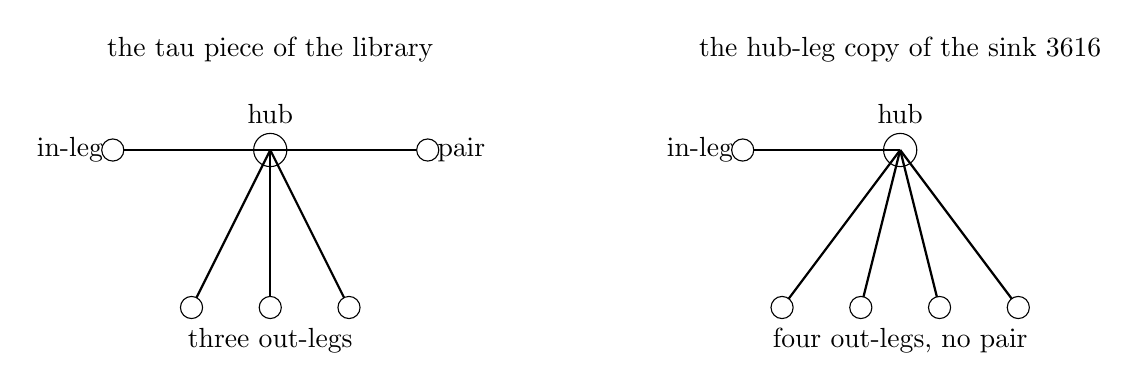
\begin{tikzpicture}[scale=1]
\filldraw[fill=white] (0,0) circle (6pt) node[above=6pt] {hub};
\draw[thick] (0,0) -- (-2,0); \filldraw[fill=white] (-2,0) circle (4pt) node[left] {in-leg};
\foreach \a in {-1,0,1} {\draw[thick] (0,0) -- (\a,-2); \filldraw[fill=white] (\a,-2) circle (4pt);}
\node at (0,-2) [below=4pt] {three out-legs};
\draw[thick] (0,0) -- (2,0); \filldraw[fill=white] (2,0) circle (4pt) node[right] {pair};
\node at (0,1) [above] {the tau piece of the library};
\filldraw[fill=white] (8,0) circle (6pt) node[above=6pt] {hub};
\draw[thick] (8,0) -- (6,0); \filldraw[fill=white] (6,0) circle (4pt) node[left] {in-leg};
\foreach \a in {65mm,75mm,85mm,95mm} {\draw[thick] (8,0) -- (\a,-2); \filldraw[fill=white] (\a,-2) circle (4pt);}
\node at (8,-2) [below=4pt] {four out-legs, no pair};
\node at (8,1) [above] {the hub-leg copy of the sink 3616};
\end{tikzpicture}\caption{A hub-leg piece of the tau web of the library, an in-leg, three out-legs and a pair, beside the hub-leg copy of the first sink of the census, which carries an in-leg and four out-legs and no pair, the first parting.}\end{figure}
\end{chproof}
\section{The dressing-leg chain}\label{mod:VIII-1-D540427-the-dressing-leg-chain}
\begin{chtable}[The dressing-leg chain]\label{box:VIII-1-D540427-the-dressing-leg-chain:1}
This table is conditional on its parent results, the open results, the theorems and the instrument among them read at their grades. The dressing-leg chain at its depth: the thirteen (3,4) results, every one an established result, laid as a derivation graph by text citation with the axiom at the root, every result reached from the root at the graph adopted, thirteen of thirteen, keyed at thirteen of thirteen with no cycle at the graph adopted and at every reading, the ladder and the leg unit located at their results at five of five locators, the (3,4) cell at every result by its pinned token, the slots of the four items beyond this depth kept owed; the first unkeyed result at the hash-only reading, the Higgs-rows result, printed as the face beside; every cell a count of a copy or a citation at a passage, compared with nothing.
\end{chtable}
\chstanding{an instrument}
\chdeps{Definitions 1.1 to 1.6 and Theorems 185.1 to 185.12}{no theorem beyond it at this release}
The results that read the (3,4) genre, the in-leg from a hub to its core qutrit, are gathered into one chain and laid as a directed graph whose edges are citations: a result is the child of another when a line of its own cites the parent, or cites the axiom. Thirteen results stand on the chain, seven theorems and six open results, and the axiom is the root from which every one is reached in at most five steps. The lepton ladder, three to the count, and the hadron ladder, the cap multiplied by a power of three, together with the leg unit twelve are located at the results that spell them. Four slots are kept for items not yet at this depth, and the first result that the stricter hash-only reading cannot key is printed beside.
\begin{chbridge}
A derivation in a formal theory is a directed acyclic graph of results, each proved from foregoing ones and ultimately from the axioms, and a dependency graph of theorems is the usual way such a structure is displayed and checked \cite{Avigad2021,Weinberg1995}. The correspondence is by name.
\end{chbridge}
\begin{chproof}[instrument]
The premises of this derivation are the axiom and the six definitions of chapter~\ref{mod:FRAMEWORK}, the mass unit and the first power of the present chapter, a theorem, and the three generations as attach sites of chapter~\ref{mod:VIII-4-three-generations-as-attach-sites}, a theorem. The chain of premises runs back to the axiom through those chapters, and the longest such chain in this compendium is twelve chapters long.
The table of this chapter is the list of the thirteen results of the chain with their kind, printed in full below with the rule that produced it: every (3,4) result the item and the solution reading name is a node at its established statement. A parent edge is drawn from a node to another whenever a line of the child cites the parent by its text hash within twelve words, or cites the axiom by address, at five readings of the citation. The graph adopted keeps the text-hash and axiom citations alone. The root is the axiom at in-degree zero. The ladder and the leg unit are located by five pinned tokens at their results. The chain is complete when every node is keyed and reached from the root with no cycle.
\begin{center}\begin{adjustbox}{max width=\linewidth}\begin{tabular}{ll}\hline entry & kind \\ \hline the Higgs rows at the hub legs & a theorem \\ the Higgs office at the leg at the quartic and vacuum entries & an open result \\ the lowering dressings as the far-end dressings & a theorem \\ the dressing as the trace over a closed leg & a theorem \\ the geodesic and the tie at the dressing & an open result \\ the geodesic as the passage of the read and the tie as the far-end rule & an open result \\ the Higgs and carrier offices at their sinks & a theorem \\ the dressing as the closed legs of the passage & an open result \\ the (2,4) link read at order two & a theorem \\ the dressing as the Higgs-to-matter leg & an open result \\ hadron spectroscopy at the cap sinks & an open result \\ the chain leptons & a theorem \\ the Higgs quartic as the ratio of offices & a theorem \\ \hline \end{tabular}\end{adjustbox}\end{center}
The thirteen nodes stand at thirteen of thirteen with the (3,4) cell found by its token at every one, the parent edges number fifty-eight over the five readings, six, eleven, ten, nine and twenty-two, and twenty-six at the graph adopted, every node is keyed at thirteen of thirteen, every node is reached from the axiom with the depth five by the longest path, and the graph is acyclic at the graph adopted and at every reading; the ladder is located at two results, the hadron ladder as the cap multiplied by a power of three at the spectroscopy result and the lepton ladder as three to the count at the lowering-dressings result, and the leg unit twelve at three. Printed beside, at the hash-only reading the first unkeyed result is the Higgs-rows result and at the provenance-and-axiom reading the closed-legs result, the older results citing their parents by header and address; the six-genres census names 91 results at the (3,4) genre, 88 of them not nodes of this chain. The chain is an instrument. Its four counter-tests stand at their pinned letters at both engines: a citation planted in memory moves the acyclicity to no with a cycle of five, a result struck whole moves the first unkeyed node, a ladder locator replaced moves the locators found to four of five, and a wrong hash at the gate is excluded; its ten controls read the same, and the chain was reproduced by a second engine built apart from the first, the two equal at every cell.
\end{chproof}
\section{The dressing as the unpassed (3,4) in-legs}\label{mod:VIII-1-D540455-upil-t1}
\begin{chtheorem}[The dressing as the unpassed (3,4) in-legs]\label{box:VIII-1-D540455-upil-t1:1}
The dressing as the unpassed (3,4) in-legs: the dressing of every body, three to the number of (3,4) in-legs its passage leaves unpassed, equals the dressing of the body-alone entry at five of five. The electron, entered at its first dock, passes its one in-leg on the geodesic to its one hub, the count zero and the dressing one; the muon reaches its two hubs tied, every in-leg dressed, the count two and the dressing nine; the tau enters at a (2,2) pair and reaches its first hub through a (2,4) leg, no (3,4) in-leg passed, the count three and the dressing twenty-seven; the proton and the neutron pass the one in-leg on the geodesic to their first hub, the counts two and three and the dressings nine and twenty-seven; the in-legs, the passage and the walk at the hadron entry re-met at every body; the first partings of the passage and Higgs-to-matter-leg entries at the electron re-met by nothing here; a theorem of the passage at the definition adopted, with the control class beside failing at the engine spelling by one representation parting of the second engine at the hadron control letters alone, typed as no fault of substance.
The first face, the dressings one, nine, twenty-seven, nine and twenty-seven equal at five of five, a theorem of the passage, reads yes, the in-legs re-met at five of five, the passage re-met at five of five and the dressings equal at the exponents zero, two, three, two and three; the second face, a body parting, reads no, the first parting none.
\end{chtheorem}
\chstanding{a theorem}
\chdeps{Definitions 1.1 to 1.6 and Theorems 185.1 to 185.12}{no theorem beyond it at this release}
The dressing of a body had been read as a product of far-end dimensions over certain legs, and the foregoing entries parted over which legs, the passage entry and the Higgs-to-matter-leg entry parting first at the electron. This theorem fixes the rule: the read enters a body at the first link of its dock set in link order that is pendant at a qubit, walks the geodesic to the first-reached hubs, dresses every in-leg it reaches at a tie, and the dressing is three to the number of (3,4) in-legs it leaves unpassed, three being the far-end dimension of such a leg. At the electron the one in-leg lies on the geodesic and is passed, so the dressing is one; at the muon the two hubs are reached together and neither in-leg is passed; at the tau the entry is a pair link and the first hub is reached through a (2,4) leg, so all three in-legs stand unpassed. The five dressings so read equal the five of the body-alone entry.
\begin{chbridge}
The physical mass of a charged lepton is its bare mass dressed by its self-interaction, and in the Standard Model the three charged leptons are three copies of one field with three Yukawa couplings and no rule relating them \cite{Weinberg1967,Peskin1995}. The correspondence is by name.
\end{chbridge}
\begin{chproof}[exhaustive census]
The premises of this derivation are the axiom and the six definitions of chapter~\ref{mod:FRAMEWORK}, the mass unit and the first power of the present chapter, a theorem, the body-alone office rule of chapter~\ref{mod:VIII-2-body-alone-office-rule}, a theorem, the lepton ladder as hub assemblies of chapter~\ref{mod:V-10-lepton-ladder-as-hub-assemblies}, a theorem, and the three generations as attach sites of chapter~\ref{mod:VIII-4-three-generations-as-attach-sites}, a theorem. The chain of premises runs back to the axiom through those chapters, and the longest such chain in this compendium is twelve chapters long.
By exhaustive enumeration of the thirteen (3,4) in-legs of the five bodies, the in-leg a (3,4) link at a hub, a site of dimension four at degree three or more, its far end the qutrit: the electron has the one in-leg $HA$. The muon has $HA$ and $H_{2}B$. The tau has $HA$, $H_{2}B$ and $H_{3}C$. The proton has $s_{3}s_{7}$, $s_{4}s_{7}$ and $s_{5}s_{7}$ at the hub $s_{7}$. The neutron has $HQ_{1}$, $HQ_{2}$, $HQ_{3}$ and $Q_{2}F$ at the hubs $H$ and $F$. Every one stands at the leg register twelve. The property tested at each in-leg is whether the passage, entered at the first dock-set link in link order pendant at a qubit, stopping at the first-reached hubs with every in-leg dressed at a tie, passes it; the counts by body are the unpassed in-legs zero, two, three, two and three, and the dressings
\begin{equation} 3^{0} = 1, \qquad 3^{2} = 9, \qquad 3^{3} = 27, \qquad 3^{2} = 9, \qquad 3^{3} = 27, \end{equation}
equal to the dressings of the body-alone entry at five of five, the first parting none, and equal to the passage, geodesic-and-tie, closed-legs and Higgs-to-matter-leg cells at twenty of twenty. The smallest case worked is the electron: entered at the pendant qubit $w_{1}$, its steps run $w_{1}$ at zero, $B$ at one, $A$ and $C$ at two, $H$ and $w_{2}$ at three, the stop at $H$ at the third step, the geodesic through $AB$, $HA$ and $Bw_{1}$, so the one in-leg $HA$ is passed and the dressing is one. Beside, the sixty-four words of the fixed library at the same walk give the exponent defined at nineteen, the dressings one at nine, nine at seven and twenty-seven at three, no dock at thirty-eight and no hub at seven, printed and deciding nothing.
The counter-tests alter the construction singly and read what moves. Reversing the tie passes both in-legs of the muon and moves its dressing to one and the first body to the muon. Entering at the last dock moves the stops and the passed legs with the dressings moving at no body. Taking the base at the hub dimension moves the dressings to one, sixteen, sixty-four, sixteen and sixty-four. Striking the axiom text unmeets the gate. Each alteration moves the cells it names, four of four. The result was reproduced by an independent route, two engines built apart, a map route against the second route, equal at every cell of the item; the controls read the same at seventeen of twenty at both engines and twenty of twenty at the first, the three apart being one representation parting of the second engine at the hadron control letters, a sorted string of name-and-step pairs against the site names, moving no cell and typed as no fault of substance. The machine-checked package named at the reproducibility appendix certifies the statements of this chapter under the definitions of this compendium and proves no theorem of the literature.
\chcert{13}
\end{chproof}
\section{The five mass-unit spellings at the (2,2) office}\label{mod:VIII-1-D542746-the-five-mass-unit-spellings-at-the-two-two-office}
\begin{chtable}[The five mass-unit spellings at the (2,2) office]\label{box:VIII-1-D542746-the-five-mass-unit-spellings-at-the-two-two-office:1}
This table is conditional on its parent results, the open results and the theorem read at their grades. The five mass-unit spellings at the (2,2) office at this depth: the five elements, one, thirty-six, sixteen, sixty-seven and sixty-seven, transcribed from the five mass-unit open results against the office of one serial (2,2) link at the seven chains at the reading adopted, equal at zero of thirty-five cells, the first face one element no and the second face the spellings that part, every one of the five at every one of the seven chains, printed with the spellings beside and the readings beside; the controls the same at fourteen of fourteen, the counter-tests at their pinned letters four of four.
\end{chtable}
\chstanding{an instrument}
\chdeps{Definitions 1.1 to 1.6 and Theorems 185.1 to 185.12}{no theorem beyond it at this release}
Five foregoing open results each spelled the mass unit as a cell, the tick at the one tick as one, the whole rung register as thirty-six, the common-support register of the electron dock as sixteen, the dock-struck unit as sixty-seven, and the first power at the probe hub leg as sixty-seven. A subsequent theorem read the tick as the office of one serial (2,2) link at each chain, an element of the field with a root-two part. This table sets the five spellings against that office at the seven chains and finds that none equals it anywhere, so no one of the five spellings is the office and the mass unit stays a question of which cell is meant; the table feeds the unit chapter.
\begin{chbridge}
The unit of mass in a physical theory is a convention fixed by a chosen standard, and in particle physics the electron mass or the electronvolt serves, every other mass a pure number in that unit \cite{Weinberg1995,Jackson1998}. The correspondence is by name.
\end{chbridge}
\begin{chproof}[instrument]
The premises of this derivation are the axiom and the six definitions of chapter~\ref{mod:FRAMEWORK}, the mass unit and the first power of the present chapter, a theorem, and the tick scale as a coupling scale of chapter~\ref{mod:X-10-tick-scale-as-a-coupling-scale}, a theorem. The chain of premises runs back to the axiom through those chapters, and the longest such chain in this compendium is twelve chapters long.
The table of this chapter is printed in full below with the rule that produced it: each of the five mass-unit open results is transcribed at its cell from its copy, the element it spells as the unit at its own face; the office of one serial (2,2) link is read as the tick entry carries it at every chain at the reading adopted, the increment read as an office; each spelling is compared with the office at each of the seven chains and read equal or parting, exactly.
\begin{center}\begin{adjustbox}{max width=\linewidth}\begin{tabular}{llll}\hline spelling & the open result it comes from & element & against the office at the seven chains \\ \hline the tick at the one tick & the mass unit at the one tick & $1$ & parts at seven of seven \\ the whole rung register & the mass unit as the rung register & $36$ & parts at seven of seven \\ the common-support register of the electron dock & the mass unit as the office at the common support & $16$ & parts at seven of seven \\ the dock-struck unit & the mass-unit spelling as a theorem & $67$ & parts at seven of seven \\ the first power at the probe hub leg & the mass-unit spelling at the probe hub leg & $67$ & parts at seven of seven \\ \hline \end{tabular}\end{adjustbox}\end{center}
The office of one serial (2,2) link at the seven chains is $\tfrac{536569}{972} + \tfrac{25}{1458}\sqrt{2}$ at the electron, $\tfrac{847609}{12} + \tfrac{25}{18}\sqrt{2}$ at the muon, $\tfrac{3475947}{4} + \tfrac{25}{2}\sqrt{2}$ at the tau, zero at the proton and at the neutron, $\tfrac{202201}{972} + \tfrac{25}{1458}\sqrt{2}$ at the photon word and $\tfrac{917593}{12} + \tfrac{25}{18}\sqrt{2}$ at the body of the universe web, so the first parting of every spelling is at the electron chain, one, thirty-six, sixteen, sixty-seven and sixty-seven against $\tfrac{536569}{972} + \tfrac{25}{1458}\sqrt{2}$; the thirteen spellings beside and the three readings beside give 648 cells, equal at none. The table is an instrument. Its four counter-tests stand at their pinned letters at both engines: a spelling replaced by the office in memory moves two cells to equal, the office at one chain replaced by the rung register moves twelve cells, the office filled with the tick at every chain and reading moves 216 cells, and a wrong hash at the gate is excluded; its fourteen controls read the same, and the table was reproduced by a second engine built apart from the first, the two equal at every cell.
\end{chproof}
\section{The six dressings at the six genres}\label{mod:VIII-1-D542965-w-sxdr}
\begin{chwall}[The six dressings at the six genres]\label{box:VIII-1-D542965-w-sxdr:1}
The alpha machinery run at the six genres refuses at no genre and prints one exact element of the ring at every genre with a qubit far end and two exact elements, one at each spelling of the closure sector, at every genre beyond it, the first parting the (3,3) genre: the pole is printed at every genre, the center acting at the mixed genres and not at the homogeneous genres, the unit functional holding the one-link identity at 48 of 48 paths at every genre, the closed reads empty at every open form, the pole at the order one at (2,2) and (2,3) and at the order two at the four dark genres, equal to the readability entry at six of six; the dressing at the package spelling is $\tfrac{30 + 30\sqrt{2}}{2304}$, $\tfrac{79 + 48\sqrt{2} + 42\sqrt{3} + 3\sqrt{6}}{31104}$, $\tfrac{450 + 96\sqrt{2}}{184320}$, $\tfrac{208 + 200\sqrt{3}}{419904}$, $\tfrac{685 + 256\sqrt{3}}{2488320}$ and $\tfrac{2100}{14745600}$, and at the count-law spelling $\tfrac{268 + 200\sqrt{3}}{419904}$, $\tfrac{685 + 296\sqrt{3}}{2488320}$ and $\tfrac{2460}{14745600}$ at the three genres where the spellings part, the closure sector 8 against 28, 8 against 28 and 15 against 105; the dressing per unit equals the dressing at every genre at both readings; the six elements equal the established columns at (2,2) and (2,3) and differ at (2,4), (3,3), (3,4) and (4,4), the first differing column (2,4); both faces printed, no observed value anywhere, compared with nothing.
The first face, six exact elements of one ring printed, reads no, the machinery printing one element at the three genres with a qubit far end and two at the three genres beyond, the genres at one element three of six; the second face, the genre at which the machinery refuses named, reads no, no step refusing at any genre, the first refusing genre none. Open is the closure sector at a qutrit or ququart far end: the polynomial spelling of the package counts the closure records as the commutators of the three far-end letters of a qubit, three at every qubit far end, and the count law of the six genres counts the pairs of the far-end letters, so the two coincide wherever the far end is a qubit and part wherever it is not, first at the (3,3) genre, and this result lays neither spelling.
\end{chwall}
\chstanding{an open result}
\chdeps{Definitions 1.1 to 1.6 and Theorems 185.1 to 185.12}{no theorem beyond it at this release}
The machinery that derives the fine-structure constant at the one (2,3) link, the identification algebra with its center, the Ward read at the unit functional, the census of the records of two reads with their weights, the register and the unit, is run unchanged at each of the six genres of the link. At every genre every step goes through: the algebra closes with a one-line center, the unit functional holds the identity, every weight is a root in the ring and the register is positive. The one ambiguity is the closure sector of the census, which the package spells by a polynomial in the far-end dimension and the count law of the six genres spells by the pairs of the far-end letters; at a qubit far end both give three and the dressing is one element, at a qutrit or ququart far end they give eight against twenty-eight or fifteen against one hundred and five and the dressing is one of two elements. The open result prints both at the three parting genres and lays neither.
\begin{chbridge}
The coupling of a gauge theory is one number at each gauge group, the fine-structure constant for the abelian group and the strong coupling for the color group, and the running of each is governed by its own beta function with a universal form across the groups \cite{Peskin1995,Gross1973}. The correspondence is by name.
\end{chbridge}
\begin{chproof}[finite computation with its census and its exact part]
The premises of this derivation are the axiom and the six definitions of chapter~\ref{mod:FRAMEWORK}, the mass unit and the first power of the present chapter, a theorem, the link and its six genres of chapter~\ref{mod:I-2-link-and-its-six-genres}, a theorem, the fine-structure constant at the one link of chapter~\ref{mod:V-1-fine-structure-constant-at-the-one-link}, a theorem, and the Ward functional and the dressing per unit of that chapter, an open result. The chain of premises runs back to the axiom through those chapters, and the longest such chain in this compendium is twelve chapters long.
\textit{The objects.} The six genres of the link are (2,2), (2,3), (2,4), (3,3), (3,4) and (4,4) at their end dimensions, each with its pair ket on the common support of two, two, two, three, three and four directions and its identification algebra of 7, 12, 19, 17, 24 and 31 elements with the brackets closed at 49, 144, 361, 289, 576 and 961 and the center one line at the primitive diagonal, $1,1,-1,-1$ at (2,2), $3,3,-2,-2,-2$ at (2,3) and $2,2,-1,-1,-1,-1$ at (2,4) among them. The figure draws the six links.
\textit{The procedure.} At each genre, re-derive the algebra and its center and read the center on the pair ket, acting or not. Re-implement the Ward read at the eight orderings and forty-eight paths and test the unit functional. Census the records of two reads by the polynomials of the package at the traceless dimensions of the two ends, three and three at (2,2), eight and three at (2,3), fifteen and three at (2,4), eight and eight at (3,3), fifteen and eight at (3,4) and fifteen and fifteen at (4,4), in the odd, mixed-even and same-even sectors, and the closure sector at both spellings, the polynomial of the package and the count law of the six genres by locator. Weight the records by the exchanges and sum over the register, the cut register multiplied by the whole register squared, for the dressing. Read the unit at the pair ket and per record and divide for the dressing per unit. Compare the six elements with the established columns.
\textit{The exact part and the smallest instance.} The records number 57, 172, 417, 392 against 412, 777 against 797 and 1365 against 1455 at the six genres, the closure sector at the two spellings 3, 3, 3, 8 against 28, 8 against 28 and 15 against 105. At the first parting genre (3,3) the register is $419904 = 64\cdot 81\cdot 81$ and the two dressings read
\begin{equation} D_{33}^{\mathrm{package}} = \frac{208 + 200\sqrt{3}}{419904}, \qquad D_{33}^{\mathrm{count\ law}} = \frac{268 + 200\sqrt{3}}{419904}, \end{equation}
the difference the sixty closure records of the count law beyond the eight of the polynomial at the weight one; at (3,4) the two read $\tfrac{685 + 256\sqrt{3}}{2488320}$ and $\tfrac{685 + 296\sqrt{3}}{2488320}$ and at (4,4) $\tfrac{2100}{14745600}$ and $\tfrac{2460}{14745600}$, while at (2,2), (2,3) and (2,4) the one element is $\tfrac{30 + 30\sqrt{2}}{2304}$, $\tfrac{79 + 48\sqrt{2} + 42\sqrt{3} + 3\sqrt{6}}{31104}$ and $\tfrac{450 + 96\sqrt{2}}{184320}$. The unit functional at the pair ket reads one, five sixths, three quarters, two thirds, seven twelfths and one half at the six genres and two per record at the sector level, and the dressing per unit equals the dressing at every genre at both readings. The pole stands at the order one at (2,2) and (2,3) and at the order two at the four dark genres, equal to the readability entry at six of six.
\textit{The census.} By exhaustive enumeration of the six genres at every step of the machinery: the property tested is whether a step refuses, the algebra not closing or its center not one line, the unit functional not holding, a weight outside the ring, the register not positive or the unit zero; the count of refusing genres is none, and the count of genres printed at one element is three of six, the first parting (3,3). The six elements equal the established columns at (2,2) and (2,3) and differ at (2,4), (3,3), (3,4) and (4,4), the first differing column (2,4).
\textit{The check.} The counter-tests alter the construction singly and read what moves. Striking the center moves the central element to zero at every genre and the machinery refuses at (2,2) at the algebra step. Swapping the ends negates the pair scalar at the mixed genres. Reading a dimension-five end refuses at the Ward read, an end outside the alphabet and a weight outside the ring. Reading the count at the record level refuses at every genre but (2,3). Striking the text unmeets the gate. Each alteration moves the cells it names, five of five. The result was reproduced by an independent route, two engines built apart, a map-and-fraction route against the second route, equal at every cell, with the fourteen controls the same.
\chcert{6}
\begin{figure}[h]\centering\begin{adjustbox}{max width=\linewidth}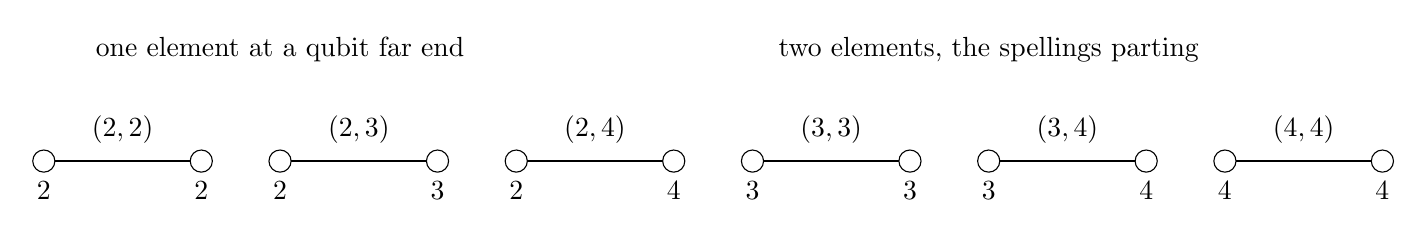
\begin{tikzpicture}[scale=1]
\foreach \x/\a/\b/\g in {0/2/2/{(2,2)}, 3/2/3/{(2,3)}, 6/2/4/{(2,4)}, 9/3/3/{(3,3)}, 12/3/4/{(3,4)}, 15/4/4/{(4,4)}} {\draw[thick] (\x,0) -- (\x+2,0); \filldraw[fill=white] (\x,0) circle (4pt) node[below=4pt] {$\a$}; \filldraw[fill=white] (\x+2,0) circle (4pt) node[below=4pt] {$\b$}; \node at (\x+1,0) [above=3pt] {$\g$};}
\node at (3,1) [above=4pt] {one element at a qubit far end};
\node at (12,1) [above=4pt] {two elements, the spellings parting};
\end{tikzpicture}\end{adjustbox}\caption{The six genres of the link with their end dimensions; at the three with a qubit far end the two spellings of the closure sector coincide and the dressing is one element, at the three beyond they part.}\end{figure}
\end{chproof}
\section{The office as a formula in the membership counts}\label{mod:VIII-1-D543206-w-ofmc}
\begin{chwall}[The office as a formula in the membership counts]\label{box:VIII-1-D543206-w-ofmc:1}
The formula in the six counts misses an established office, the first the W word: with $n$ the membership vector over the six genres, $s$ the struck vector, $k$ the dressing exponent, $m_{g}$ the weight of the genre and $G_{2,g}$ its second-order readout at the larger dimension, the formula $F(n; s, k) = 9^{k}\big\{\big(\sum_{g} m_{g}(n_{g} - s_{g})\big)^{2} + \sum_{g\ \mathrm{dark}} (n_{g} - s_{g})\, m_{g}^{2}\, G_{2,g}^{2}\big\}$ with $G_{2,g}$ per genre at the larger dimension is met at nineteen of twenty-six reads and missed first at the W word, the parting the closure at the (2,4) genre, $\tfrac{6137}{3645000} + \tfrac{4}{6075}\sqrt{2}$ against $\tfrac{10241}{3645000} + \tfrac{98}{50625}\sqrt{2}$; at the slot reading of the readout, per link at the end of larger degree and no function of the counts alone, the formula meets twenty-two of twenty-six; the first face unmet at the reading adopted, the second face met with the first body named with both cells; every cell an exact element of the field of root two and root three compared with nothing.
The first face, one formula in the six counts meeting every established office so that the spectrum is the membership table multiplied by the cell dressings and the hadron, lepton and cross-core open results become instances of one formula with their partings located at a count, reads no, the formula met at nineteen of twenty-six; the second face, the first body the formula misses named with both cells, reads yes at the W word, the parting located at the (2,4) closure. Open is the closure as a function of the counts: the per-genre closure of the formula at the larger-dimension slot parts from the per-link closure at the slot of larger degree wherever a dark link is slotted at its smaller end, and the formula at the slot reading meets that body.
\end{chwall}
\chstanding{an open result}
\chdeps{Definitions 1.1 to 1.6 and Theorems 185.1 to 185.12}{no theorem beyond it at this release}
The body-alone rule reads the office of a body link by link, the first power as a weighted count of its unstruck links, the closure as a sum over its dark links of the squared act multiplied by the second-order readout. This entry asks whether the office is a closed form in six numbers alone, the membership counts of the links by genre, with the struck links and the dressing exponent as the two indices. For nineteen of the twenty-six reads it is. It fails first at the W word of the fixed library, whose two (2,4) legs are slotted at their qubit end, so that the per-link readout at the slot of larger degree differs from the readout the formula assigns to the (2,4) genre at its larger dimension; the first power 28 and its square 784 agree, the closures do not. The parting is a matter of the slot of a dark link and not of the counts, and the three dressing open results of the chapter are re-read as instances of the formula at a count.
\begin{chbridge}
A mass formula in particle physics expresses the masses of a multiplet in terms of a few quantum numbers and parameters, the Gell-Mann and Okubo formula for the baryon octet the standard example, with the residual splittings attributed to interactions the formula omits \cite{GellMann1962,Okubo1962}. The correspondence is by name.
\end{chbridge}
\begin{chproof}[finite computation with its census]
The premises of this derivation are the axiom and the six definitions of chapter~\ref{mod:FRAMEWORK}, the mass unit and the first power of the present chapter, a theorem, the body-alone office rule of chapter~\ref{mod:VIII-2-body-alone-office-rule}, a theorem, the Higgs and carrier offices at their sinks of chapter~\ref{mod:VI-10-higgs-the-closed-hub-read-its-rows-its-mass-and-its-exponent}, a theorem, and the dressing as the unpassed (3,4) in-legs of the present chapter, a theorem. The chain of premises runs back to the axiom through those chapters, and the longest such chain in this compendium is twelve chapters long.
\textit{The procedure.} The input objects are the twenty-six reads, eight of the Higgs-and-carrier-offices entry at the measure-struck reading, seven of the body-alone entry at the segment reading, six of the tau-web entry, two tau-form sinks of the lepton-sink entry and three of the cross-core entry, each with its office under the rule re-met at every link, every link at its weight, the product of the end dimensions, the dock set struck, the dressing the far-end product over the in-legs at hubs, and the closure at a dark link the square of the act multiplied by the second-order readout at its slot. For each read form the membership vector $n$ over the genres (2,2), (2,3), (2,4), (3,3), (3,4) and (4,4), the struck vector $s$ and the exponent $k$, and evaluate the formula with the weights $m_{g}$ of 4, 6, 8, 9, 12 and 16 and the readouts at the larger dimension, $\tfrac{5}{216} + \tfrac{5}{216}\sqrt{2}$ at (2,2), $\tfrac{1}{288} + \tfrac{1}{1350}\sqrt{2}$ at (2,4), $\tfrac{67}{82944} + \tfrac{25}{41472}\sqrt{3}$ at (3,3), $\tfrac{137}{414720} + \tfrac{37}{259200}\sqrt{3}$ at (3,4) and $\tfrac{41}{216000}$ at (4,4), the (2,3) genre outside the dark set; compare with the office and name the first read missed.
\textit{The smallest instance.} The W word carries the membership vector $(0, 2, 2, 0, 0, 0)$, the struck vector zero and the exponent zero, so its first power is $6\cdot 2 + 8\cdot 2 = 28$ with the square $784$, and the closure term of the formula at its two dark (2,4) links is
\begin{equation} 2\cdot 8^{2}\cdot\Big(\tfrac{1}{288} + \tfrac{1}{1350}\sqrt{2}\Big)^{2} = \tfrac{6137}{3645000} + \tfrac{4}{6075}\sqrt{2}, \qquad F = 784 + \tfrac{6137}{3645000} + \tfrac{4}{6075}\sqrt{2} = \tfrac{2857686137}{3645000} + \tfrac{4}{6075}\sqrt{2}, \end{equation}
against the office $\tfrac{2857690241}{3645000} + \tfrac{98}{50625}\sqrt{2}$, whose closure $\tfrac{10241}{3645000} + \tfrac{98}{50625}\sqrt{2}$ is read per link at the slot of larger degree, the qubit end of each leg; the parting is located at the (2,4) closure and at no count.
\textit{The census.} By exhaustive enumeration of the twenty-six reads at the reading adopted, the struck vector and the exponent of the read with the readout per genre at the larger dimension: the property tested is equality of the formula with the office; the counts are met at nineteen of twenty-six, missed at seven, the W word, the Z word, the proton, the neutron through the deuteron, the strike-rule neutron, the one-link electron and the tau sink; printed beside, at the slot reading of the readout the formula meets twenty-two of twenty-six and at the pure-count reading seven of twenty-six; the 179 per-link readout cells of the reads are re-met by the count law at 179 of 179; and the three dressing open results of the chapter are re-read as instances of the formula at a count.
\textit{The check.} The counter-tests alter the construction singly and read what moves. Incrementing the struck vector at the (2,2) genre moves every read carrying an unstruck pair. Adding one (4,4) link to every membership vector moves every read and the first body missed to the Higgs word. Dropping the closure moves every read with a nonzero closure. Reading a word of the library with no office, the gluon word, holds at its cells with the formula and the rule printed and compared with nothing. Striking the gate exits at both engines. Each alteration moves the cells it names, five of five. The result was reproduced by an independent route, two engines built apart, the explicit record-space route against the second route, equal at every cell; the controls read the same at fourteen of fifteen at the pinned grammar, the fifteenth mis-posed at two reads carrying no census row and re-read holding at the census-keyed reads at twenty-four of twenty-four.
\chcert{26}
\end{chproof}
\par\medskip\noindent{\itshape The unit fixed, the next chapter says which office a body reads alone.}\label{narr:close:8-1}\par
\section{The body-alone office rule}\label{mod:VIII-2-body-alone-office-rule}
\chdesig{10-2}{8-2}{VIII-2-body-alone-office-rule}{VIII-2-body-alone-office-rule}
\label{narr:open:8-2}Theorem~195.1 is the body-alone office rule, a theorem resting on the records, the saturation and the mass unit, and the quark and carrier offices of Parts VIII and IX rest on it.
\begin{chtheorem}[The body-alone office rule]\label{box:VIII-2-body-alone-office-rule:1}
The office of every body at its own sink is defined as an exact nonzero element of the field at the five bodies: its pair part equals the first power squared of the segment theorem by the two-read identity, and its closure part is an exact cell, positive at the three leptons and zero at the proton and at the neutron through the deuteron.
\end{chtheorem}
\chstanding{theorem}
\chdeps{Definitions 1.1 to 1.6, Theorems 18.1 to 18.4 and Open results 18.5 and 18.6, Theorems 185.1 to 185.12 and Open results 245.1 and 245.2, Theorem 245.3, Open results 245.4 to 245.8 and Theorem 245.9}{the theorems of Chapters 1-1, 1-3, 1-5, 4-6, 5-3, 5-8, 5-8f, 6-2, 6-6, 9-7, 11-1, 12-1}
The reading adopted takes the act read of every link from the segment theorem, the dark set as every link of a genre other than the read genre, and the closure at a dark link as the square of its act read multiplied by the grid factor. The readings of the grid meet at every segment reading. The rule itself is the chapter. A body belongs to the force of its defining read, and the quark offices and the Higgs and carrier offices of their own chapters take this rule as their derivation.
\begin{chbridge}
The rest mass of a body is the invariant of its four-momentum, in the Standard Model a parameter of the Lagrangian for each field set by its coupling to the Higgs field and fixed by nothing within the theory, and the Born rule reads the probability of an outcome as the squared modulus of the amplitude of the transition \cite{Born1926,Dirac1928,Weinberg1967}. The correspondence is by name.
\end{chbridge}
\begin{chproof}[finite computation with its exact part]
\textit{The premises.} The axiom and the six definitions of Section~\ref{mod:FRAMEWORK}, definitions. The Born count and the gain lemma of Section~\ref{mod:I-3-records-reads-and-the-born-count-the-gain-lemma}, a theorem. The sinks of the saturation of Section~\ref{mod:I-5-saturation-in-one-figure-seeds-waves-termination-sinks}, a theorem. The mass unit and the first power of Section~\ref{mod:VIII-1-mass-unit-and-the-first-power}, a theorem. The chain from the axiom to this result is six chapters deep.

\textit{The exact part: the office of one body.} A body is read at its own sink and nowhere else. Its web has sites and links, each link of a genre given by the two end dimensions. The read enters at a dock of the read genre, the (2,3) genre, and the segment theorem assigns to every link an act read. From the act reads of the links, by summation, we obtain the first power of the body,
\begin{equation}
S_1=\sum_{\ell} a_\ell ,
\end{equation}
the sum running over the links of the web. From the first power, by the two-read identity (the sum over the ordered pairs of links of the product of their act reads equals the square of the sum), we obtain the pair part,
\begin{equation}
\mathrm{pair}=\sum_{\ell,\ell'} a_\ell a_{\ell'}=S_1^{2}.
\end{equation}
From the dark set, every link of a genre other than (2,3), and the grid factor $G_2$ of the count law at the six genres, by the closure rule of this chapter (a dark link closes at the square of its act read multiplied by the grid factor, a link read at nothing closing at nothing), we obtain the closure part,
\begin{equation}
\mathrm{closure}=\sum_{\ell\ \mathrm{dark}} a_\ell^{2}\,G_2 ,
\end{equation}
an element of the ring with basis one, root two, root three and root six. From the pair part and the closure part, by addition, we obtain the office of the body at its own sink, $\mathrm{office}=\mathrm{pair}+\mathrm{closure}$.

\textit{The smallest instance.} The one-link electron web is one (2,3) link. Its act read is the unit, $S_1=67$. The dark set is empty, so by the three displays
\begin{equation}
\mathrm{pair}=67^{2}=4489,\qquad \mathrm{closure}=0,\qquad \mathrm{office}=4489 .
\end{equation}

\textit{The finite computation at the five bodies.} The input objects are the five webs. The electron stands at its two-dock web, drawn at the figure, with ten links, the measure 79 and the dock set 12 at its two (2,3) docks. The muon stands at its web of fifteen links, the measure 117 and the dock set 10. The tau stands at its web of twenty links, the measure 155 and the dock set 8. The proton stands at the sink of the bound-respecting reading with nine links, the measure 81 and the dock set 18, its entered link capped at the cap of its genre. The neutron through the deuteron stands at the typing adopted with twenty-eight links, the measure 219 and the dock set 36, its entered link capped. The enumeration rule is the one procedure of the exact part applied to each web with no body-specific term. The test applied to each body is whether the pair part equals the first power squared and whether the closure part is an exact element of the ring. The aggregation is the office. The first powers at the natural checkpoint are
\begin{equation}
S_1=67,\ 963,\ 3969,\ 2871,\ 2871
\end{equation}
at the electron, the muon, the tau, the proton and the neutron through the deuteron, and the pair parts are their squares,
\begin{equation}
\mathrm{pair}=4489,\ 927\,369,\ 15\,752\,961,\ 8\,242\,641,\ 8\,242\,641 ,
\end{equation}
the two-read identity holding at every one of the 760 cells of the grid of readings. The closure parts at the three leptons are
\begin{align}
\mathrm{closure}_{e}&=\tfrac{13\,708\,610\,839}{477\,757\,440\,000}+\tfrac{661}{36\,450}\sqrt{2}+\tfrac{5\,977\,541}{23\,887\,872\,000}\sqrt{3}\quad\text{at eight dark links},\\
\mathrm{closure}_{\mu}&=\tfrac{27\,214\,907\,303}{5\,898\,240\,000}+\tfrac{661}{225}\sqrt{2}+\tfrac{6\,301\,957}{294\,912\,000}\sqrt{3}\quad\text{at fourteen dark links},\\
\mathrm{closure}_{\tau}&=\tfrac{40\,721\,203\,767}{655\,360\,000}+\tfrac{1983}{50}\sqrt{2}+\tfrac{6\,626\,373}{32\,768\,000}\sqrt{3}\quad\text{at twenty dark links},
\end{align}
each positive, and at the proton and at the neutron through the deuteron the closure part is zero, every dark link beyond the first cap being read at nothing (six dark links at the proton, twenty-two at the neutron through the deuteron). From the pair parts and the closure parts, by addition, we obtain the offices
\begin{align}
\mathrm{office}_{e}&=\tfrac{2\,144\,666\,856\,770\,839}{477\,757\,440\,000}+\tfrac{661}{36\,450}\sqrt{2}+\tfrac{5\,977\,541}{23\,887\,872\,000}\sqrt{3},\\
\mathrm{office}_{\mu}&=\tfrac{5\,469\,872\,145\,467\,303}{5\,898\,240\,000}+\tfrac{661}{225}\sqrt{2}+\tfrac{6\,301\,957}{294\,912\,000}\sqrt{3},\\
\mathrm{office}_{\tau}&=\tfrac{10\,323\,901\,242\,163\,767}{655\,360\,000}+\tfrac{1983}{50}\sqrt{2}+\tfrac{6\,626\,373}{32\,768\,000}\sqrt{3},\\
\mathrm{office}_{p}&=\mathrm{office}_{n}=8\,242\,641 ,
\end{align}
every one an exact nonzero element of the field, which is the statement. The ratio of the proton office to the one-link electron office is the exact cell $8\,242\,641/4489$, the Born-square ratio of the neutron result re-met.

\textit{The check.} Striking the closure records at the muon moves the muon office. Reading a dark link at first order, so that the dark set of the electron is empty, moves the electron closure. Leaving the dock of the electron unstruck moves the electron pair part away from the first power squared. Lifting the cap at the proton moves the proton pair part away from the first power squared. Each alteration moves the cell it names and nothing else. The result was reproduced by an independent route, a map-and-fraction route and an array-scan big-integer route agreeing at every deciding cell at both runs, with the two-read identity as the control at every cell of the grid. The derivation follows the spelling of the mass result and of the neutron result, which it cites as its precedents.
\chcert{80}
\end{chproof}
\begin{figure}[H]\centering
\begin{tikzpicture}[x=0.52pt,y=-0.52pt,baseline]
\clip (0,0) rectangle (900,540);
\fill[white] (0,0) rectangle (900,540);
\node[anchor=base west,inner sep=0pt,text=black,font=\fontsize{6.76}{8.112}\selectfont\ttfamily] at (12,22) {atlas body-alone:E1: one-link-web};
\node[anchor=base west,inner sep=0pt,text=black,font=\fontsize{6.24}{7.488}\selectfont\ttfamily] at (12,42) {membership 22:0;23:1;24:0;33:0;34:0;44:0; cells (2,3); links 1; sites 2; measure 6; census at the census};
\node[anchor=base west,inner sep=0pt,text=black,font=\fontsize{5.72}{6.864}\selectfont\ttfamily] at (12,62) {recorded office body-alone:E1:segment/R1/weight:E1=4489\textbar{}0\textbar{}0\textbar{}0; standing census:instrument;body-alone:theorem;formula:open result; board none};
\draw[draw=black,line width=1.04pt,dash pattern=on 1.04pt off 1.56pt] (100,470) .. controls (130,450) and (160,450) .. (190,470);
\node[anchor=base,inner sep=0pt,text=black,font=\fontsize{5.72}{6.864}\selectfont\ttfamily] at (145,451) {(2,3)};
\filldraw[fill={rgb,255:red,244;green,192;blue,192},draw=black,line width=0.52pt] (100,470) circle (14);
\node[anchor=base,inner sep=0pt,text=black,font=\fontsize{6.24}{7.488}\selectfont\ttfamily] at (100,475) {0};
\node[anchor=base,inner sep=0pt,text=black,font=\fontsize{5.72}{6.864}\selectfont\ttfamily] at (100,500) {x2};
\filldraw[fill={rgb,255:red,244;green,192;blue,192},draw=black,line width=0.52pt] (190,470) circle (14);
\node[anchor=base,inner sep=0pt,text=black,font=\fontsize{6.24}{7.488}\selectfont\ttfamily] at (190,475) {0};
\node[anchor=base,inner sep=0pt,text=black,font=\fontsize{5.72}{6.864}\selectfont\ttfamily] at (190,500) {x3};
\node[anchor=base west,inner sep=0pt,text=black,font=\fontsize{5.72}{6.864}\selectfont\ttfamily] at (12,510) {the sites labelled by register (2 the qubit, white; 3 the qutrit, grey; 4 the ququart, dark); the links labelled by cell (p,q); a long dash an open dark link of the neutron row; a short dash a docked link at the rule R1};
\end{tikzpicture}
\caption{\texttt{one-link-web}, one link web: 2 sites, 1 links, the measure 6; the links at the cells (2,3); the membership 22:0; 23:1; 24:0; 33:0; 34:0; 44:0; 1 docked links at the rule R1 (x3-x2); at the census of the six cells; 2 sites at the fourth band with the register unresolved by the genre alone, the drawing gloss not drawn at them as the compendium prints it. Drawn at the anatomy atlas as its web, the sites labeled by register and the links by cell, from the the body-alone office rule.}\label{fig:VIII-2-D537322-one-link-web-1d74cd}
\begin{center}\footnotesize\begin{adjustbox}{max width=\linewidth}\begin{tabular}{p{0.26\textwidth}p{0.68\textwidth}}\toprule
recorded office (the slot-count row) & the read O-E1 of the formula row: the first power 67; the office \texttt{4489\textbar{}0\textbar{}0\textbar{}0}; against the formula with the slot count equal; the slot total 0; dark links 0; hubs none; dressing 1 \\
mass register (the mass-register row) & the read BE1: the class within the qubit and the qutrit; the first power 0; the office \texttt{0\textbar{}0\textbar{}0\textbar{}0}; zero; met yes; hubs none; in-legs none; dressing 1; ports x3-x2 \\
\bottomrule\end{tabular}\end{adjustbox}\end{center}
\end{figure}
\begin{figure}[H]\centering
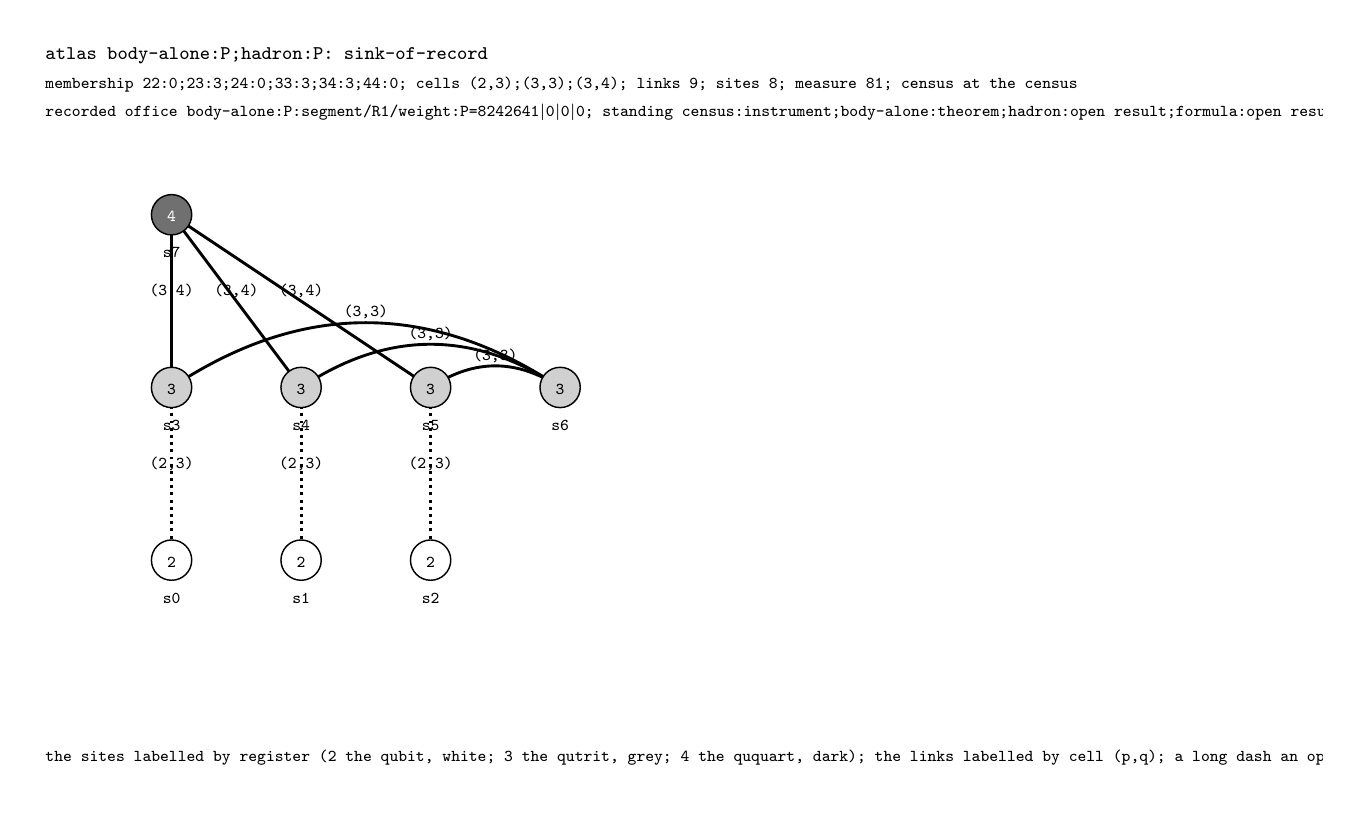
\begin{tikzpicture}[x=0.52pt,y=-0.52pt,baseline]
\clip (0,0) rectangle (900,540);
\fill[white] (0,0) rectangle (900,540);
\node[anchor=base west,inner sep=0pt,text=black,font=\fontsize{6.76}{8.112}\selectfont\ttfamily] at (12,22) {atlas body-alone:P;hadron:P: sink-of-record};
\node[anchor=base west,inner sep=0pt,text=black,font=\fontsize{6.24}{7.488}\selectfont\ttfamily] at (12,42) {membership 22:0;23:3;24:0;33:3;34:3;44:0; cells (2,3);(3,3);(3,4); links 9; sites 8; measure 81; census at the census};
\node[anchor=base west,inner sep=0pt,text=black,font=\fontsize{5.72}{6.864}\selectfont\ttfamily] at (12,62) {recorded office body-alone:P:segment/R1/weight:P=8242641\textbar{}0\textbar{}0\textbar{}0; standing census:instrument;body-alone:theorem;hadron:open result;formula:open result; board proton};
\draw[draw=black,line width=1.04pt,dash pattern=on 1.04pt off 1.56pt] (100,370) -- (100,250);
\node[anchor=base,inner sep=0pt,text=black,font=\fontsize{5.72}{6.864}\selectfont\ttfamily] at (100,306) {(2,3)};
\draw[draw=black,line width=1.04pt,dash pattern=on 1.04pt off 1.56pt] (190,370) -- (190,250);
\node[anchor=base,inner sep=0pt,text=black,font=\fontsize{5.72}{6.864}\selectfont\ttfamily] at (190,306) {(2,3)};
\draw[draw=black,line width=1.04pt,dash pattern=on 1.04pt off 1.56pt] (280,370) -- (280,250);
\node[anchor=base,inner sep=0pt,text=black,font=\fontsize{5.72}{6.864}\selectfont\ttfamily] at (280,306) {(2,3)};
\draw[draw=black,line width=1.04pt] (100,250) .. controls (190,190) and (280,190) .. (370,250);
\node[anchor=base,inner sep=0pt,text=black,font=\fontsize{5.72}{6.864}\selectfont\ttfamily] at (235,201) {(3,3)};
\draw[draw=black,line width=1.04pt] (100,250) -- (100,130);
\node[anchor=base,inner sep=0pt,text=black,font=\fontsize{5.72}{6.864}\selectfont\ttfamily] at (100,186) {(3,4)};
\draw[draw=black,line width=1.04pt] (190,250) .. controls (250,210) and (310,210) .. (370,250);
\node[anchor=base,inner sep=0pt,text=black,font=\fontsize{5.72}{6.864}\selectfont\ttfamily] at (280,216) {(3,3)};
\draw[draw=black,line width=1.04pt] (190,250) -- (100,130);
\node[anchor=base,inner sep=0pt,text=black,font=\fontsize{5.72}{6.864}\selectfont\ttfamily] at (145,186) {(3,4)};
\draw[draw=black,line width=1.04pt] (280,250) .. controls (310,230) and (340,230) .. (370,250);
\node[anchor=base,inner sep=0pt,text=black,font=\fontsize{5.72}{6.864}\selectfont\ttfamily] at (325,231) {(3,3)};
\draw[draw=black,line width=1.04pt] (280,250) -- (100,130);
\node[anchor=base,inner sep=0pt,text=black,font=\fontsize{5.72}{6.864}\selectfont\ttfamily] at (190,186) {(3,4)};
\filldraw[fill=white,draw=black,line width=0.52pt] (100,370) circle (14);
\node[anchor=base,inner sep=0pt,text=black,font=\fontsize{6.24}{7.488}\selectfont\ttfamily] at (100,375) {2};
\node[anchor=base,inner sep=0pt,text=black,font=\fontsize{5.72}{6.864}\selectfont\ttfamily] at (100,400) {s0};
\filldraw[fill=white,draw=black,line width=0.52pt] (190,370) circle (14);
\node[anchor=base,inner sep=0pt,text=black,font=\fontsize{6.24}{7.488}\selectfont\ttfamily] at (190,375) {2};
\node[anchor=base,inner sep=0pt,text=black,font=\fontsize{5.72}{6.864}\selectfont\ttfamily] at (190,400) {s1};
\filldraw[fill=white,draw=black,line width=0.52pt] (280,370) circle (14);
\node[anchor=base,inner sep=0pt,text=black,font=\fontsize{6.24}{7.488}\selectfont\ttfamily] at (280,375) {2};
\node[anchor=base,inner sep=0pt,text=black,font=\fontsize{5.72}{6.864}\selectfont\ttfamily] at (280,400) {s2};
\filldraw[fill={rgb,255:red,208;green,208;blue,208},draw=black,line width=0.52pt] (100,250) circle (14);
\node[anchor=base,inner sep=0pt,text=black,font=\fontsize{6.24}{7.488}\selectfont\ttfamily] at (100,255) {3};
\node[anchor=base,inner sep=0pt,text=black,font=\fontsize{5.72}{6.864}\selectfont\ttfamily] at (100,280) {s3};
\filldraw[fill={rgb,255:red,208;green,208;blue,208},draw=black,line width=0.52pt] (190,250) circle (14);
\node[anchor=base,inner sep=0pt,text=black,font=\fontsize{6.24}{7.488}\selectfont\ttfamily] at (190,255) {3};
\node[anchor=base,inner sep=0pt,text=black,font=\fontsize{5.72}{6.864}\selectfont\ttfamily] at (190,280) {s4};
\filldraw[fill={rgb,255:red,208;green,208;blue,208},draw=black,line width=0.52pt] (280,250) circle (14);
\node[anchor=base,inner sep=0pt,text=black,font=\fontsize{6.24}{7.488}\selectfont\ttfamily] at (280,255) {3};
\node[anchor=base,inner sep=0pt,text=black,font=\fontsize{5.72}{6.864}\selectfont\ttfamily] at (280,280) {s5};
\filldraw[fill={rgb,255:red,208;green,208;blue,208},draw=black,line width=0.52pt] (370,250) circle (14);
\node[anchor=base,inner sep=0pt,text=black,font=\fontsize{6.24}{7.488}\selectfont\ttfamily] at (370,255) {3};
\node[anchor=base,inner sep=0pt,text=black,font=\fontsize{5.72}{6.864}\selectfont\ttfamily] at (370,280) {s6};
\filldraw[fill={rgb,255:red,112;green,112;blue,112},draw=black,line width=0.52pt] (100,130) circle (14);
\node[anchor=base,inner sep=0pt,text=white,font=\fontsize{6.24}{7.488}\selectfont\ttfamily] at (100,135) {4};
\node[anchor=base,inner sep=0pt,text=black,font=\fontsize{5.72}{6.864}\selectfont\ttfamily] at (100,160) {s7};
\node[anchor=base west,inner sep=0pt,text=black,font=\fontsize{5.72}{6.864}\selectfont\ttfamily] at (12,510) {the sites labelled by register (2 the qubit, white; 3 the qutrit, grey; 4 the ququart, dark); the links labelled by cell (p,q); a long dash an open dark link of the neutron row; a short dash a docked link at the rule R1};
\end{tikzpicture}
\caption{\texttt{sink-of-record} (the proton), recorded body, hadron row body: 8 sites, 9 links, the measure 81; the links at the cells (2,3), (3,3), (3,4); the membership 22:0; 23:3; 24:0; 33:3; 34:3; 44:0; 3 docked links at the rule R1 (s0-s3; s1-s4; s2-s5); at the census of the six cells. Drawn at the anatomy atlas as its web, the sites labeled by register and the links by cell, from the the body-alone office rule.}\label{fig:VIII-2-D537322-sink-of-record-1d9538}
\begin{center}\footnotesize\begin{adjustbox}{max width=\linewidth}\begin{tabular}{p{0.26\textwidth}p{0.68\textwidth}}\toprule
recorded office (the slot-count row) & the read o-p of the formula row: the first power 2871; the office \texttt{8242641\textbar{}0\textbar{}0\textbar{}0}; against the formula with the slot count equal; the slot total 0; dark links 6; hubs s7; dressing 9 \\
mass register (the mass-register row) & the read BP: the class touching the ququart; the first power 1701; the office \texttt{1 896 219 516 813 879/655360000\textbar{}0\textbar{}6626373/32768000\textbar{}0}; nonzero; met yes; hubs s7; in-legs s3-s7; s4-s7; s5-s7; dressing 27; ports s0-s3; s1-s4; s2-s5 \\
junction registers (the hadron row) & the read P: junctions s3; s4; s5; s6; the share one third per leg; the registers at the share 81, struck 63, mono 0, the hub spelling 729; against the cells none; none; none; none, none \\
\bottomrule\end{tabular}\end{adjustbox}\end{center}
\end{figure}
\begin{figure}[H]\centering
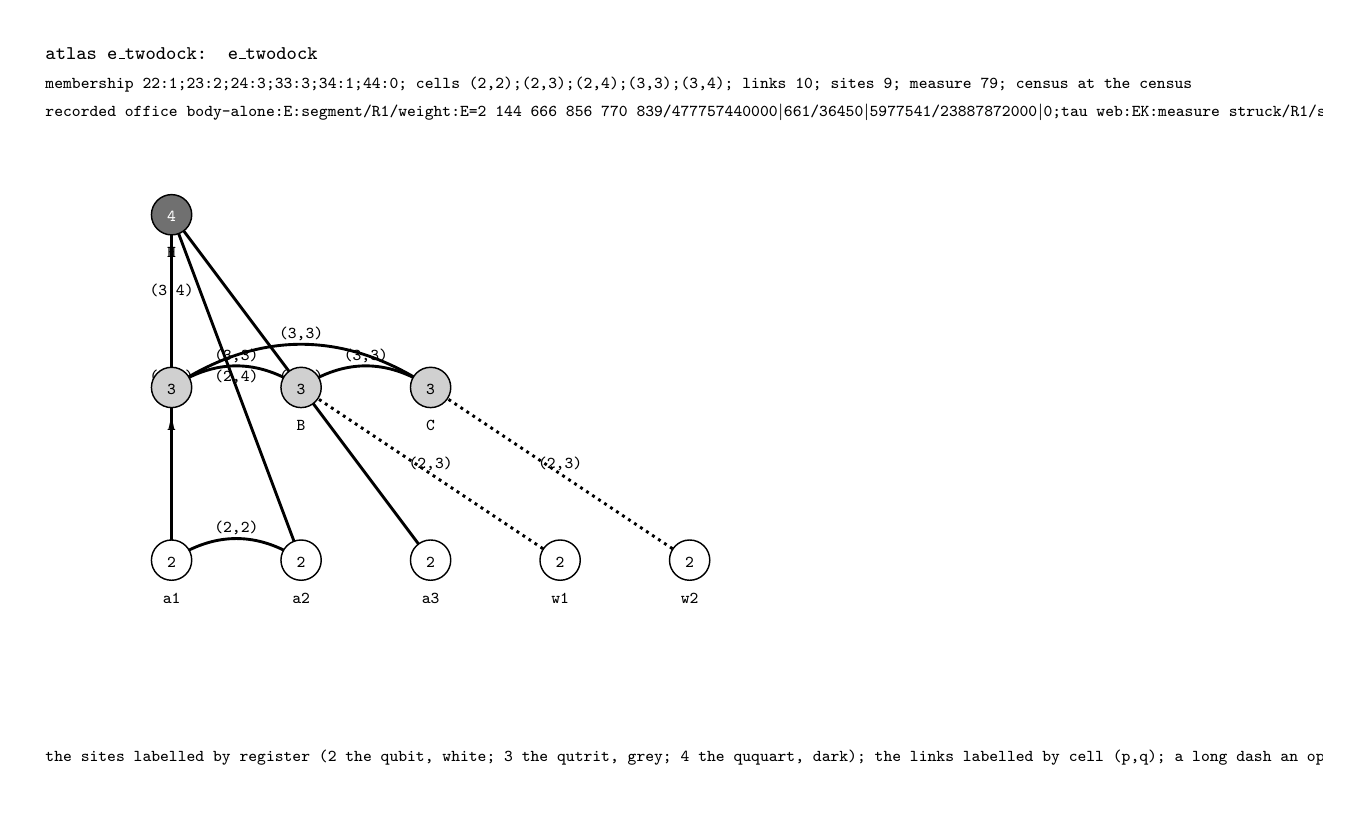
\begin{tikzpicture}[x=0.52pt,y=-0.52pt,baseline]
\clip (0,0) rectangle (900,540);
\fill[white] (0,0) rectangle (900,540);
\node[anchor=base west,inner sep=0pt,text=black,font=\fontsize{6.76}{8.112}\selectfont\ttfamily] at (12,22) {atlas e\_twodock: e\_twodock};
\node[anchor=base west,inner sep=0pt,text=black,font=\fontsize{6.24}{7.488}\selectfont\ttfamily] at (12,42) {membership 22:1;23:2;24:3;33:3;34:1;44:0; cells (2,2);(2,3);(2,4);(3,3);(3,4); links 10; sites 9; measure 79; census at the census};
\node[anchor=base west,inner sep=0pt,text=black,font=\fontsize{5.72}{6.864}\selectfont\ttfamily] at (12,62) {recorded office body-alone:E:segment/R1/weight:E=2 144 666 856 770 839/477757440000\textbar{}661/36450\textbar{}5977541/23887872000\textbar{}0;tau web:EK:measure struck/R1/slot/weight:EK=2 144 666 856 770 839/53084160000\textbar{}661/4050\textbar{}5977541/2654208000\textbar{}0; standing census:instrument;body-alone:theorem;hadron:open result;offices:theorem;nucleon:theorem;light-neutral office:theorem;formula:open result;tau web:theorem;roster:roster word; board electron};
\draw[draw=black,line width=1.04pt] (100,250) .. controls (130,230) and (160,230) .. (190,250);
\node[anchor=base,inner sep=0pt,text=black,font=\fontsize{5.72}{6.864}\selectfont\ttfamily] at (145,231) {(3,3)};
\draw[draw=black,line width=1.04pt] (100,250) .. controls (160,210) and (220,210) .. (280,250);
\node[anchor=base,inner sep=0pt,text=black,font=\fontsize{5.72}{6.864}\selectfont\ttfamily] at (190,216) {(3,3)};
\draw[draw=black,line width=1.04pt] (100,250) -- (100,130);
\node[anchor=base,inner sep=0pt,text=black,font=\fontsize{5.72}{6.864}\selectfont\ttfamily] at (100,186) {(3,4)};
\draw[draw=black,line width=1.04pt] (190,250) .. controls (220,230) and (250,230) .. (280,250);
\node[anchor=base,inner sep=0pt,text=black,font=\fontsize{5.72}{6.864}\selectfont\ttfamily] at (235,231) {(3,3)};
\draw[draw=black,line width=1.04pt,dash pattern=on 1.04pt off 1.56pt] (190,250) -- (370,370);
\node[anchor=base,inner sep=0pt,text=black,font=\fontsize{5.72}{6.864}\selectfont\ttfamily] at (280,306) {(2,3)};
\draw[draw=black,line width=1.04pt,dash pattern=on 1.04pt off 1.56pt] (280,250) -- (460,370);
\node[anchor=base,inner sep=0pt,text=black,font=\fontsize{5.72}{6.864}\selectfont\ttfamily] at (370,306) {(2,3)};
\draw[draw=black,line width=1.04pt] (100,130) -- (100,370);
\node[anchor=base,inner sep=0pt,text=black,font=\fontsize{5.72}{6.864}\selectfont\ttfamily] at (100,246) {(2,4)};
\draw[draw=black,line width=1.04pt] (100,130) -- (190,370);
\node[anchor=base,inner sep=0pt,text=black,font=\fontsize{5.72}{6.864}\selectfont\ttfamily] at (145,246) {(2,4)};
\draw[draw=black,line width=1.04pt] (100,130) -- (280,370);
\node[anchor=base,inner sep=0pt,text=black,font=\fontsize{5.72}{6.864}\selectfont\ttfamily] at (190,246) {(2,4)};
\draw[draw=black,line width=1.04pt] (100,370) .. controls (130,350) and (160,350) .. (190,370);
\node[anchor=base,inner sep=0pt,text=black,font=\fontsize{5.72}{6.864}\selectfont\ttfamily] at (145,351) {(2,2)};
\filldraw[fill={rgb,255:red,208;green,208;blue,208},draw=black,line width=0.52pt] (100,250) circle (14);
\node[anchor=base,inner sep=0pt,text=black,font=\fontsize{6.24}{7.488}\selectfont\ttfamily] at (100,255) {3};
\node[anchor=base,inner sep=0pt,text=black,font=\fontsize{5.72}{6.864}\selectfont\ttfamily] at (100,280) {A};
\filldraw[fill={rgb,255:red,208;green,208;blue,208},draw=black,line width=0.52pt] (190,250) circle (14);
\node[anchor=base,inner sep=0pt,text=black,font=\fontsize{6.24}{7.488}\selectfont\ttfamily] at (190,255) {3};
\node[anchor=base,inner sep=0pt,text=black,font=\fontsize{5.72}{6.864}\selectfont\ttfamily] at (190,280) {B};
\filldraw[fill={rgb,255:red,208;green,208;blue,208},draw=black,line width=0.52pt] (280,250) circle (14);
\node[anchor=base,inner sep=0pt,text=black,font=\fontsize{6.24}{7.488}\selectfont\ttfamily] at (280,255) {3};
\node[anchor=base,inner sep=0pt,text=black,font=\fontsize{5.72}{6.864}\selectfont\ttfamily] at (280,280) {C};
\filldraw[fill={rgb,255:red,112;green,112;blue,112},draw=black,line width=0.52pt] (100,130) circle (14);
\node[anchor=base,inner sep=0pt,text=white,font=\fontsize{6.24}{7.488}\selectfont\ttfamily] at (100,135) {4};
\node[anchor=base,inner sep=0pt,text=black,font=\fontsize{5.72}{6.864}\selectfont\ttfamily] at (100,160) {H};
\filldraw[fill=white,draw=black,line width=0.52pt] (100,370) circle (14);
\node[anchor=base,inner sep=0pt,text=black,font=\fontsize{6.24}{7.488}\selectfont\ttfamily] at (100,375) {2};
\node[anchor=base,inner sep=0pt,text=black,font=\fontsize{5.72}{6.864}\selectfont\ttfamily] at (100,400) {a1};
\filldraw[fill=white,draw=black,line width=0.52pt] (190,370) circle (14);
\node[anchor=base,inner sep=0pt,text=black,font=\fontsize{6.24}{7.488}\selectfont\ttfamily] at (190,375) {2};
\node[anchor=base,inner sep=0pt,text=black,font=\fontsize{5.72}{6.864}\selectfont\ttfamily] at (190,400) {a2};
\filldraw[fill=white,draw=black,line width=0.52pt] (280,370) circle (14);
\node[anchor=base,inner sep=0pt,text=black,font=\fontsize{6.24}{7.488}\selectfont\ttfamily] at (280,375) {2};
\node[anchor=base,inner sep=0pt,text=black,font=\fontsize{5.72}{6.864}\selectfont\ttfamily] at (280,400) {a3};
\filldraw[fill=white,draw=black,line width=0.52pt] (370,370) circle (14);
\node[anchor=base,inner sep=0pt,text=black,font=\fontsize{6.24}{7.488}\selectfont\ttfamily] at (370,375) {2};
\node[anchor=base,inner sep=0pt,text=black,font=\fontsize{5.72}{6.864}\selectfont\ttfamily] at (370,400) {w1};
\filldraw[fill=white,draw=black,line width=0.52pt] (460,370) circle (14);
\node[anchor=base,inner sep=0pt,text=black,font=\fontsize{6.24}{7.488}\selectfont\ttfamily] at (460,375) {2};
\node[anchor=base,inner sep=0pt,text=black,font=\fontsize{5.72}{6.864}\selectfont\ttfamily] at (460,400) {w2};
\node[anchor=base west,inner sep=0pt,text=black,font=\fontsize{5.72}{6.864}\selectfont\ttfamily] at (12,510) {the sites labelled by register (2 the qubit, white; 3 the qutrit, grey; 4 the ququart, dark); the links labelled by cell (p,q); a long dash an open dark link of the neutron row; a short dash a docked link at the rule R1};
\end{tikzpicture}
\caption{\texttt{e\_twodock} (the electron), beside, recorded body, hadron row body, roster body, roster web: 9 sites, 10 links, the measure 79; the links at the cells (2,2), (2,3), (2,4), (3,3), (3,4); the membership 22:1; 23:2; 24:3; 33:3; 34:1; 44:0; 2 docked links at the rule R1 (B-w1; C-w2); at the census of the six cells. Drawn at the anatomy atlas as its web, the sites labeled by register and the links by cell, from the the body-alone office rule.}\label{fig:VIII-2-D537322-e-twodock-2d8ced}
\begin{center}\footnotesize\begin{adjustbox}{max width=\linewidth}\begin{tabular}{p{0.26\textwidth}p{0.68\textwidth}}\toprule
recorded office (the slot-count row) & the read o-e of the formula row: the first power 67; the office \texttt{2 144 666 856 770 839/477757440000\textbar{}661/36450\textbar{}5977541/23887872000\textbar{}0}; against the formula with the slot count equal; the slot total 0; dark links 8; hubs H; dressing 1 \\
mass register (the mass-register row) & the read BE: the class touching the ququart; the first power 201; the office \texttt{2 144 666 856 770 839/53084160000\textbar{}661/4050\textbar{}5977541/2654208000\textbar{}0}; nonzero; met yes; hubs H; in-legs h-a; dressing 3; ports H-a3; B-w1; C-w2 \\
lepton-form office (the lepton row) & the read l-ek: the first power 67; the office \texttt{2 144 666 856 770 839/477757440000\textbar{}661/36450\textbar{}5977541/23887872000\textbar{}0}; against the cell equal; dark links 8 \\
\bottomrule\end{tabular}\end{adjustbox}\end{center}
\end{figure}
\begin{figure}[H]\centering
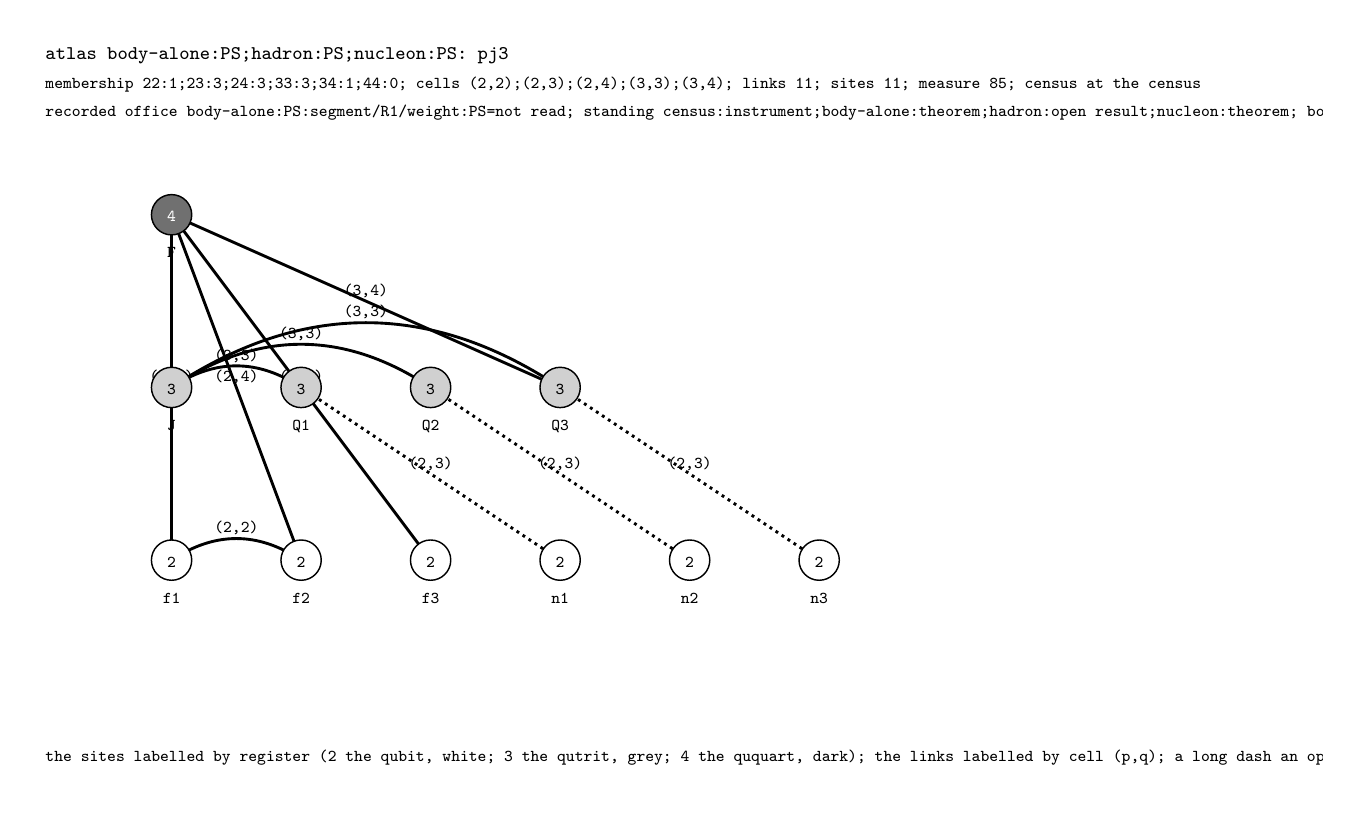
\begin{tikzpicture}[x=0.52pt,y=-0.52pt,baseline]
\clip (0,0) rectangle (900,540);
\fill[white] (0,0) rectangle (900,540);
\node[anchor=base west,inner sep=0pt,text=black,font=\fontsize{6.76}{8.112}\selectfont\ttfamily] at (12,22) {atlas body-alone:PS;hadron:PS;nucleon:PS: pj3};
\node[anchor=base west,inner sep=0pt,text=black,font=\fontsize{6.24}{7.488}\selectfont\ttfamily] at (12,42) {membership 22:1;23:3;24:3;33:3;34:1;44:0; cells (2,2);(2,3);(2,4);(3,3);(3,4); links 11; sites 11; measure 85; census at the census};
\node[anchor=base west,inner sep=0pt,text=black,font=\fontsize{5.72}{6.864}\selectfont\ttfamily] at (12,62) {recorded office body-alone:PS:segment/R1/weight:PS=not read; standing census:instrument;body-alone:theorem;hadron:open result;nucleon:theorem; board none};
\draw[draw=black,line width=1.04pt] (100,130) -- (370,250);
\node[anchor=base,inner sep=0pt,text=black,font=\fontsize{5.72}{6.864}\selectfont\ttfamily] at (235,186) {(3,4)};
\draw[draw=black,line width=1.04pt] (100,130) -- (100,370);
\node[anchor=base,inner sep=0pt,text=black,font=\fontsize{5.72}{6.864}\selectfont\ttfamily] at (100,246) {(2,4)};
\draw[draw=black,line width=1.04pt] (100,130) -- (190,370);
\node[anchor=base,inner sep=0pt,text=black,font=\fontsize{5.72}{6.864}\selectfont\ttfamily] at (145,246) {(2,4)};
\draw[draw=black,line width=1.04pt] (100,130) -- (280,370);
\node[anchor=base,inner sep=0pt,text=black,font=\fontsize{5.72}{6.864}\selectfont\ttfamily] at (190,246) {(2,4)};
\draw[draw=black,line width=1.04pt] (100,250) .. controls (130,230) and (160,230) .. (190,250);
\node[anchor=base,inner sep=0pt,text=black,font=\fontsize{5.72}{6.864}\selectfont\ttfamily] at (145,231) {(3,3)};
\draw[draw=black,line width=1.04pt] (100,250) .. controls (160,210) and (220,210) .. (280,250);
\node[anchor=base,inner sep=0pt,text=black,font=\fontsize{5.72}{6.864}\selectfont\ttfamily] at (190,216) {(3,3)};
\draw[draw=black,line width=1.04pt] (100,250) .. controls (190,190) and (280,190) .. (370,250);
\node[anchor=base,inner sep=0pt,text=black,font=\fontsize{5.72}{6.864}\selectfont\ttfamily] at (235,201) {(3,3)};
\draw[draw=black,line width=1.04pt,dash pattern=on 1.04pt off 1.56pt] (190,250) -- (370,370);
\node[anchor=base,inner sep=0pt,text=black,font=\fontsize{5.72}{6.864}\selectfont\ttfamily] at (280,306) {(2,3)};
\draw[draw=black,line width=1.04pt,dash pattern=on 1.04pt off 1.56pt] (280,250) -- (460,370);
\node[anchor=base,inner sep=0pt,text=black,font=\fontsize{5.72}{6.864}\selectfont\ttfamily] at (370,306) {(2,3)};
\draw[draw=black,line width=1.04pt,dash pattern=on 1.04pt off 1.56pt] (370,250) -- (550,370);
\node[anchor=base,inner sep=0pt,text=black,font=\fontsize{5.72}{6.864}\selectfont\ttfamily] at (460,306) {(2,3)};
\draw[draw=black,line width=1.04pt] (100,370) .. controls (130,350) and (160,350) .. (190,370);
\node[anchor=base,inner sep=0pt,text=black,font=\fontsize{5.72}{6.864}\selectfont\ttfamily] at (145,351) {(2,2)};
\filldraw[fill={rgb,255:red,112;green,112;blue,112},draw=black,line width=0.52pt] (100,130) circle (14);
\node[anchor=base,inner sep=0pt,text=white,font=\fontsize{6.24}{7.488}\selectfont\ttfamily] at (100,135) {4};
\node[anchor=base,inner sep=0pt,text=black,font=\fontsize{5.72}{6.864}\selectfont\ttfamily] at (100,160) {F};
\filldraw[fill={rgb,255:red,208;green,208;blue,208},draw=black,line width=0.52pt] (100,250) circle (14);
\node[anchor=base,inner sep=0pt,text=black,font=\fontsize{6.24}{7.488}\selectfont\ttfamily] at (100,255) {3};
\node[anchor=base,inner sep=0pt,text=black,font=\fontsize{5.72}{6.864}\selectfont\ttfamily] at (100,280) {J};
\filldraw[fill={rgb,255:red,208;green,208;blue,208},draw=black,line width=0.52pt] (190,250) circle (14);
\node[anchor=base,inner sep=0pt,text=black,font=\fontsize{6.24}{7.488}\selectfont\ttfamily] at (190,255) {3};
\node[anchor=base,inner sep=0pt,text=black,font=\fontsize{5.72}{6.864}\selectfont\ttfamily] at (190,280) {Q1};
\filldraw[fill={rgb,255:red,208;green,208;blue,208},draw=black,line width=0.52pt] (280,250) circle (14);
\node[anchor=base,inner sep=0pt,text=black,font=\fontsize{6.24}{7.488}\selectfont\ttfamily] at (280,255) {3};
\node[anchor=base,inner sep=0pt,text=black,font=\fontsize{5.72}{6.864}\selectfont\ttfamily] at (280,280) {Q2};
\filldraw[fill={rgb,255:red,208;green,208;blue,208},draw=black,line width=0.52pt] (370,250) circle (14);
\node[anchor=base,inner sep=0pt,text=black,font=\fontsize{6.24}{7.488}\selectfont\ttfamily] at (370,255) {3};
\node[anchor=base,inner sep=0pt,text=black,font=\fontsize{5.72}{6.864}\selectfont\ttfamily] at (370,280) {Q3};
\filldraw[fill=white,draw=black,line width=0.52pt] (100,370) circle (14);
\node[anchor=base,inner sep=0pt,text=black,font=\fontsize{6.24}{7.488}\selectfont\ttfamily] at (100,375) {2};
\node[anchor=base,inner sep=0pt,text=black,font=\fontsize{5.72}{6.864}\selectfont\ttfamily] at (100,400) {f1};
\filldraw[fill=white,draw=black,line width=0.52pt] (190,370) circle (14);
\node[anchor=base,inner sep=0pt,text=black,font=\fontsize{6.24}{7.488}\selectfont\ttfamily] at (190,375) {2};
\node[anchor=base,inner sep=0pt,text=black,font=\fontsize{5.72}{6.864}\selectfont\ttfamily] at (190,400) {f2};
\filldraw[fill=white,draw=black,line width=0.52pt] (280,370) circle (14);
\node[anchor=base,inner sep=0pt,text=black,font=\fontsize{6.24}{7.488}\selectfont\ttfamily] at (280,375) {2};
\node[anchor=base,inner sep=0pt,text=black,font=\fontsize{5.72}{6.864}\selectfont\ttfamily] at (280,400) {f3};
\filldraw[fill=white,draw=black,line width=0.52pt] (370,370) circle (14);
\node[anchor=base,inner sep=0pt,text=black,font=\fontsize{6.24}{7.488}\selectfont\ttfamily] at (370,375) {2};
\node[anchor=base,inner sep=0pt,text=black,font=\fontsize{5.72}{6.864}\selectfont\ttfamily] at (370,400) {n1};
\filldraw[fill=white,draw=black,line width=0.52pt] (460,370) circle (14);
\node[anchor=base,inner sep=0pt,text=black,font=\fontsize{6.24}{7.488}\selectfont\ttfamily] at (460,375) {2};
\node[anchor=base,inner sep=0pt,text=black,font=\fontsize{5.72}{6.864}\selectfont\ttfamily] at (460,400) {n2};
\filldraw[fill=white,draw=black,line width=0.52pt] (550,370) circle (14);
\node[anchor=base,inner sep=0pt,text=black,font=\fontsize{6.24}{7.488}\selectfont\ttfamily] at (550,375) {2};
\node[anchor=base,inner sep=0pt,text=black,font=\fontsize{5.72}{6.864}\selectfont\ttfamily] at (550,400) {n3};
\node[anchor=base west,inner sep=0pt,text=black,font=\fontsize{5.72}{6.864}\selectfont\ttfamily] at (12,510) {the sites labelled by register (2 the qubit, white; 3 the qutrit, grey; 4 the ququart, dark); the links labelled by cell (p,q); a long dash an open dark link of the neutron row; a short dash a docked link at the rule R1};
\end{tikzpicture}
\caption{\texttt{pj3}, hadron row body, junction star, star: 11 sites, 11 links, the measure 85; the links at the cells (2,2), (2,3), (2,4), (3,3), (3,4); the membership 22:1; 23:3; 24:3; 33:3; 34:1; 44:0; 3 docked links at the rule R1 (Q1-n1; Q2-n2; Q3-n3); at the census of the six cells. Drawn at the anatomy atlas as its web, the sites labeled by register and the links by cell, from the the body-alone office rule.}\label{fig:VIII-2-D537322-pj3-3a81f7}
\begin{center}\footnotesize\begin{adjustbox}{max width=\linewidth}\begin{tabular}{p{0.26\textwidth}p{0.68\textwidth}}\toprule
recorded office (the slot-count row) & the read d-ps of the hadron offices row: the first power 85; the office \texttt{7225\textbar{}0\textbar{}0\textbar{}0}; against the formula with the slot count parts; the slot total 0; dark links 8; hubs F; dressing 3 \\
mass register (the mass-register row) & the read bps: the class touching the ququart; the first power 201; the office \texttt{2 144 666 856 770 839/53084160000\textbar{}661/4050\textbar{}5977541/2654208000\textbar{}0}; nonzero; met yes; hubs F; in-legs Q3-F; dressing 3; ports Q1-n1; Q2-n2; Q3-n3; F-f3 \\
junction registers (the hadron row) & the read PS: junctions J; Q3; the share one third per leg; the registers at the share 85, struck 67, mono 255, the hub spelling 255; against the cells 85; 67; 255; 3, equal \\
\bottomrule\end{tabular}\end{adjustbox}\end{center}
\end{figure}
\begin{figure}[H]\centering
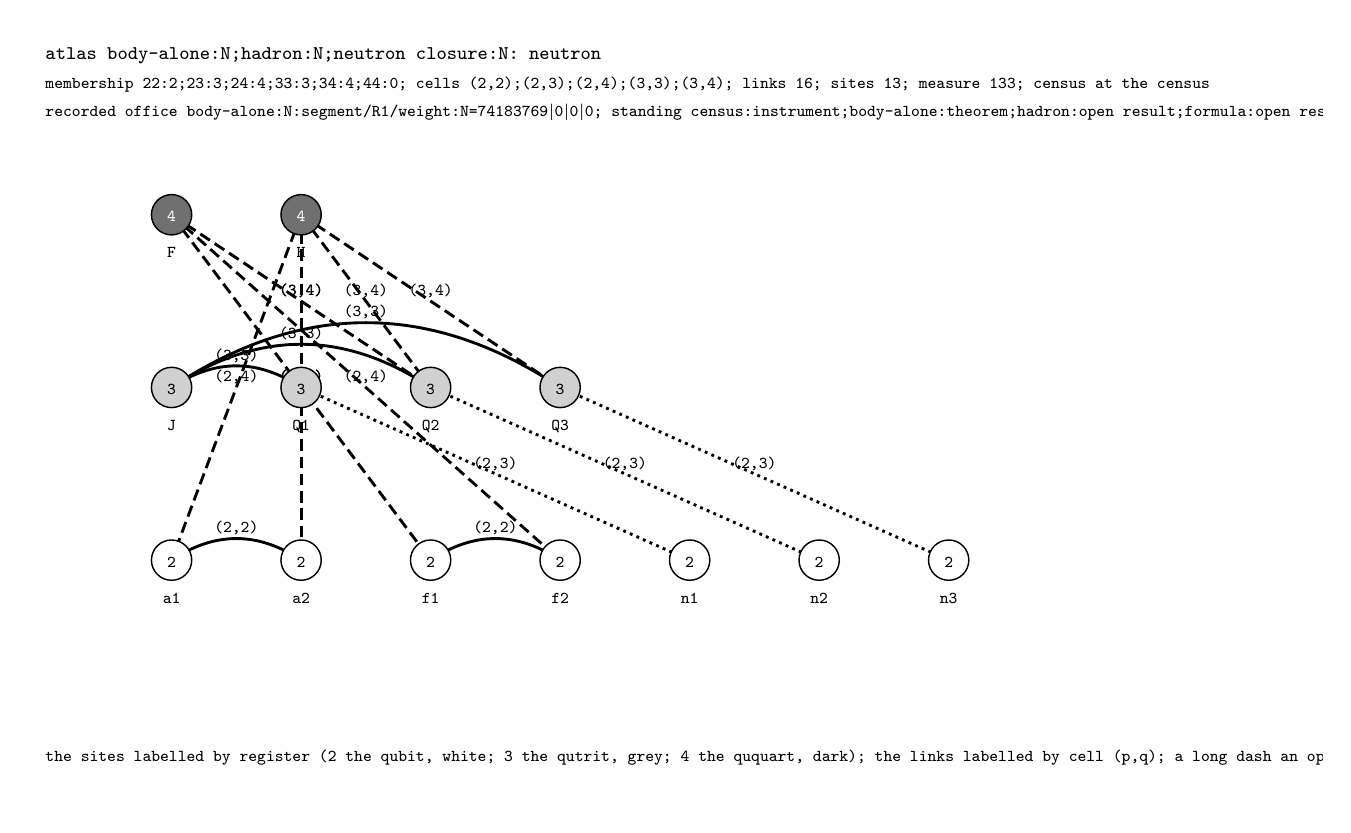
\begin{tikzpicture}[x=0.52pt,y=-0.52pt,baseline]
\clip (0,0) rectangle (900,540);
\fill[white] (0,0) rectangle (900,540);
\node[anchor=base west,inner sep=0pt,text=black,font=\fontsize{6.76}{8.112}\selectfont\ttfamily] at (12,22) {atlas body-alone:N;hadron:N;neutron closure:N: neutron};
\node[anchor=base west,inner sep=0pt,text=black,font=\fontsize{6.24}{7.488}\selectfont\ttfamily] at (12,42) {membership 22:2;23:3;24:4;33:3;34:4;44:0; cells (2,2);(2,3);(2,4);(3,3);(3,4); links 16; sites 13; measure 133; census at the census};
\node[anchor=base west,inner sep=0pt,text=black,font=\fontsize{5.72}{6.864}\selectfont\ttfamily] at (12,62) {recorded office body-alone:N:segment/R1/weight:N=74183769\textbar{}0\textbar{}0\textbar{}0; standing census:instrument;body-alone:theorem;hadron:open result;formula:open result;neutron closure:open result; board proton};
\draw[draw=black,line width=1.04pt,dash pattern=on 4.16pt off 2.08pt] (100,130) -- (280,250);
\node[anchor=base,inner sep=0pt,text=black,font=\fontsize{5.72}{6.864}\selectfont\ttfamily] at (190,186) {(3,4)};
\draw[draw=black,line width=1.04pt,dash pattern=on 4.16pt off 2.08pt] (100,130) -- (280,370);
\node[anchor=base,inner sep=0pt,text=black,font=\fontsize{5.72}{6.864}\selectfont\ttfamily] at (190,246) {(2,4)};
\draw[draw=black,line width=1.04pt,dash pattern=on 4.16pt off 2.08pt] (100,130) -- (370,370);
\node[anchor=base,inner sep=0pt,text=black,font=\fontsize{5.72}{6.864}\selectfont\ttfamily] at (235,246) {(2,4)};
\draw[draw=black,line width=1.04pt,dash pattern=on 4.16pt off 2.08pt] (190,130) -- (190,250);
\node[anchor=base,inner sep=0pt,text=black,font=\fontsize{5.72}{6.864}\selectfont\ttfamily] at (190,186) {(3,4)};
\draw[draw=black,line width=1.04pt,dash pattern=on 4.16pt off 2.08pt] (190,130) -- (280,250);
\node[anchor=base,inner sep=0pt,text=black,font=\fontsize{5.72}{6.864}\selectfont\ttfamily] at (235,186) {(3,4)};
\draw[draw=black,line width=1.04pt,dash pattern=on 4.16pt off 2.08pt] (190,130) -- (370,250);
\node[anchor=base,inner sep=0pt,text=black,font=\fontsize{5.72}{6.864}\selectfont\ttfamily] at (280,186) {(3,4)};
\draw[draw=black,line width=1.04pt,dash pattern=on 4.16pt off 2.08pt] (190,130) -- (100,370);
\node[anchor=base,inner sep=0pt,text=black,font=\fontsize{5.72}{6.864}\selectfont\ttfamily] at (145,246) {(2,4)};
\draw[draw=black,line width=1.04pt,dash pattern=on 4.16pt off 2.08pt] (190,130) -- (190,370);
\node[anchor=base,inner sep=0pt,text=black,font=\fontsize{5.72}{6.864}\selectfont\ttfamily] at (190,246) {(2,4)};
\draw[draw=black,line width=1.04pt] (100,250) .. controls (130,230) and (160,230) .. (190,250);
\node[anchor=base,inner sep=0pt,text=black,font=\fontsize{5.72}{6.864}\selectfont\ttfamily] at (145,231) {(3,3)};
\draw[draw=black,line width=1.04pt] (100,250) .. controls (160,210) and (220,210) .. (280,250);
\node[anchor=base,inner sep=0pt,text=black,font=\fontsize{5.72}{6.864}\selectfont\ttfamily] at (190,216) {(3,3)};
\draw[draw=black,line width=1.04pt] (100,250) .. controls (190,190) and (280,190) .. (370,250);
\node[anchor=base,inner sep=0pt,text=black,font=\fontsize{5.72}{6.864}\selectfont\ttfamily] at (235,201) {(3,3)};
\draw[draw=black,line width=1.04pt,dash pattern=on 1.04pt off 1.56pt] (190,250) -- (460,370);
\node[anchor=base,inner sep=0pt,text=black,font=\fontsize{5.72}{6.864}\selectfont\ttfamily] at (325,306) {(2,3)};
\draw[draw=black,line width=1.04pt,dash pattern=on 1.04pt off 1.56pt] (280,250) -- (550,370);
\node[anchor=base,inner sep=0pt,text=black,font=\fontsize{5.72}{6.864}\selectfont\ttfamily] at (415,306) {(2,3)};
\draw[draw=black,line width=1.04pt,dash pattern=on 1.04pt off 1.56pt] (370,250) -- (640,370);
\node[anchor=base,inner sep=0pt,text=black,font=\fontsize{5.72}{6.864}\selectfont\ttfamily] at (505,306) {(2,3)};
\draw[draw=black,line width=1.04pt] (100,370) .. controls (130,350) and (160,350) .. (190,370);
\node[anchor=base,inner sep=0pt,text=black,font=\fontsize{5.72}{6.864}\selectfont\ttfamily] at (145,351) {(2,2)};
\draw[draw=black,line width=1.04pt] (280,370) .. controls (310,350) and (340,350) .. (370,370);
\node[anchor=base,inner sep=0pt,text=black,font=\fontsize{5.72}{6.864}\selectfont\ttfamily] at (325,351) {(2,2)};
\filldraw[fill={rgb,255:red,112;green,112;blue,112},draw=black,line width=0.52pt] (100,130) circle (14);
\node[anchor=base,inner sep=0pt,text=white,font=\fontsize{6.24}{7.488}\selectfont\ttfamily] at (100,135) {4};
\node[anchor=base,inner sep=0pt,text=black,font=\fontsize{5.72}{6.864}\selectfont\ttfamily] at (100,160) {F};
\filldraw[fill={rgb,255:red,112;green,112;blue,112},draw=black,line width=0.52pt] (190,130) circle (14);
\node[anchor=base,inner sep=0pt,text=white,font=\fontsize{6.24}{7.488}\selectfont\ttfamily] at (190,135) {4};
\node[anchor=base,inner sep=0pt,text=black,font=\fontsize{5.72}{6.864}\selectfont\ttfamily] at (190,160) {H};
\filldraw[fill={rgb,255:red,208;green,208;blue,208},draw=black,line width=0.52pt] (100,250) circle (14);
\node[anchor=base,inner sep=0pt,text=black,font=\fontsize{6.24}{7.488}\selectfont\ttfamily] at (100,255) {3};
\node[anchor=base,inner sep=0pt,text=black,font=\fontsize{5.72}{6.864}\selectfont\ttfamily] at (100,280) {J};
\filldraw[fill={rgb,255:red,208;green,208;blue,208},draw=black,line width=0.52pt] (190,250) circle (14);
\node[anchor=base,inner sep=0pt,text=black,font=\fontsize{6.24}{7.488}\selectfont\ttfamily] at (190,255) {3};
\node[anchor=base,inner sep=0pt,text=black,font=\fontsize{5.72}{6.864}\selectfont\ttfamily] at (190,280) {Q1};
\filldraw[fill={rgb,255:red,208;green,208;blue,208},draw=black,line width=0.52pt] (280,250) circle (14);
\node[anchor=base,inner sep=0pt,text=black,font=\fontsize{6.24}{7.488}\selectfont\ttfamily] at (280,255) {3};
\node[anchor=base,inner sep=0pt,text=black,font=\fontsize{5.72}{6.864}\selectfont\ttfamily] at (280,280) {Q2};
\filldraw[fill={rgb,255:red,208;green,208;blue,208},draw=black,line width=0.52pt] (370,250) circle (14);
\node[anchor=base,inner sep=0pt,text=black,font=\fontsize{6.24}{7.488}\selectfont\ttfamily] at (370,255) {3};
\node[anchor=base,inner sep=0pt,text=black,font=\fontsize{5.72}{6.864}\selectfont\ttfamily] at (370,280) {Q3};
\filldraw[fill=white,draw=black,line width=0.52pt] (100,370) circle (14);
\node[anchor=base,inner sep=0pt,text=black,font=\fontsize{6.24}{7.488}\selectfont\ttfamily] at (100,375) {2};
\node[anchor=base,inner sep=0pt,text=black,font=\fontsize{5.72}{6.864}\selectfont\ttfamily] at (100,400) {a1};
\filldraw[fill=white,draw=black,line width=0.52pt] (190,370) circle (14);
\node[anchor=base,inner sep=0pt,text=black,font=\fontsize{6.24}{7.488}\selectfont\ttfamily] at (190,375) {2};
\node[anchor=base,inner sep=0pt,text=black,font=\fontsize{5.72}{6.864}\selectfont\ttfamily] at (190,400) {a2};
\filldraw[fill=white,draw=black,line width=0.52pt] (280,370) circle (14);
\node[anchor=base,inner sep=0pt,text=black,font=\fontsize{6.24}{7.488}\selectfont\ttfamily] at (280,375) {2};
\node[anchor=base,inner sep=0pt,text=black,font=\fontsize{5.72}{6.864}\selectfont\ttfamily] at (280,400) {f1};
\filldraw[fill=white,draw=black,line width=0.52pt] (370,370) circle (14);
\node[anchor=base,inner sep=0pt,text=black,font=\fontsize{6.24}{7.488}\selectfont\ttfamily] at (370,375) {2};
\node[anchor=base,inner sep=0pt,text=black,font=\fontsize{5.72}{6.864}\selectfont\ttfamily] at (370,400) {f2};
\filldraw[fill=white,draw=black,line width=0.52pt] (460,370) circle (14);
\node[anchor=base,inner sep=0pt,text=black,font=\fontsize{6.24}{7.488}\selectfont\ttfamily] at (460,375) {2};
\node[anchor=base,inner sep=0pt,text=black,font=\fontsize{5.72}{6.864}\selectfont\ttfamily] at (460,400) {n1};
\filldraw[fill=white,draw=black,line width=0.52pt] (550,370) circle (14);
\node[anchor=base,inner sep=0pt,text=black,font=\fontsize{6.24}{7.488}\selectfont\ttfamily] at (550,375) {2};
\node[anchor=base,inner sep=0pt,text=black,font=\fontsize{5.72}{6.864}\selectfont\ttfamily] at (550,400) {n2};
\filldraw[fill=white,draw=black,line width=0.52pt] (640,370) circle (14);
\node[anchor=base,inner sep=0pt,text=black,font=\fontsize{6.24}{7.488}\selectfont\ttfamily] at (640,375) {2};
\node[anchor=base,inner sep=0pt,text=black,font=\fontsize{5.72}{6.864}\selectfont\ttfamily] at (640,400) {n3};
\node[anchor=base west,inner sep=0pt,text=black,font=\fontsize{5.72}{6.864}\selectfont\ttfamily] at (12,510) {the sites labelled by register (2 the qubit, white; 3 the qutrit, grey; 4 the ququart, dark); the links labelled by cell (p,q); a long dash an open dark link of the neutron row; a short dash a docked link at the rule R1};
\end{tikzpicture}
\caption{\texttt{neutron} (the proton), recorded body, hadron row body, neutron at its own typing: 13 sites, 16 links, the measure 133; the links at the cells (2,2), (2,3), (2,4), (3,3), (3,4); the membership 22:2; 23:3; 24:4; 33:3; 34:4; 44:0; 3 docked links at the rule R1 (Q1-n1; Q2-n2; Q3-n3); 8 open dark links of the neutron row; at the census of the six cells. Drawn at the anatomy atlas as its web, the sites labeled by register and the links by cell, from the the body-alone office rule.}\label{fig:VIII-2-D537322-neutron-9be5ea}
\begin{center}\footnotesize\begin{adjustbox}{max width=\linewidth}\begin{tabular}{p{0.26\textwidth}p{0.68\textwidth}}\toprule
recorded office (the slot-count row) & the read o-n of the formula row: the first power 8613; the office \texttt{74183769\textbar{}0\textbar{}0\textbar{}0}; against the formula with the slot count equal; the slot total 1; dark links 13; hubs H; F; dressing 27 \\
mass register (the mass-register row) & the read BN: the class touching the ququart; the first power 9315; the office \texttt{56 865 317 258 729 151/655360000\textbar{}5841/25\textbar{}320665041/163840000\textbar{}0}; nonzero; met yes; hubs F; H; in-legs H-Q1; H-Q2; H-Q3; Q2-F; dressing 81; ports Q1-n1; Q2-n2; Q3-n3 \\
junction registers (the hadron row) & the read N: junctions J; Q1; Q3; the share one third per leg; the registers at the share 133, struck 115, mono 1596, the hub spelling 3591; against the cells none; none; none; none, none \\
\bottomrule\end{tabular}\end{adjustbox}\end{center}
\end{figure}
\begin{figure}[H]\centering
\begin{adjustbox}{max width=\linewidth}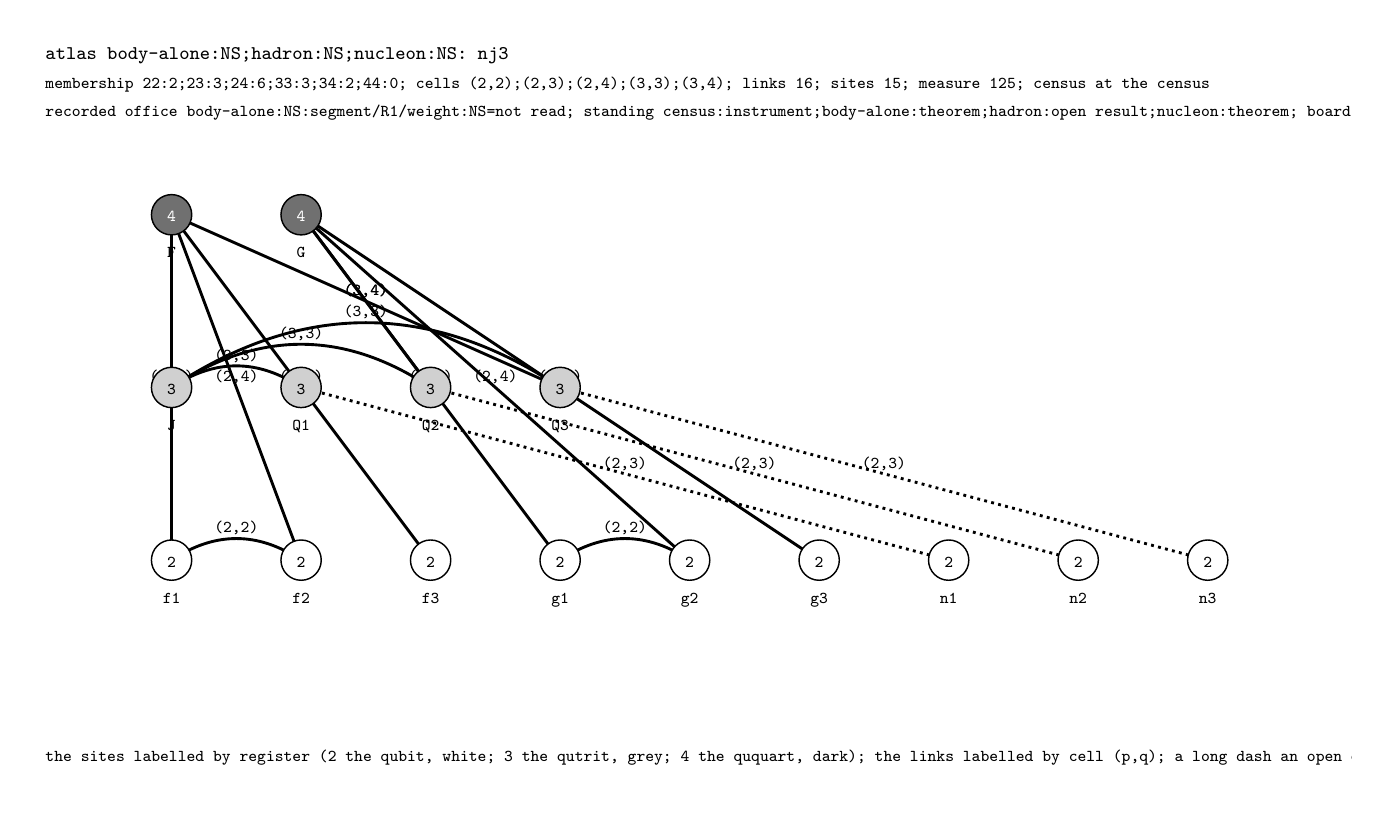
\begin{tikzpicture}[x=0.52pt,y=-0.52pt,baseline]
\clip (0,0) rectangle (920,540);
\fill[white] (0,0) rectangle (920,540);
\node[anchor=base west,inner sep=0pt,text=black,font=\fontsize{6.76}{8.112}\selectfont\ttfamily] at (12,22) {atlas body-alone:NS;hadron:NS;nucleon:NS: nj3};
\node[anchor=base west,inner sep=0pt,text=black,font=\fontsize{6.24}{7.488}\selectfont\ttfamily] at (12,42) {membership 22:2;23:3;24:6;33:3;34:2;44:0; cells (2,2);(2,3);(2,4);(3,3);(3,4); links 16; sites 15; measure 125; census at the census};
\node[anchor=base west,inner sep=0pt,text=black,font=\fontsize{5.72}{6.864}\selectfont\ttfamily] at (12,62) {recorded office body-alone:NS:segment/R1/weight:NS=not read; standing census:instrument;body-alone:theorem;hadron:open result;nucleon:theorem; board none};
\draw[draw=black,line width=1.04pt] (100,130) -- (370,250);
\node[anchor=base,inner sep=0pt,text=black,font=\fontsize{5.72}{6.864}\selectfont\ttfamily] at (235,186) {(3,4)};
\draw[draw=black,line width=1.04pt] (100,130) -- (100,370);
\node[anchor=base,inner sep=0pt,text=black,font=\fontsize{5.72}{6.864}\selectfont\ttfamily] at (100,246) {(2,4)};
\draw[draw=black,line width=1.04pt] (100,130) -- (190,370);
\node[anchor=base,inner sep=0pt,text=black,font=\fontsize{5.72}{6.864}\selectfont\ttfamily] at (145,246) {(2,4)};
\draw[draw=black,line width=1.04pt] (100,130) -- (280,370);
\node[anchor=base,inner sep=0pt,text=black,font=\fontsize{5.72}{6.864}\selectfont\ttfamily] at (190,246) {(2,4)};
\draw[draw=black,line width=1.04pt] (190,130) -- (280,250);
\node[anchor=base,inner sep=0pt,text=black,font=\fontsize{5.72}{6.864}\selectfont\ttfamily] at (235,186) {(3,4)};
\draw[draw=black,line width=1.04pt] (190,130) -- (370,370);
\node[anchor=base,inner sep=0pt,text=black,font=\fontsize{5.72}{6.864}\selectfont\ttfamily] at (280,246) {(2,4)};
\draw[draw=black,line width=1.04pt] (190,130) -- (460,370);
\node[anchor=base,inner sep=0pt,text=black,font=\fontsize{5.72}{6.864}\selectfont\ttfamily] at (325,246) {(2,4)};
\draw[draw=black,line width=1.04pt] (190,130) -- (550,370);
\node[anchor=base,inner sep=0pt,text=black,font=\fontsize{5.72}{6.864}\selectfont\ttfamily] at (370,246) {(2,4)};
\draw[draw=black,line width=1.04pt] (100,250) .. controls (130,230) and (160,230) .. (190,250);
\node[anchor=base,inner sep=0pt,text=black,font=\fontsize{5.72}{6.864}\selectfont\ttfamily] at (145,231) {(3,3)};
\draw[draw=black,line width=1.04pt] (100,250) .. controls (160,210) and (220,210) .. (280,250);
\node[anchor=base,inner sep=0pt,text=black,font=\fontsize{5.72}{6.864}\selectfont\ttfamily] at (190,216) {(3,3)};
\draw[draw=black,line width=1.04pt] (100,250) .. controls (190,190) and (280,190) .. (370,250);
\node[anchor=base,inner sep=0pt,text=black,font=\fontsize{5.72}{6.864}\selectfont\ttfamily] at (235,201) {(3,3)};
\draw[draw=black,line width=1.04pt,dash pattern=on 1.04pt off 1.56pt] (190,250) -- (640,370);
\node[anchor=base,inner sep=0pt,text=black,font=\fontsize{5.72}{6.864}\selectfont\ttfamily] at (415,306) {(2,3)};
\draw[draw=black,line width=1.04pt,dash pattern=on 1.04pt off 1.56pt] (280,250) -- (730,370);
\node[anchor=base,inner sep=0pt,text=black,font=\fontsize{5.72}{6.864}\selectfont\ttfamily] at (505,306) {(2,3)};
\draw[draw=black,line width=1.04pt,dash pattern=on 1.04pt off 1.56pt] (370,250) -- (820,370);
\node[anchor=base,inner sep=0pt,text=black,font=\fontsize{5.72}{6.864}\selectfont\ttfamily] at (595,306) {(2,3)};
\draw[draw=black,line width=1.04pt] (100,370) .. controls (130,350) and (160,350) .. (190,370);
\node[anchor=base,inner sep=0pt,text=black,font=\fontsize{5.72}{6.864}\selectfont\ttfamily] at (145,351) {(2,2)};
\draw[draw=black,line width=1.04pt] (370,370) .. controls (400,350) and (430,350) .. (460,370);
\node[anchor=base,inner sep=0pt,text=black,font=\fontsize{5.72}{6.864}\selectfont\ttfamily] at (415,351) {(2,2)};
\filldraw[fill={rgb,255:red,112;green,112;blue,112},draw=black,line width=0.52pt] (100,130) circle (14);
\node[anchor=base,inner sep=0pt,text=white,font=\fontsize{6.24}{7.488}\selectfont\ttfamily] at (100,135) {4};
\node[anchor=base,inner sep=0pt,text=black,font=\fontsize{5.72}{6.864}\selectfont\ttfamily] at (100,160) {F};
\filldraw[fill={rgb,255:red,112;green,112;blue,112},draw=black,line width=0.52pt] (190,130) circle (14);
\node[anchor=base,inner sep=0pt,text=white,font=\fontsize{6.24}{7.488}\selectfont\ttfamily] at (190,135) {4};
\node[anchor=base,inner sep=0pt,text=black,font=\fontsize{5.72}{6.864}\selectfont\ttfamily] at (190,160) {G};
\filldraw[fill={rgb,255:red,208;green,208;blue,208},draw=black,line width=0.52pt] (100,250) circle (14);
\node[anchor=base,inner sep=0pt,text=black,font=\fontsize{6.24}{7.488}\selectfont\ttfamily] at (100,255) {3};
\node[anchor=base,inner sep=0pt,text=black,font=\fontsize{5.72}{6.864}\selectfont\ttfamily] at (100,280) {J};
\filldraw[fill={rgb,255:red,208;green,208;blue,208},draw=black,line width=0.52pt] (190,250) circle (14);
\node[anchor=base,inner sep=0pt,text=black,font=\fontsize{6.24}{7.488}\selectfont\ttfamily] at (190,255) {3};
\node[anchor=base,inner sep=0pt,text=black,font=\fontsize{5.72}{6.864}\selectfont\ttfamily] at (190,280) {Q1};
\filldraw[fill={rgb,255:red,208;green,208;blue,208},draw=black,line width=0.52pt] (280,250) circle (14);
\node[anchor=base,inner sep=0pt,text=black,font=\fontsize{6.24}{7.488}\selectfont\ttfamily] at (280,255) {3};
\node[anchor=base,inner sep=0pt,text=black,font=\fontsize{5.72}{6.864}\selectfont\ttfamily] at (280,280) {Q2};
\filldraw[fill={rgb,255:red,208;green,208;blue,208},draw=black,line width=0.52pt] (370,250) circle (14);
\node[anchor=base,inner sep=0pt,text=black,font=\fontsize{6.24}{7.488}\selectfont\ttfamily] at (370,255) {3};
\node[anchor=base,inner sep=0pt,text=black,font=\fontsize{5.72}{6.864}\selectfont\ttfamily] at (370,280) {Q3};
\filldraw[fill=white,draw=black,line width=0.52pt] (100,370) circle (14);
\node[anchor=base,inner sep=0pt,text=black,font=\fontsize{6.24}{7.488}\selectfont\ttfamily] at (100,375) {2};
\node[anchor=base,inner sep=0pt,text=black,font=\fontsize{5.72}{6.864}\selectfont\ttfamily] at (100,400) {f1};
\filldraw[fill=white,draw=black,line width=0.52pt] (190,370) circle (14);
\node[anchor=base,inner sep=0pt,text=black,font=\fontsize{6.24}{7.488}\selectfont\ttfamily] at (190,375) {2};
\node[anchor=base,inner sep=0pt,text=black,font=\fontsize{5.72}{6.864}\selectfont\ttfamily] at (190,400) {f2};
\filldraw[fill=white,draw=black,line width=0.52pt] (280,370) circle (14);
\node[anchor=base,inner sep=0pt,text=black,font=\fontsize{6.24}{7.488}\selectfont\ttfamily] at (280,375) {2};
\node[anchor=base,inner sep=0pt,text=black,font=\fontsize{5.72}{6.864}\selectfont\ttfamily] at (280,400) {f3};
\filldraw[fill=white,draw=black,line width=0.52pt] (370,370) circle (14);
\node[anchor=base,inner sep=0pt,text=black,font=\fontsize{6.24}{7.488}\selectfont\ttfamily] at (370,375) {2};
\node[anchor=base,inner sep=0pt,text=black,font=\fontsize{5.72}{6.864}\selectfont\ttfamily] at (370,400) {g1};
\filldraw[fill=white,draw=black,line width=0.52pt] (460,370) circle (14);
\node[anchor=base,inner sep=0pt,text=black,font=\fontsize{6.24}{7.488}\selectfont\ttfamily] at (460,375) {2};
\node[anchor=base,inner sep=0pt,text=black,font=\fontsize{5.72}{6.864}\selectfont\ttfamily] at (460,400) {g2};
\filldraw[fill=white,draw=black,line width=0.52pt] (550,370) circle (14);
\node[anchor=base,inner sep=0pt,text=black,font=\fontsize{6.24}{7.488}\selectfont\ttfamily] at (550,375) {2};
\node[anchor=base,inner sep=0pt,text=black,font=\fontsize{5.72}{6.864}\selectfont\ttfamily] at (550,400) {g3};
\filldraw[fill=white,draw=black,line width=0.52pt] (640,370) circle (14);
\node[anchor=base,inner sep=0pt,text=black,font=\fontsize{6.24}{7.488}\selectfont\ttfamily] at (640,375) {2};
\node[anchor=base,inner sep=0pt,text=black,font=\fontsize{5.72}{6.864}\selectfont\ttfamily] at (640,400) {n1};
\filldraw[fill=white,draw=black,line width=0.52pt] (730,370) circle (14);
\node[anchor=base,inner sep=0pt,text=black,font=\fontsize{6.24}{7.488}\selectfont\ttfamily] at (730,375) {2};
\node[anchor=base,inner sep=0pt,text=black,font=\fontsize{5.72}{6.864}\selectfont\ttfamily] at (730,400) {n2};
\filldraw[fill=white,draw=black,line width=0.52pt] (820,370) circle (14);
\node[anchor=base,inner sep=0pt,text=black,font=\fontsize{6.24}{7.488}\selectfont\ttfamily] at (820,375) {2};
\node[anchor=base,inner sep=0pt,text=black,font=\fontsize{5.72}{6.864}\selectfont\ttfamily] at (820,400) {n3};
\node[anchor=base west,inner sep=0pt,text=black,font=\fontsize{5.72}{6.864}\selectfont\ttfamily] at (12,510) {the sites labelled by register (2 the qubit, white; 3 the qutrit, grey; 4 the ququart, dark); the links labelled by cell (p,q); a long dash an open dark link of the neutron row; a short dash a docked link at the rule R1};
\end{tikzpicture}\end{adjustbox}
\caption{\texttt{nj3}, hadron row body, junction star, star: 15 sites, 16 links, the measure 125; the links at the cells (2,2), (2,3), (2,4), (3,3), (3,4); the membership 22:2; 23:3; 24:6; 33:3; 34:2; 44:0; 3 docked links at the rule R1 (Q1-n1; Q2-n2; Q3-n3); at the census of the six cells. Drawn at the anatomy atlas as its web, the sites labeled by register and the links by cell, from the the body-alone office rule.}\label{fig:VIII-2-D537322-nj3-b62b70}
\begin{center}\footnotesize\begin{adjustbox}{max width=\linewidth}\begin{tabular}{p{0.26\textwidth}p{0.68\textwidth}}\toprule
recorded office (the slot-count row) & no read of this body at the slot-count row \\
mass register (the mass-register row) & the read bns: the class touching the ququart; the first power 963; the office \texttt{5 469 872 145 467 303/5898240000\textbar{}661/225\textbar{}6301957/294912000\textbar{}0}; nonzero; met yes; hubs F; G; in-legs Q3-F; Q2-G; dressing 9; ports Q1-n1; Q2-n2; Q3-n3; F-f3; G-g3 \\
junction registers (the hadron row) & the read NS: junctions J; Q2; Q3; the share one third per leg; the registers at the share 125, struck 107, mono 1125, the hub spelling 1125; against the cells 125; 107; 1125; 9, equal \\
\bottomrule\end{tabular}\end{adjustbox}\end{center}
\end{figure}
\begin{figure}[H]\centering
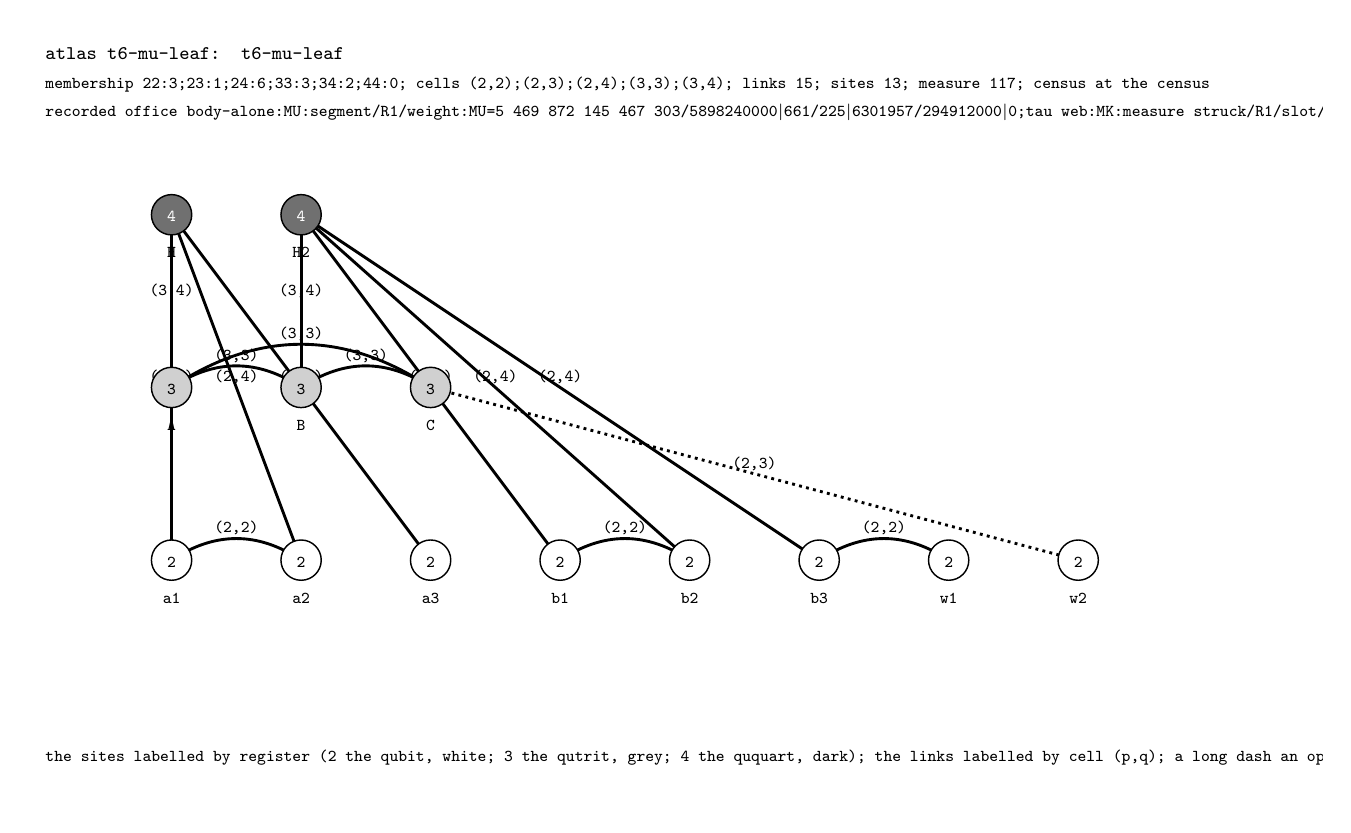
\begin{tikzpicture}[x=0.52pt,y=-0.52pt,baseline]
\clip (0,0) rectangle (900,540);
\fill[white] (0,0) rectangle (900,540);
\node[anchor=base west,inner sep=0pt,text=black,font=\fontsize{6.76}{8.112}\selectfont\ttfamily] at (12,22) {atlas t6-mu-leaf: t6-mu-leaf};
\node[anchor=base west,inner sep=0pt,text=black,font=\fontsize{6.24}{7.488}\selectfont\ttfamily] at (12,42) {membership 22:3;23:1;24:6;33:3;34:2;44:0; cells (2,2);(2,3);(2,4);(3,3);(3,4); links 15; sites 13; measure 117; census at the census};
\node[anchor=base west,inner sep=0pt,text=black,font=\fontsize{5.72}{6.864}\selectfont\ttfamily] at (12,62) {recorded office body-alone:MU:segment/R1/weight:MU=5 469 872 145 467 303/5898240000\textbar{}661/225\textbar{}6301957/294912000\textbar{}0;tau web:MK:measure struck/R1/slot/weight:MK=5 469 872 145 467 303/5898240000\textbar{}661/225\textbar{}6301957/294912000\textbar{}0; standing census:instrument;body-alone:theorem;formula:open result;tau web:theorem;roster:roster word; board muon};
\draw[draw=black,line width=1.04pt] (100,250) .. controls (130,230) and (160,230) .. (190,250);
\node[anchor=base,inner sep=0pt,text=black,font=\fontsize{5.72}{6.864}\selectfont\ttfamily] at (145,231) {(3,3)};
\draw[draw=black,line width=1.04pt] (100,250) .. controls (160,210) and (220,210) .. (280,250);
\node[anchor=base,inner sep=0pt,text=black,font=\fontsize{5.72}{6.864}\selectfont\ttfamily] at (190,216) {(3,3)};
\draw[draw=black,line width=1.04pt] (100,250) -- (100,130);
\node[anchor=base,inner sep=0pt,text=black,font=\fontsize{5.72}{6.864}\selectfont\ttfamily] at (100,186) {(3,4)};
\draw[draw=black,line width=1.04pt] (190,250) .. controls (220,230) and (250,230) .. (280,250);
\node[anchor=base,inner sep=0pt,text=black,font=\fontsize{5.72}{6.864}\selectfont\ttfamily] at (235,231) {(3,3)};
\draw[draw=black,line width=1.04pt] (190,250) -- (190,130);
\node[anchor=base,inner sep=0pt,text=black,font=\fontsize{5.72}{6.864}\selectfont\ttfamily] at (190,186) {(3,4)};
\draw[draw=black,line width=1.04pt,dash pattern=on 1.04pt off 1.56pt] (280,250) -- (730,370);
\node[anchor=base,inner sep=0pt,text=black,font=\fontsize{5.72}{6.864}\selectfont\ttfamily] at (505,306) {(2,3)};
\draw[draw=black,line width=1.04pt] (100,130) -- (100,370);
\node[anchor=base,inner sep=0pt,text=black,font=\fontsize{5.72}{6.864}\selectfont\ttfamily] at (100,246) {(2,4)};
\draw[draw=black,line width=1.04pt] (100,130) -- (190,370);
\node[anchor=base,inner sep=0pt,text=black,font=\fontsize{5.72}{6.864}\selectfont\ttfamily] at (145,246) {(2,4)};
\draw[draw=black,line width=1.04pt] (100,130) -- (280,370);
\node[anchor=base,inner sep=0pt,text=black,font=\fontsize{5.72}{6.864}\selectfont\ttfamily] at (190,246) {(2,4)};
\draw[draw=black,line width=1.04pt] (190,130) -- (370,370);
\node[anchor=base,inner sep=0pt,text=black,font=\fontsize{5.72}{6.864}\selectfont\ttfamily] at (280,246) {(2,4)};
\draw[draw=black,line width=1.04pt] (190,130) -- (460,370);
\node[anchor=base,inner sep=0pt,text=black,font=\fontsize{5.72}{6.864}\selectfont\ttfamily] at (325,246) {(2,4)};
\draw[draw=black,line width=1.04pt] (190,130) -- (550,370);
\node[anchor=base,inner sep=0pt,text=black,font=\fontsize{5.72}{6.864}\selectfont\ttfamily] at (370,246) {(2,4)};
\draw[draw=black,line width=1.04pt] (100,370) .. controls (130,350) and (160,350) .. (190,370);
\node[anchor=base,inner sep=0pt,text=black,font=\fontsize{5.72}{6.864}\selectfont\ttfamily] at (145,351) {(2,2)};
\draw[draw=black,line width=1.04pt] (370,370) .. controls (400,350) and (430,350) .. (460,370);
\node[anchor=base,inner sep=0pt,text=black,font=\fontsize{5.72}{6.864}\selectfont\ttfamily] at (415,351) {(2,2)};
\draw[draw=black,line width=1.04pt] (550,370) .. controls (580,350) and (610,350) .. (640,370);
\node[anchor=base,inner sep=0pt,text=black,font=\fontsize{5.72}{6.864}\selectfont\ttfamily] at (595,351) {(2,2)};
\filldraw[fill={rgb,255:red,208;green,208;blue,208},draw=black,line width=0.52pt] (100,250) circle (14);
\node[anchor=base,inner sep=0pt,text=black,font=\fontsize{6.24}{7.488}\selectfont\ttfamily] at (100,255) {3};
\node[anchor=base,inner sep=0pt,text=black,font=\fontsize{5.72}{6.864}\selectfont\ttfamily] at (100,280) {A};
\filldraw[fill={rgb,255:red,208;green,208;blue,208},draw=black,line width=0.52pt] (190,250) circle (14);
\node[anchor=base,inner sep=0pt,text=black,font=\fontsize{6.24}{7.488}\selectfont\ttfamily] at (190,255) {3};
\node[anchor=base,inner sep=0pt,text=black,font=\fontsize{5.72}{6.864}\selectfont\ttfamily] at (190,280) {B};
\filldraw[fill={rgb,255:red,208;green,208;blue,208},draw=black,line width=0.52pt] (280,250) circle (14);
\node[anchor=base,inner sep=0pt,text=black,font=\fontsize{6.24}{7.488}\selectfont\ttfamily] at (280,255) {3};
\node[anchor=base,inner sep=0pt,text=black,font=\fontsize{5.72}{6.864}\selectfont\ttfamily] at (280,280) {C};
\filldraw[fill={rgb,255:red,112;green,112;blue,112},draw=black,line width=0.52pt] (100,130) circle (14);
\node[anchor=base,inner sep=0pt,text=white,font=\fontsize{6.24}{7.488}\selectfont\ttfamily] at (100,135) {4};
\node[anchor=base,inner sep=0pt,text=black,font=\fontsize{5.72}{6.864}\selectfont\ttfamily] at (100,160) {H};
\filldraw[fill={rgb,255:red,112;green,112;blue,112},draw=black,line width=0.52pt] (190,130) circle (14);
\node[anchor=base,inner sep=0pt,text=white,font=\fontsize{6.24}{7.488}\selectfont\ttfamily] at (190,135) {4};
\node[anchor=base,inner sep=0pt,text=black,font=\fontsize{5.72}{6.864}\selectfont\ttfamily] at (190,160) {H2};
\filldraw[fill=white,draw=black,line width=0.52pt] (100,370) circle (14);
\node[anchor=base,inner sep=0pt,text=black,font=\fontsize{6.24}{7.488}\selectfont\ttfamily] at (100,375) {2};
\node[anchor=base,inner sep=0pt,text=black,font=\fontsize{5.72}{6.864}\selectfont\ttfamily] at (100,400) {a1};
\filldraw[fill=white,draw=black,line width=0.52pt] (190,370) circle (14);
\node[anchor=base,inner sep=0pt,text=black,font=\fontsize{6.24}{7.488}\selectfont\ttfamily] at (190,375) {2};
\node[anchor=base,inner sep=0pt,text=black,font=\fontsize{5.72}{6.864}\selectfont\ttfamily] at (190,400) {a2};
\filldraw[fill=white,draw=black,line width=0.52pt] (280,370) circle (14);
\node[anchor=base,inner sep=0pt,text=black,font=\fontsize{6.24}{7.488}\selectfont\ttfamily] at (280,375) {2};
\node[anchor=base,inner sep=0pt,text=black,font=\fontsize{5.72}{6.864}\selectfont\ttfamily] at (280,400) {a3};
\filldraw[fill=white,draw=black,line width=0.52pt] (370,370) circle (14);
\node[anchor=base,inner sep=0pt,text=black,font=\fontsize{6.24}{7.488}\selectfont\ttfamily] at (370,375) {2};
\node[anchor=base,inner sep=0pt,text=black,font=\fontsize{5.72}{6.864}\selectfont\ttfamily] at (370,400) {b1};
\filldraw[fill=white,draw=black,line width=0.52pt] (460,370) circle (14);
\node[anchor=base,inner sep=0pt,text=black,font=\fontsize{6.24}{7.488}\selectfont\ttfamily] at (460,375) {2};
\node[anchor=base,inner sep=0pt,text=black,font=\fontsize{5.72}{6.864}\selectfont\ttfamily] at (460,400) {b2};
\filldraw[fill=white,draw=black,line width=0.52pt] (550,370) circle (14);
\node[anchor=base,inner sep=0pt,text=black,font=\fontsize{6.24}{7.488}\selectfont\ttfamily] at (550,375) {2};
\node[anchor=base,inner sep=0pt,text=black,font=\fontsize{5.72}{6.864}\selectfont\ttfamily] at (550,400) {b3};
\filldraw[fill=white,draw=black,line width=0.52pt] (640,370) circle (14);
\node[anchor=base,inner sep=0pt,text=black,font=\fontsize{6.24}{7.488}\selectfont\ttfamily] at (640,375) {2};
\node[anchor=base,inner sep=0pt,text=black,font=\fontsize{5.72}{6.864}\selectfont\ttfamily] at (640,400) {w1};
\filldraw[fill=white,draw=black,line width=0.52pt] (730,370) circle (14);
\node[anchor=base,inner sep=0pt,text=black,font=\fontsize{6.24}{7.488}\selectfont\ttfamily] at (730,375) {2};
\node[anchor=base,inner sep=0pt,text=black,font=\fontsize{5.72}{6.864}\selectfont\ttfamily] at (730,400) {w2};
\node[anchor=base west,inner sep=0pt,text=black,font=\fontsize{5.72}{6.864}\selectfont\ttfamily] at (12,510) {the sites labelled by register (2 the qubit, white; 3 the qutrit, grey; 4 the ququart, dark); the links labelled by cell (p,q); a long dash an open dark link of the neutron row; a short dash a docked link at the rule R1};
\end{tikzpicture}
\caption{\texttt{t6-mu-leaf} (the muon), recorded body, roster web: 13 sites, 15 links, the measure 117; the links at the cells (2,2), (2,3), (2,4), (3,3), (3,4); the membership 22:3; 23:1; 24:6; 33:3; 34:2; 44:0; 1 docked links at the rule R1 (w2-C); at the census of the six cells. Drawn at the anatomy atlas as its web, the sites labeled by register and the links by cell, from the the body-alone office rule.}\label{fig:VIII-2-D537322-t6-mu-leaf-7c6b2e}
\begin{center}\footnotesize\begin{adjustbox}{max width=\linewidth}\begin{tabular}{p{0.26\textwidth}p{0.68\textwidth}}\toprule
recorded office (the slot-count row) & the read o-mu of the formula row: the first power 963; the office \texttt{5 469 872 145 467 303/5898240000\textbar{}661/225\textbar{}6301957/294912000\textbar{}0}; against the formula with the slot count equal; the slot total 0; dark links 14; hubs H; H2; dressing 9 \\
mass register (the mass-register row) & the read bmu: the class touching the ququart; the first power 963; the office \texttt{5 469 872 145 467 303/5898240000\textbar{}661/225\textbar{}6301957/294912000\textbar{}0}; nonzero; met yes; hubs H; H2; in-legs h-a; H2-B; dressing 9; ports H-a3; w2-C; w1-b3 \\
lepton-form office (the lepton row) & the read l-mk: the first power 963; the office \texttt{5 469 872 145 467 303/5898240000\textbar{}661/225\textbar{}6301957/294912000\textbar{}0}; against the cell equal; dark links 14 \\
\bottomrule\end{tabular}\end{adjustbox}\end{center}
\end{figure}
\begin{figure}[H]\centering
\begin{adjustbox}{max width=\linewidth}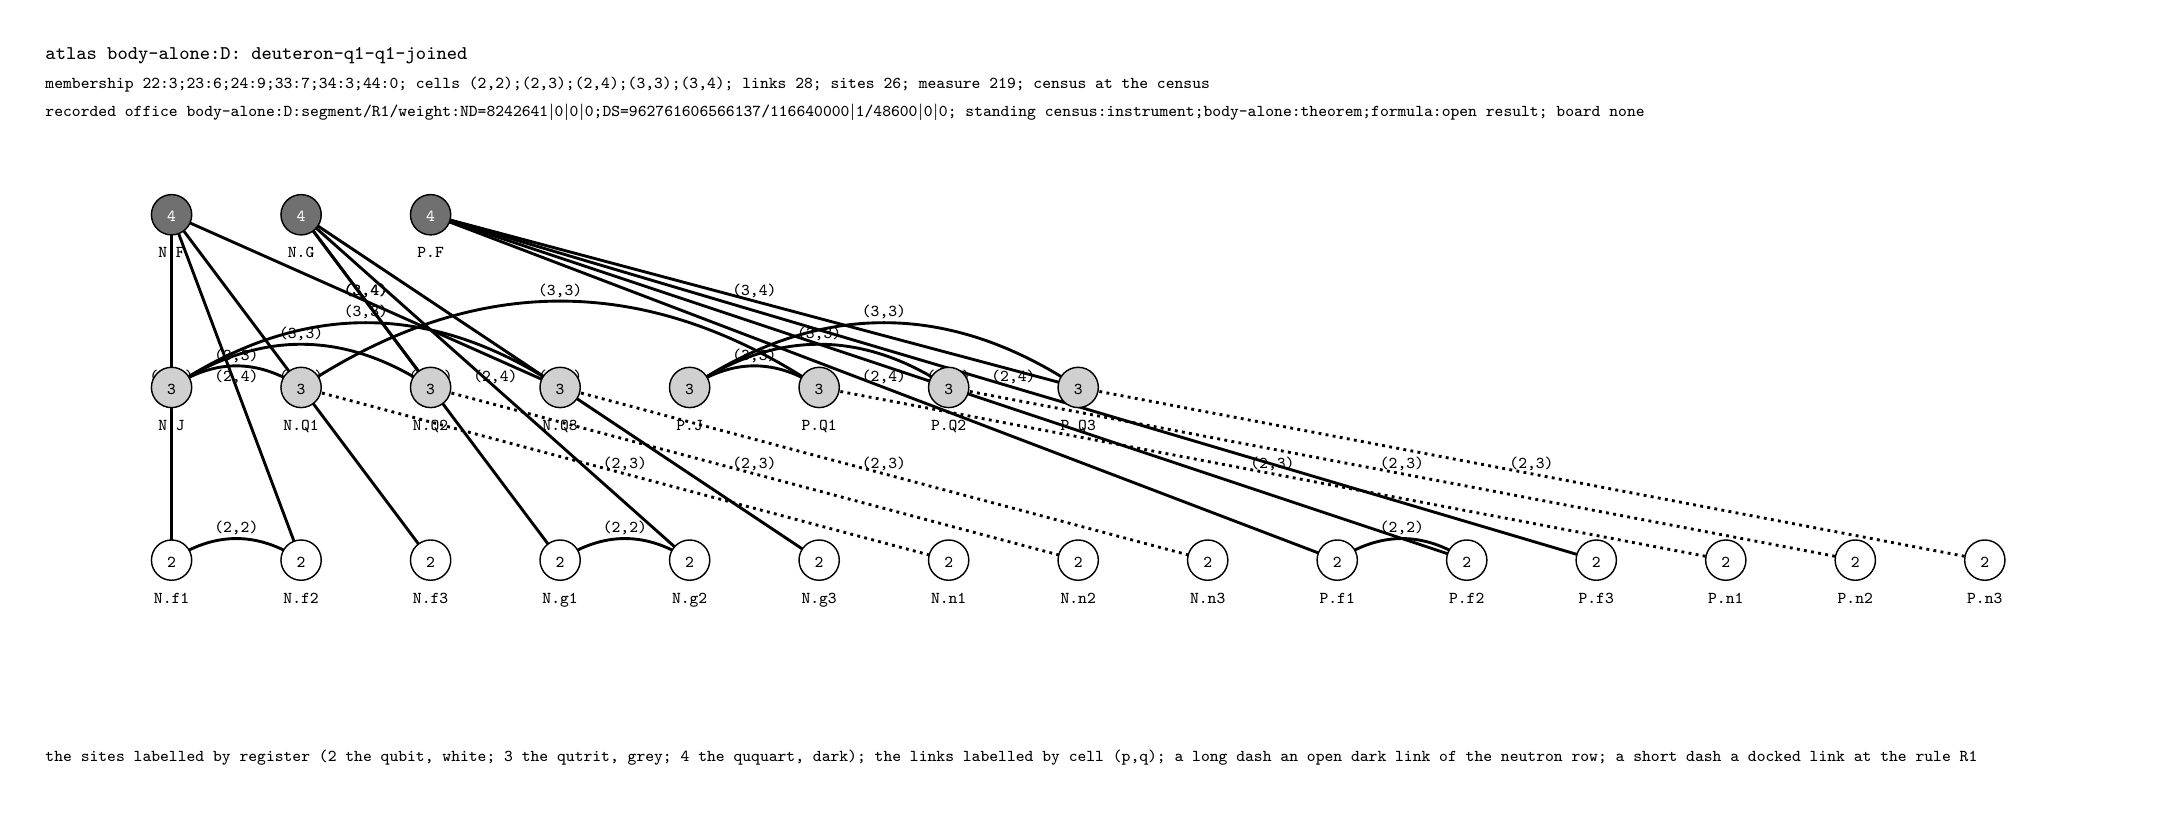
\begin{tikzpicture}[x=0.52pt,y=-0.52pt,baseline]
\clip (0,0) rectangle (1460,540);
\fill[white] (0,0) rectangle (1460,540);
\node[anchor=base west,inner sep=0pt,text=black,font=\fontsize{6.76}{8.112}\selectfont\ttfamily] at (12,22) {atlas body-alone:D: deuteron-q1-q1-joined};
\node[anchor=base west,inner sep=0pt,text=black,font=\fontsize{6.24}{7.488}\selectfont\ttfamily] at (12,42) {membership 22:3;23:6;24:9;33:7;34:3;44:0; cells (2,2);(2,3);(2,4);(3,3);(3,4); links 28; sites 26; measure 219; census at the census};
\node[anchor=base west,inner sep=0pt,text=black,font=\fontsize{5.72}{6.864}\selectfont\ttfamily] at (12,62) {recorded office body-alone:D:segment/R1/weight:ND=8242641\textbar{}0\textbar{}0\textbar{}0;DS=962761606566137/116640000\textbar{}1/48600\textbar{}0\textbar{}0; standing census:instrument;body-alone:theorem;formula:open result; board none};
\draw[draw=black,line width=1.04pt] (100,130) -- (370,250);
\node[anchor=base,inner sep=0pt,text=black,font=\fontsize{5.72}{6.864}\selectfont\ttfamily] at (235,186) {(3,4)};
\draw[draw=black,line width=1.04pt] (100,130) -- (100,370);
\node[anchor=base,inner sep=0pt,text=black,font=\fontsize{5.72}{6.864}\selectfont\ttfamily] at (100,246) {(2,4)};
\draw[draw=black,line width=1.04pt] (100,130) -- (190,370);
\node[anchor=base,inner sep=0pt,text=black,font=\fontsize{5.72}{6.864}\selectfont\ttfamily] at (145,246) {(2,4)};
\draw[draw=black,line width=1.04pt] (100,130) -- (280,370);
\node[anchor=base,inner sep=0pt,text=black,font=\fontsize{5.72}{6.864}\selectfont\ttfamily] at (190,246) {(2,4)};
\draw[draw=black,line width=1.04pt] (190,130) -- (280,250);
\node[anchor=base,inner sep=0pt,text=black,font=\fontsize{5.72}{6.864}\selectfont\ttfamily] at (235,186) {(3,4)};
\draw[draw=black,line width=1.04pt] (190,130) -- (370,370);
\node[anchor=base,inner sep=0pt,text=black,font=\fontsize{5.72}{6.864}\selectfont\ttfamily] at (280,246) {(2,4)};
\draw[draw=black,line width=1.04pt] (190,130) -- (460,370);
\node[anchor=base,inner sep=0pt,text=black,font=\fontsize{5.72}{6.864}\selectfont\ttfamily] at (325,246) {(2,4)};
\draw[draw=black,line width=1.04pt] (190,130) -- (550,370);
\node[anchor=base,inner sep=0pt,text=black,font=\fontsize{5.72}{6.864}\selectfont\ttfamily] at (370,246) {(2,4)};
\draw[draw=black,line width=1.04pt] (100,250) .. controls (130,230) and (160,230) .. (190,250);
\node[anchor=base,inner sep=0pt,text=black,font=\fontsize{5.72}{6.864}\selectfont\ttfamily] at (145,231) {(3,3)};
\draw[draw=black,line width=1.04pt] (100,250) .. controls (160,210) and (220,210) .. (280,250);
\node[anchor=base,inner sep=0pt,text=black,font=\fontsize{5.72}{6.864}\selectfont\ttfamily] at (190,216) {(3,3)};
\draw[draw=black,line width=1.04pt] (100,250) .. controls (190,190) and (280,190) .. (370,250);
\node[anchor=base,inner sep=0pt,text=black,font=\fontsize{5.72}{6.864}\selectfont\ttfamily] at (235,201) {(3,3)};
\draw[draw=black,line width=1.04pt,dash pattern=on 1.04pt off 1.56pt] (190,250) -- (640,370);
\node[anchor=base,inner sep=0pt,text=black,font=\fontsize{5.72}{6.864}\selectfont\ttfamily] at (415,306) {(2,3)};
\draw[draw=black,line width=1.04pt] (190,250) .. controls (310,170) and (430,170) .. (550,250);
\node[anchor=base,inner sep=0pt,text=black,font=\fontsize{5.72}{6.864}\selectfont\ttfamily] at (370,186) {(3,3)};
\draw[draw=black,line width=1.04pt,dash pattern=on 1.04pt off 1.56pt] (280,250) -- (730,370);
\node[anchor=base,inner sep=0pt,text=black,font=\fontsize{5.72}{6.864}\selectfont\ttfamily] at (505,306) {(2,3)};
\draw[draw=black,line width=1.04pt,dash pattern=on 1.04pt off 1.56pt] (370,250) -- (820,370);
\node[anchor=base,inner sep=0pt,text=black,font=\fontsize{5.72}{6.864}\selectfont\ttfamily] at (595,306) {(2,3)};
\draw[draw=black,line width=1.04pt] (100,370) .. controls (130,350) and (160,350) .. (190,370);
\node[anchor=base,inner sep=0pt,text=black,font=\fontsize{5.72}{6.864}\selectfont\ttfamily] at (145,351) {(2,2)};
\draw[draw=black,line width=1.04pt] (370,370) .. controls (400,350) and (430,350) .. (460,370);
\node[anchor=base,inner sep=0pt,text=black,font=\fontsize{5.72}{6.864}\selectfont\ttfamily] at (415,351) {(2,2)};
\draw[draw=black,line width=1.04pt] (280,130) -- (730,250);
\node[anchor=base,inner sep=0pt,text=black,font=\fontsize{5.72}{6.864}\selectfont\ttfamily] at (505,186) {(3,4)};
\draw[draw=black,line width=1.04pt] (280,130) -- (910,370);
\node[anchor=base,inner sep=0pt,text=black,font=\fontsize{5.72}{6.864}\selectfont\ttfamily] at (595,246) {(2,4)};
\draw[draw=black,line width=1.04pt] (280,130) -- (1000,370);
\node[anchor=base,inner sep=0pt,text=black,font=\fontsize{5.72}{6.864}\selectfont\ttfamily] at (640,246) {(2,4)};
\draw[draw=black,line width=1.04pt] (280,130) -- (1090,370);
\node[anchor=base,inner sep=0pt,text=black,font=\fontsize{5.72}{6.864}\selectfont\ttfamily] at (685,246) {(2,4)};
\draw[draw=black,line width=1.04pt] (460,250) .. controls (490,230) and (520,230) .. (550,250);
\node[anchor=base,inner sep=0pt,text=black,font=\fontsize{5.72}{6.864}\selectfont\ttfamily] at (505,231) {(3,3)};
\draw[draw=black,line width=1.04pt] (460,250) .. controls (520,210) and (580,210) .. (640,250);
\node[anchor=base,inner sep=0pt,text=black,font=\fontsize{5.72}{6.864}\selectfont\ttfamily] at (550,216) {(3,3)};
\draw[draw=black,line width=1.04pt] (460,250) .. controls (550,190) and (640,190) .. (730,250);
\node[anchor=base,inner sep=0pt,text=black,font=\fontsize{5.72}{6.864}\selectfont\ttfamily] at (595,201) {(3,3)};
\draw[draw=black,line width=1.04pt,dash pattern=on 1.04pt off 1.56pt] (550,250) -- (1180,370);
\node[anchor=base,inner sep=0pt,text=black,font=\fontsize{5.72}{6.864}\selectfont\ttfamily] at (865,306) {(2,3)};
\draw[draw=black,line width=1.04pt,dash pattern=on 1.04pt off 1.56pt] (640,250) -- (1270,370);
\node[anchor=base,inner sep=0pt,text=black,font=\fontsize{5.72}{6.864}\selectfont\ttfamily] at (955,306) {(2,3)};
\draw[draw=black,line width=1.04pt,dash pattern=on 1.04pt off 1.56pt] (730,250) -- (1360,370);
\node[anchor=base,inner sep=0pt,text=black,font=\fontsize{5.72}{6.864}\selectfont\ttfamily] at (1045,306) {(2,3)};
\draw[draw=black,line width=1.04pt] (910,370) .. controls (940,350) and (970,350) .. (1000,370);
\node[anchor=base,inner sep=0pt,text=black,font=\fontsize{5.72}{6.864}\selectfont\ttfamily] at (955,351) {(2,2)};
\filldraw[fill={rgb,255:red,112;green,112;blue,112},draw=black,line width=0.52pt] (100,130) circle (14);
\node[anchor=base,inner sep=0pt,text=white,font=\fontsize{6.24}{7.488}\selectfont\ttfamily] at (100,135) {4};
\node[anchor=base,inner sep=0pt,text=black,font=\fontsize{5.72}{6.864}\selectfont\ttfamily] at (100,160) {N.F};
\filldraw[fill={rgb,255:red,112;green,112;blue,112},draw=black,line width=0.52pt] (190,130) circle (14);
\node[anchor=base,inner sep=0pt,text=white,font=\fontsize{6.24}{7.488}\selectfont\ttfamily] at (190,135) {4};
\node[anchor=base,inner sep=0pt,text=black,font=\fontsize{5.72}{6.864}\selectfont\ttfamily] at (190,160) {N.G};
\filldraw[fill={rgb,255:red,208;green,208;blue,208},draw=black,line width=0.52pt] (100,250) circle (14);
\node[anchor=base,inner sep=0pt,text=black,font=\fontsize{6.24}{7.488}\selectfont\ttfamily] at (100,255) {3};
\node[anchor=base,inner sep=0pt,text=black,font=\fontsize{5.72}{6.864}\selectfont\ttfamily] at (100,280) {N.J};
\filldraw[fill={rgb,255:red,208;green,208;blue,208},draw=black,line width=0.52pt] (190,250) circle (14);
\node[anchor=base,inner sep=0pt,text=black,font=\fontsize{6.24}{7.488}\selectfont\ttfamily] at (190,255) {3};
\node[anchor=base,inner sep=0pt,text=black,font=\fontsize{5.72}{6.864}\selectfont\ttfamily] at (190,280) {N.Q1};
\filldraw[fill={rgb,255:red,208;green,208;blue,208},draw=black,line width=0.52pt] (280,250) circle (14);
\node[anchor=base,inner sep=0pt,text=black,font=\fontsize{6.24}{7.488}\selectfont\ttfamily] at (280,255) {3};
\node[anchor=base,inner sep=0pt,text=black,font=\fontsize{5.72}{6.864}\selectfont\ttfamily] at (280,280) {N.Q2};
\filldraw[fill={rgb,255:red,208;green,208;blue,208},draw=black,line width=0.52pt] (370,250) circle (14);
\node[anchor=base,inner sep=0pt,text=black,font=\fontsize{6.24}{7.488}\selectfont\ttfamily] at (370,255) {3};
\node[anchor=base,inner sep=0pt,text=black,font=\fontsize{5.72}{6.864}\selectfont\ttfamily] at (370,280) {N.Q3};
\filldraw[fill=white,draw=black,line width=0.52pt] (100,370) circle (14);
\node[anchor=base,inner sep=0pt,text=black,font=\fontsize{6.24}{7.488}\selectfont\ttfamily] at (100,375) {2};
\node[anchor=base,inner sep=0pt,text=black,font=\fontsize{5.72}{6.864}\selectfont\ttfamily] at (100,400) {N.f1};
\filldraw[fill=white,draw=black,line width=0.52pt] (190,370) circle (14);
\node[anchor=base,inner sep=0pt,text=black,font=\fontsize{6.24}{7.488}\selectfont\ttfamily] at (190,375) {2};
\node[anchor=base,inner sep=0pt,text=black,font=\fontsize{5.72}{6.864}\selectfont\ttfamily] at (190,400) {N.f2};
\filldraw[fill=white,draw=black,line width=0.52pt] (280,370) circle (14);
\node[anchor=base,inner sep=0pt,text=black,font=\fontsize{6.24}{7.488}\selectfont\ttfamily] at (280,375) {2};
\node[anchor=base,inner sep=0pt,text=black,font=\fontsize{5.72}{6.864}\selectfont\ttfamily] at (280,400) {N.f3};
\filldraw[fill=white,draw=black,line width=0.52pt] (370,370) circle (14);
\node[anchor=base,inner sep=0pt,text=black,font=\fontsize{6.24}{7.488}\selectfont\ttfamily] at (370,375) {2};
\node[anchor=base,inner sep=0pt,text=black,font=\fontsize{5.72}{6.864}\selectfont\ttfamily] at (370,400) {N.g1};
\filldraw[fill=white,draw=black,line width=0.52pt] (460,370) circle (14);
\node[anchor=base,inner sep=0pt,text=black,font=\fontsize{6.24}{7.488}\selectfont\ttfamily] at (460,375) {2};
\node[anchor=base,inner sep=0pt,text=black,font=\fontsize{5.72}{6.864}\selectfont\ttfamily] at (460,400) {N.g2};
\filldraw[fill=white,draw=black,line width=0.52pt] (550,370) circle (14);
\node[anchor=base,inner sep=0pt,text=black,font=\fontsize{6.24}{7.488}\selectfont\ttfamily] at (550,375) {2};
\node[anchor=base,inner sep=0pt,text=black,font=\fontsize{5.72}{6.864}\selectfont\ttfamily] at (550,400) {N.g3};
\filldraw[fill=white,draw=black,line width=0.52pt] (640,370) circle (14);
\node[anchor=base,inner sep=0pt,text=black,font=\fontsize{6.24}{7.488}\selectfont\ttfamily] at (640,375) {2};
\node[anchor=base,inner sep=0pt,text=black,font=\fontsize{5.72}{6.864}\selectfont\ttfamily] at (640,400) {N.n1};
\filldraw[fill=white,draw=black,line width=0.52pt] (730,370) circle (14);
\node[anchor=base,inner sep=0pt,text=black,font=\fontsize{6.24}{7.488}\selectfont\ttfamily] at (730,375) {2};
\node[anchor=base,inner sep=0pt,text=black,font=\fontsize{5.72}{6.864}\selectfont\ttfamily] at (730,400) {N.n2};
\filldraw[fill=white,draw=black,line width=0.52pt] (820,370) circle (14);
\node[anchor=base,inner sep=0pt,text=black,font=\fontsize{6.24}{7.488}\selectfont\ttfamily] at (820,375) {2};
\node[anchor=base,inner sep=0pt,text=black,font=\fontsize{5.72}{6.864}\selectfont\ttfamily] at (820,400) {N.n3};
\filldraw[fill={rgb,255:red,112;green,112;blue,112},draw=black,line width=0.52pt] (280,130) circle (14);
\node[anchor=base,inner sep=0pt,text=white,font=\fontsize{6.24}{7.488}\selectfont\ttfamily] at (280,135) {4};
\node[anchor=base,inner sep=0pt,text=black,font=\fontsize{5.72}{6.864}\selectfont\ttfamily] at (280,160) {P.F};
\filldraw[fill={rgb,255:red,208;green,208;blue,208},draw=black,line width=0.52pt] (460,250) circle (14);
\node[anchor=base,inner sep=0pt,text=black,font=\fontsize{6.24}{7.488}\selectfont\ttfamily] at (460,255) {3};
\node[anchor=base,inner sep=0pt,text=black,font=\fontsize{5.72}{6.864}\selectfont\ttfamily] at (460,280) {P.J};
\filldraw[fill={rgb,255:red,208;green,208;blue,208},draw=black,line width=0.52pt] (550,250) circle (14);
\node[anchor=base,inner sep=0pt,text=black,font=\fontsize{6.24}{7.488}\selectfont\ttfamily] at (550,255) {3};
\node[anchor=base,inner sep=0pt,text=black,font=\fontsize{5.72}{6.864}\selectfont\ttfamily] at (550,280) {P.Q1};
\filldraw[fill={rgb,255:red,208;green,208;blue,208},draw=black,line width=0.52pt] (640,250) circle (14);
\node[anchor=base,inner sep=0pt,text=black,font=\fontsize{6.24}{7.488}\selectfont\ttfamily] at (640,255) {3};
\node[anchor=base,inner sep=0pt,text=black,font=\fontsize{5.72}{6.864}\selectfont\ttfamily] at (640,280) {P.Q2};
\filldraw[fill={rgb,255:red,208;green,208;blue,208},draw=black,line width=0.52pt] (730,250) circle (14);
\node[anchor=base,inner sep=0pt,text=black,font=\fontsize{6.24}{7.488}\selectfont\ttfamily] at (730,255) {3};
\node[anchor=base,inner sep=0pt,text=black,font=\fontsize{5.72}{6.864}\selectfont\ttfamily] at (730,280) {P.Q3};
\filldraw[fill=white,draw=black,line width=0.52pt] (910,370) circle (14);
\node[anchor=base,inner sep=0pt,text=black,font=\fontsize{6.24}{7.488}\selectfont\ttfamily] at (910,375) {2};
\node[anchor=base,inner sep=0pt,text=black,font=\fontsize{5.72}{6.864}\selectfont\ttfamily] at (910,400) {P.f1};
\filldraw[fill=white,draw=black,line width=0.52pt] (1000,370) circle (14);
\node[anchor=base,inner sep=0pt,text=black,font=\fontsize{6.24}{7.488}\selectfont\ttfamily] at (1000,375) {2};
\node[anchor=base,inner sep=0pt,text=black,font=\fontsize{5.72}{6.864}\selectfont\ttfamily] at (1000,400) {P.f2};
\filldraw[fill=white,draw=black,line width=0.52pt] (1090,370) circle (14);
\node[anchor=base,inner sep=0pt,text=black,font=\fontsize{6.24}{7.488}\selectfont\ttfamily] at (1090,375) {2};
\node[anchor=base,inner sep=0pt,text=black,font=\fontsize{5.72}{6.864}\selectfont\ttfamily] at (1090,400) {P.f3};
\filldraw[fill=white,draw=black,line width=0.52pt] (1180,370) circle (14);
\node[anchor=base,inner sep=0pt,text=black,font=\fontsize{6.24}{7.488}\selectfont\ttfamily] at (1180,375) {2};
\node[anchor=base,inner sep=0pt,text=black,font=\fontsize{5.72}{6.864}\selectfont\ttfamily] at (1180,400) {P.n1};
\filldraw[fill=white,draw=black,line width=0.52pt] (1270,370) circle (14);
\node[anchor=base,inner sep=0pt,text=black,font=\fontsize{6.24}{7.488}\selectfont\ttfamily] at (1270,375) {2};
\node[anchor=base,inner sep=0pt,text=black,font=\fontsize{5.72}{6.864}\selectfont\ttfamily] at (1270,400) {P.n2};
\filldraw[fill=white,draw=black,line width=0.52pt] (1360,370) circle (14);
\node[anchor=base,inner sep=0pt,text=black,font=\fontsize{6.24}{7.488}\selectfont\ttfamily] at (1360,375) {2};
\node[anchor=base,inner sep=0pt,text=black,font=\fontsize{5.72}{6.864}\selectfont\ttfamily] at (1360,400) {P.n3};
\node[anchor=base west,inner sep=0pt,text=black,font=\fontsize{5.72}{6.864}\selectfont\ttfamily] at (12,510) {the sites labelled by register (2 the qubit, white; 3 the qutrit, grey; 4 the ququart, dark); the links labelled by cell (p,q); a long dash an open dark link of the neutron row; a short dash a docked link at the rule R1};
\end{tikzpicture}\end{adjustbox}
\caption{\texttt{deuteron-q1-q1-joined}, deuteron joined: 26 sites, 28 links, the measure 219; the links at the cells (2,2), (2,3), (2,4), (3,3), (3,4); the membership 22:3; 23:6; 24:9; 33:7; 34:3; 44:0; 6 docked links at the rule R1 (P.Q1-P.n1; P.Q2-P.n2; P.Q3-P.n3; N.Q1-N.n1; N.Q2-N.n2; N.Q3-N.n3); at the census of the six cells. Drawn at the anatomy atlas as its web, the sites labeled by register and the links by cell, from the the body-alone office rule.}\label{fig:VIII-2-D537322-deuteron-q1-q1-joined-b6dadc}
\begin{center}\footnotesize\begin{adjustbox}{max width=\linewidth}\begin{tabular}{p{0.26\textwidth}p{0.68\textwidth}}\toprule
recorded office (the slot-count row) & the read o-nd of the formula row: the first power 2871; the office \texttt{8242641\textbar{}0\textbar{}0\textbar{}0}; against the formula with the slot count equal; the slot total 0; dark links 22; hubs P.F; N.F; N.G; dressing 9 \\
mass register (the mass-register row) & the read BD: the class touching the ququart; the first power 4941; the office \texttt{15 999 659 899 116 267/655360000\textbar{}1983/50\textbar{}14163873/32768000\textbar{}0}; nonzero; met yes; hubs N.F; N.G; P.F; in-legs P.Q3-P.F; N.Q3-N.F; N.Q2-N.G; dressing 27; ports P.Q1-P.n1; P.Q2-P.n2; P.Q3-P.n3; P.f-p.f3; N.Q1-N.n1; N.Q2-N.n2; N.Q3-N.n3; N.f-n.f3; N.g-n.g3 \\
junction registers (the hadron row) & the read ND: junctions P.J; P.Q1; P.Q3; N.J; N.Q1; N.Q2; N.Q3; the share one third per leg; the registers at the share 219, struck 183, mono 5913, the hub spelling 1971; against the cells none; none; none; none, none \\
\bottomrule\end{tabular}\end{adjustbox}\end{center}
\end{figure}
\begin{figure}[H]\centering
\begin{adjustbox}{max width=\linewidth}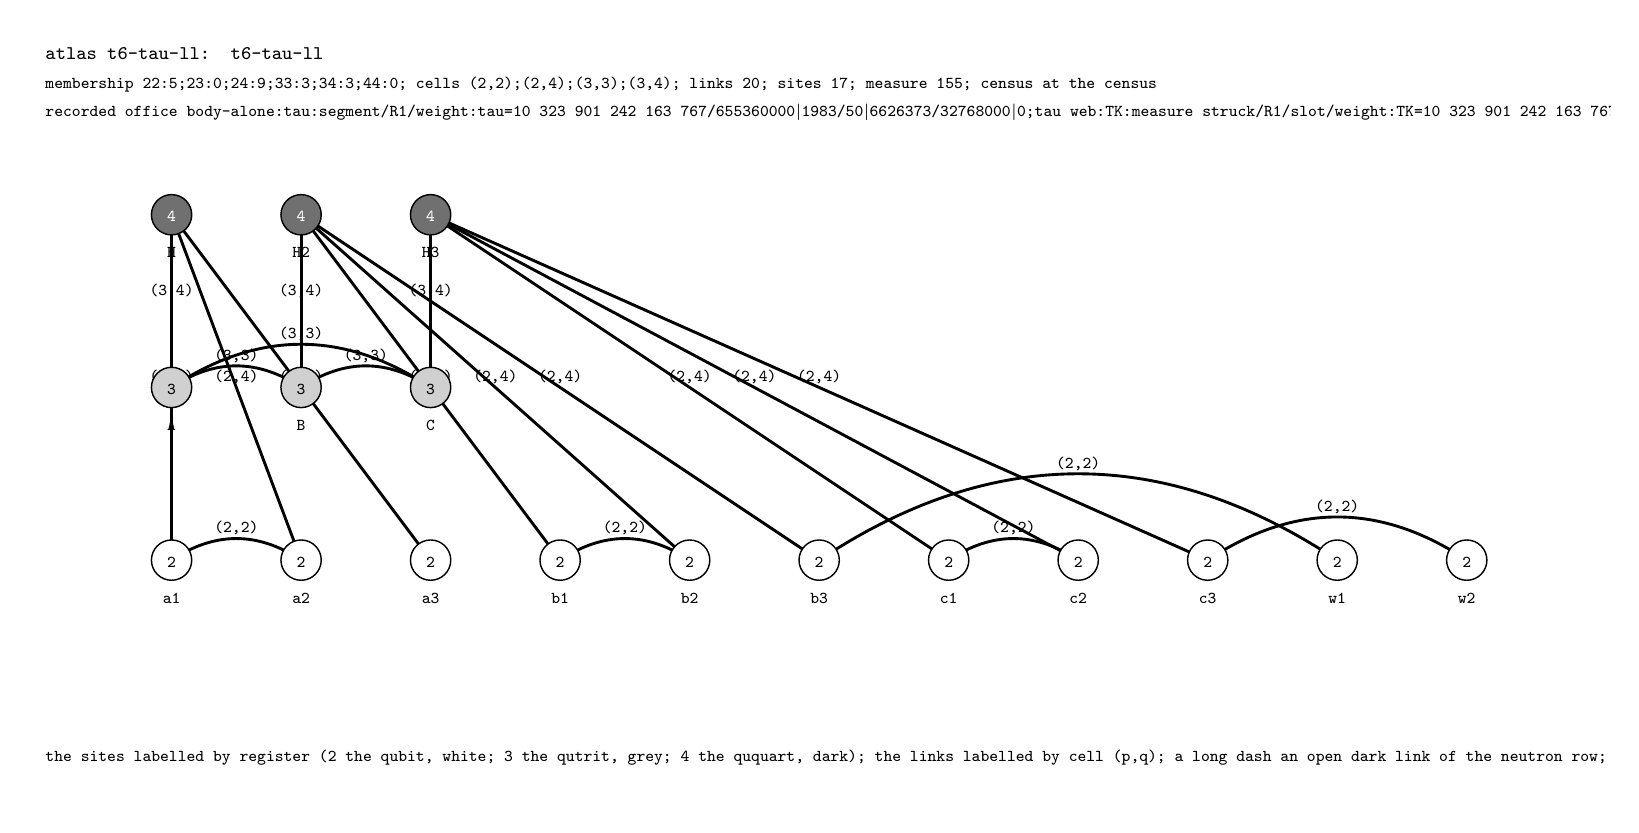
\begin{tikzpicture}[x=0.52pt,y=-0.52pt,baseline]
\clip (0,0) rectangle (1100,540);
\fill[white] (0,0) rectangle (1100,540);
\node[anchor=base west,inner sep=0pt,text=black,font=\fontsize{6.76}{8.112}\selectfont\ttfamily] at (12,22) {atlas t6-tau-ll: t6-tau-ll};
\node[anchor=base west,inner sep=0pt,text=black,font=\fontsize{6.24}{7.488}\selectfont\ttfamily] at (12,42) {membership 22:5;23:0;24:9;33:3;34:3;44:0; cells (2,2);(2,4);(3,3);(3,4); links 20; sites 17; measure 155; census at the census};
\node[anchor=base west,inner sep=0pt,text=black,font=\fontsize{5.72}{6.864}\selectfont\ttfamily] at (12,62) {recorded office body-alone:tau:segment/R1/weight:tau=10 323 901 242 163 767/655360000\textbar{}1983/50\textbar{}6626373/32768000\textbar{}0;tau web:TK:measure struck/R1/slot/weight:TK=10 323 901 242 163 767/655360000\textbar{}1983/50\textbar{}6626373/32768000\textbar{}0; standing census:instrument;body-alone:theorem;formula:open result;tau web:theorem;roster:roster word; board tau};
\draw[draw=black,line width=1.04pt] (100,250) .. controls (130,230) and (160,230) .. (190,250);
\node[anchor=base,inner sep=0pt,text=black,font=\fontsize{5.72}{6.864}\selectfont\ttfamily] at (145,231) {(3,3)};
\draw[draw=black,line width=1.04pt] (100,250) .. controls (160,210) and (220,210) .. (280,250);
\node[anchor=base,inner sep=0pt,text=black,font=\fontsize{5.72}{6.864}\selectfont\ttfamily] at (190,216) {(3,3)};
\draw[draw=black,line width=1.04pt] (100,250) -- (100,130);
\node[anchor=base,inner sep=0pt,text=black,font=\fontsize{5.72}{6.864}\selectfont\ttfamily] at (100,186) {(3,4)};
\draw[draw=black,line width=1.04pt] (190,250) .. controls (220,230) and (250,230) .. (280,250);
\node[anchor=base,inner sep=0pt,text=black,font=\fontsize{5.72}{6.864}\selectfont\ttfamily] at (235,231) {(3,3)};
\draw[draw=black,line width=1.04pt] (190,250) -- (190,130);
\node[anchor=base,inner sep=0pt,text=black,font=\fontsize{5.72}{6.864}\selectfont\ttfamily] at (190,186) {(3,4)};
\draw[draw=black,line width=1.04pt] (280,250) -- (280,130);
\node[anchor=base,inner sep=0pt,text=black,font=\fontsize{5.72}{6.864}\selectfont\ttfamily] at (280,186) {(3,4)};
\draw[draw=black,line width=1.04pt] (100,130) -- (100,370);
\node[anchor=base,inner sep=0pt,text=black,font=\fontsize{5.72}{6.864}\selectfont\ttfamily] at (100,246) {(2,4)};
\draw[draw=black,line width=1.04pt] (100,130) -- (190,370);
\node[anchor=base,inner sep=0pt,text=black,font=\fontsize{5.72}{6.864}\selectfont\ttfamily] at (145,246) {(2,4)};
\draw[draw=black,line width=1.04pt] (100,130) -- (280,370);
\node[anchor=base,inner sep=0pt,text=black,font=\fontsize{5.72}{6.864}\selectfont\ttfamily] at (190,246) {(2,4)};
\draw[draw=black,line width=1.04pt] (190,130) -- (370,370);
\node[anchor=base,inner sep=0pt,text=black,font=\fontsize{5.72}{6.864}\selectfont\ttfamily] at (280,246) {(2,4)};
\draw[draw=black,line width=1.04pt] (190,130) -- (460,370);
\node[anchor=base,inner sep=0pt,text=black,font=\fontsize{5.72}{6.864}\selectfont\ttfamily] at (325,246) {(2,4)};
\draw[draw=black,line width=1.04pt] (190,130) -- (550,370);
\node[anchor=base,inner sep=0pt,text=black,font=\fontsize{5.72}{6.864}\selectfont\ttfamily] at (370,246) {(2,4)};
\draw[draw=black,line width=1.04pt] (280,130) -- (640,370);
\node[anchor=base,inner sep=0pt,text=black,font=\fontsize{5.72}{6.864}\selectfont\ttfamily] at (460,246) {(2,4)};
\draw[draw=black,line width=1.04pt] (280,130) -- (730,370);
\node[anchor=base,inner sep=0pt,text=black,font=\fontsize{5.72}{6.864}\selectfont\ttfamily] at (505,246) {(2,4)};
\draw[draw=black,line width=1.04pt] (280,130) -- (820,370);
\node[anchor=base,inner sep=0pt,text=black,font=\fontsize{5.72}{6.864}\selectfont\ttfamily] at (550,246) {(2,4)};
\draw[draw=black,line width=1.04pt] (100,370) .. controls (130,350) and (160,350) .. (190,370);
\node[anchor=base,inner sep=0pt,text=black,font=\fontsize{5.72}{6.864}\selectfont\ttfamily] at (145,351) {(2,2)};
\draw[draw=black,line width=1.04pt] (370,370) .. controls (400,350) and (430,350) .. (460,370);
\node[anchor=base,inner sep=0pt,text=black,font=\fontsize{5.72}{6.864}\selectfont\ttfamily] at (415,351) {(2,2)};
\draw[draw=black,line width=1.04pt] (550,370) .. controls (670,290) and (790,290) .. (910,370);
\node[anchor=base,inner sep=0pt,text=black,font=\fontsize{5.72}{6.864}\selectfont\ttfamily] at (730,306) {(2,2)};
\draw[draw=black,line width=1.04pt] (640,370) .. controls (670,350) and (700,350) .. (730,370);
\node[anchor=base,inner sep=0pt,text=black,font=\fontsize{5.72}{6.864}\selectfont\ttfamily] at (685,351) {(2,2)};
\draw[draw=black,line width=1.04pt] (820,370) .. controls (880,330) and (940,330) .. (1000,370);
\node[anchor=base,inner sep=0pt,text=black,font=\fontsize{5.72}{6.864}\selectfont\ttfamily] at (910,336) {(2,2)};
\filldraw[fill={rgb,255:red,208;green,208;blue,208},draw=black,line width=0.52pt] (100,250) circle (14);
\node[anchor=base,inner sep=0pt,text=black,font=\fontsize{6.24}{7.488}\selectfont\ttfamily] at (100,255) {3};
\node[anchor=base,inner sep=0pt,text=black,font=\fontsize{5.72}{6.864}\selectfont\ttfamily] at (100,280) {A};
\filldraw[fill={rgb,255:red,208;green,208;blue,208},draw=black,line width=0.52pt] (190,250) circle (14);
\node[anchor=base,inner sep=0pt,text=black,font=\fontsize{6.24}{7.488}\selectfont\ttfamily] at (190,255) {3};
\node[anchor=base,inner sep=0pt,text=black,font=\fontsize{5.72}{6.864}\selectfont\ttfamily] at (190,280) {B};
\filldraw[fill={rgb,255:red,208;green,208;blue,208},draw=black,line width=0.52pt] (280,250) circle (14);
\node[anchor=base,inner sep=0pt,text=black,font=\fontsize{6.24}{7.488}\selectfont\ttfamily] at (280,255) {3};
\node[anchor=base,inner sep=0pt,text=black,font=\fontsize{5.72}{6.864}\selectfont\ttfamily] at (280,280) {C};
\filldraw[fill={rgb,255:red,112;green,112;blue,112},draw=black,line width=0.52pt] (100,130) circle (14);
\node[anchor=base,inner sep=0pt,text=white,font=\fontsize{6.24}{7.488}\selectfont\ttfamily] at (100,135) {4};
\node[anchor=base,inner sep=0pt,text=black,font=\fontsize{5.72}{6.864}\selectfont\ttfamily] at (100,160) {H};
\filldraw[fill={rgb,255:red,112;green,112;blue,112},draw=black,line width=0.52pt] (190,130) circle (14);
\node[anchor=base,inner sep=0pt,text=white,font=\fontsize{6.24}{7.488}\selectfont\ttfamily] at (190,135) {4};
\node[anchor=base,inner sep=0pt,text=black,font=\fontsize{5.72}{6.864}\selectfont\ttfamily] at (190,160) {H2};
\filldraw[fill={rgb,255:red,112;green,112;blue,112},draw=black,line width=0.52pt] (280,130) circle (14);
\node[anchor=base,inner sep=0pt,text=white,font=\fontsize{6.24}{7.488}\selectfont\ttfamily] at (280,135) {4};
\node[anchor=base,inner sep=0pt,text=black,font=\fontsize{5.72}{6.864}\selectfont\ttfamily] at (280,160) {H3};
\filldraw[fill=white,draw=black,line width=0.52pt] (100,370) circle (14);
\node[anchor=base,inner sep=0pt,text=black,font=\fontsize{6.24}{7.488}\selectfont\ttfamily] at (100,375) {2};
\node[anchor=base,inner sep=0pt,text=black,font=\fontsize{5.72}{6.864}\selectfont\ttfamily] at (100,400) {a1};
\filldraw[fill=white,draw=black,line width=0.52pt] (190,370) circle (14);
\node[anchor=base,inner sep=0pt,text=black,font=\fontsize{6.24}{7.488}\selectfont\ttfamily] at (190,375) {2};
\node[anchor=base,inner sep=0pt,text=black,font=\fontsize{5.72}{6.864}\selectfont\ttfamily] at (190,400) {a2};
\filldraw[fill=white,draw=black,line width=0.52pt] (280,370) circle (14);
\node[anchor=base,inner sep=0pt,text=black,font=\fontsize{6.24}{7.488}\selectfont\ttfamily] at (280,375) {2};
\node[anchor=base,inner sep=0pt,text=black,font=\fontsize{5.72}{6.864}\selectfont\ttfamily] at (280,400) {a3};
\filldraw[fill=white,draw=black,line width=0.52pt] (370,370) circle (14);
\node[anchor=base,inner sep=0pt,text=black,font=\fontsize{6.24}{7.488}\selectfont\ttfamily] at (370,375) {2};
\node[anchor=base,inner sep=0pt,text=black,font=\fontsize{5.72}{6.864}\selectfont\ttfamily] at (370,400) {b1};
\filldraw[fill=white,draw=black,line width=0.52pt] (460,370) circle (14);
\node[anchor=base,inner sep=0pt,text=black,font=\fontsize{6.24}{7.488}\selectfont\ttfamily] at (460,375) {2};
\node[anchor=base,inner sep=0pt,text=black,font=\fontsize{5.72}{6.864}\selectfont\ttfamily] at (460,400) {b2};
\filldraw[fill=white,draw=black,line width=0.52pt] (550,370) circle (14);
\node[anchor=base,inner sep=0pt,text=black,font=\fontsize{6.24}{7.488}\selectfont\ttfamily] at (550,375) {2};
\node[anchor=base,inner sep=0pt,text=black,font=\fontsize{5.72}{6.864}\selectfont\ttfamily] at (550,400) {b3};
\filldraw[fill=white,draw=black,line width=0.52pt] (640,370) circle (14);
\node[anchor=base,inner sep=0pt,text=black,font=\fontsize{6.24}{7.488}\selectfont\ttfamily] at (640,375) {2};
\node[anchor=base,inner sep=0pt,text=black,font=\fontsize{5.72}{6.864}\selectfont\ttfamily] at (640,400) {c1};
\filldraw[fill=white,draw=black,line width=0.52pt] (730,370) circle (14);
\node[anchor=base,inner sep=0pt,text=black,font=\fontsize{6.24}{7.488}\selectfont\ttfamily] at (730,375) {2};
\node[anchor=base,inner sep=0pt,text=black,font=\fontsize{5.72}{6.864}\selectfont\ttfamily] at (730,400) {c2};
\filldraw[fill=white,draw=black,line width=0.52pt] (820,370) circle (14);
\node[anchor=base,inner sep=0pt,text=black,font=\fontsize{6.24}{7.488}\selectfont\ttfamily] at (820,375) {2};
\node[anchor=base,inner sep=0pt,text=black,font=\fontsize{5.72}{6.864}\selectfont\ttfamily] at (820,400) {c3};
\filldraw[fill=white,draw=black,line width=0.52pt] (910,370) circle (14);
\node[anchor=base,inner sep=0pt,text=black,font=\fontsize{6.24}{7.488}\selectfont\ttfamily] at (910,375) {2};
\node[anchor=base,inner sep=0pt,text=black,font=\fontsize{5.72}{6.864}\selectfont\ttfamily] at (910,400) {w1};
\filldraw[fill=white,draw=black,line width=0.52pt] (1000,370) circle (14);
\node[anchor=base,inner sep=0pt,text=black,font=\fontsize{6.24}{7.488}\selectfont\ttfamily] at (1000,375) {2};
\node[anchor=base,inner sep=0pt,text=black,font=\fontsize{5.72}{6.864}\selectfont\ttfamily] at (1000,400) {w2};
\node[anchor=base west,inner sep=0pt,text=black,font=\fontsize{5.72}{6.864}\selectfont\ttfamily] at (12,510) {the sites labelled by register (2 the qubit, white; 3 the qutrit, grey; 4 the ququart, dark); the links labelled by cell (p,q); a long dash an open dark link of the neutron row; a short dash a docked link at the rule R1};
\end{tikzpicture}\end{adjustbox}
\caption{\texttt{t6-tau-ll} (the tau), recorded body, roster web: 17 sites, 20 links, the measure 155; the links at the cells (2,2), (2,4), (3,3), (3,4); the membership 22:5; 23:0; 24:9; 33:3; 34:3; 44:0; dock-free at the rule R1; at the census of the six cells. Drawn at the anatomy atlas as its web, the sites labeled by register and the links by cell, from the the body-alone office rule.}\label{fig:VIII-2-D537322-t6-tau-ll-cfed05}
\begin{center}\footnotesize\begin{adjustbox}{max width=\linewidth}\begin{tabular}{p{0.26\textwidth}p{0.68\textwidth}}\toprule
recorded office (the slot-count row) & the read o-tau of the formula row: the first power 3969; the office \texttt{10 323 901 242 163 767/655360000\textbar{}1983/50\textbar{}6626373/32768000\textbar{}0}; against the formula with the slot count equal; the slot total 0; dark links 20; hubs H; H2; H3; dressing 27 \\
mass register (the mass-register row) & the read btau: the class touching the ququart; the first power 3969; the office \texttt{10 323 901 242 163 767/655360000\textbar{}1983/50\textbar{}6626373/32768000\textbar{}0}; nonzero; met yes; hubs H; H2; H3; in-legs h-a; H2-B; H3-C; dressing 27; ports H-a3; w1-b3; w2-c3 \\
lepton-form office (the lepton row) & the read l-tk: the first power 3969; the office \texttt{10 323 901 242 163 767/655360000\textbar{}1983/50\textbar{}6626373/32768000\textbar{}0}; against the cell equal; dark links 20 \\
\bottomrule\end{tabular}\end{adjustbox}\end{center}
\end{figure}
\begin{figure}[h]
\centering
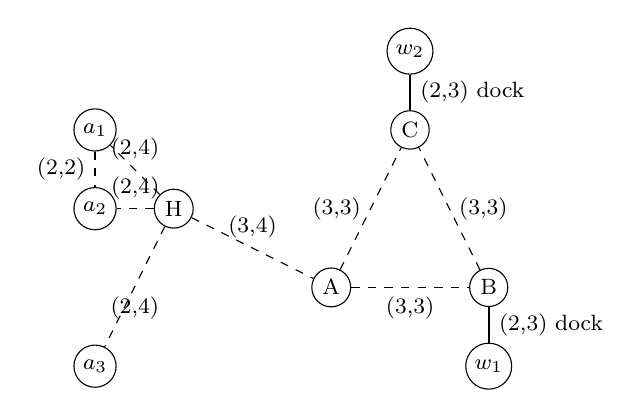
\begin{tikzpicture}[every node/.style={font=\footnotesize}]
\node[circle,draw,inner sep=2pt] (A) at (0,0) {A};
\node[circle,draw,inner sep=2pt] (B) at (2,0) {B};
\node[circle,draw,inner sep=2pt] (C) at (1,2) {C};
\node[circle,draw,inner sep=2pt] (H) at (-2,1) {H};
\node[circle,draw,inner sep=2pt] (a1) at (-3,2) {$a_1$};
\node[circle,draw,inner sep=2pt] (a2) at (-3,1) {$a_2$};
\node[circle,draw,inner sep=2pt] (a3) at (-3,-1) {$a_3$};
\node[circle,draw,inner sep=2pt] (w1) at (2,-1) {$w_1$};
\node[circle,draw,inner sep=2pt] (w2) at (1,3) {$w_2$};
\draw[dashed] (A) -- node[below] {(3,3)} (B);
\draw[dashed] (B) -- node[right] {(3,3)} (C);
\draw[dashed] (A) -- node[left] {(3,3)} (C);
\draw[dashed] (H) -- node[above] {(3,4)} (A);
\draw[dashed] (H) -- node[above] {(2,4)} (a1);
\draw[dashed] (H) -- node[above] {(2,4)} (a2);
\draw[dashed] (H) -- node[below] {(2,4)} (a3);
\draw[dashed] (a1) -- node[left] {(2,2)} (a2);
\draw[thick] (B) -- node[right] {(2,3) dock} (w1);
\draw[thick] (C) -- node[right] {(2,3) dock} (w2);
\end{tikzpicture}
\caption{The two-dock electron web of the body-alone rule. Nine sites and ten links, each link labeled by its genre. The two (2,3) docks at $w_1$ and $w_2$ carry the read, and the eight dashed links of the other genres form the dark set that closes at the closure term.}
\end{figure}
\par\medskip\noindent{\itshape Beyond the first power, the next chapter reads the next terms.}\label{narr:close:8-2}\par
\section{The next terms and the unstable rows}\label{mod:VIII-3-next-terms-and-the-unstable-rows}
\chdesig{10-3}{8-3}{VIII-3-next-terms-and-the-unstable-rows}{VIII-3-next-terms-and-the-unstable-rows}
\label{narr:open:8-3}Theorem~196.1 reads the next terms and the unstable rows, and Theorem~196.2, a theorem, the lepton joined face at the open attach site.
\begin{chconditional}[The next terms and the unstable rows]\label{box:VIII-3-next-terms-and-the-unstable-rows:1}
Conditional on the results this entry rests on, among them first power as the act readout sum and mass as the direct two-exchange sum at the common support, each at its own standing. At the cells of the ladder, the link-weight placement and the dock spelling, with the unit the dock-struck electron first power, every next term is an exact object with a definite sign: positive at the muon office and at the tau office and negative at the Koide relation, the next term at the muon office the closure object over the unit squared, an element of the field of the two roots.
\end{chconditional}
\chstanding{conditional theorem}
\chdeps{Definitions 1.1 to 1.6, Theorem 152.1 and Theorems 185.1 to 185.12}{Open result 157.1 and Theorems 162.1 and 162.2}
\begin{chtheorem}[The lepton joined face at the open attach site]\label{box:VIII-3-next-terms-and-the-unstable-rows:2}
Every site of the tau is typed under the definition of open, the far end of the entered link open exactly when the near end is the larger: twelve of the seventeen sites are open attach sites, and the joined face of the tau is defined at one of them, the body alone at the first order and the second-order object an exact element of the field.
\end{chtheorem}
\chstanding{theorem}
\chdeps{Definitions 1.1 to 1.6, Theorem 152.1 and Theorems 185.1 to 185.12}{Open result 157.1 and Theorems 162.1 and 162.2}
The next term is computed at the link-weight placement at every cell of the ladder at the dock spelling, and its sign is decided exactly through the subfield of the first root. Every site of the tau is typed at the definition of open with the transport-pair table re-met at the dimension rule, and the joined face is taken at an open site. The one open question of the chapter, the unstable-row correction as the open-move readout, is a reading that was tried and parted at its named step, and the object the decay releases stands at its own chapter.
\begin{chbridge}
In quantum field theory the mass of a body is corrected order by order by its self-energy, the next term of the expansion a loop integral with a definite sign at each order \cite{Weinberg1995}, and an unstable body carries a width beside its mass, the pole of its propagator moved off the real axis by the open decay channels \cite{BreitWigner1936}. The correspondence is by name.
\end{chbridge}
\begin{chproof}[exhaustive census with its exact part]
\textit{The premises.} The axiom and the six definitions of Section~\ref{mod:FRAMEWORK}, definitions. The first power and the placement per web of Section~\ref{mod:VIII-1-mass-unit-and-the-first-power}, theorems. The lepton ladder as hub assemblies of Section~\ref{mod:V-10-lepton-ladder-as-hub-assemblies}, a theorem. The Koide reading at the dock unit and the next-term reading, two open readings consumed at their tables. The chain from the axiom to this result is seven chapters deep.

\textit{The exact part: the next term at an office.} The unit is the dock-struck electron first power, $u=67$, re-met at eleven cells of the results above. At a lepton body with the first power $S_1$ and the direct two-exchange sum $S_2$, from the direct sum and the first power, by subtraction, we obtain the closure object $S_2-S_1^{2}$. From the first power and the unit, by division, we obtain the first-order office $S_1^{2}/u^{2}$. From the closure object and the unit, by division, we obtain the next term
\begin{equation}
n=\frac{S_2-S_1^{2}}{u^{2}} ,
\end{equation}
an element of the ring with basis one, root two and root three. From the first-order office and the next term, by addition, we obtain the order-two office $S_2/u^{2}$. The smallest instance is the electron at its own unit. The first-order office is $1$ and the next term is the closure ratio of the first-power result,
\begin{equation}
n_{e}=\tfrac{13\,708\,610\,839}{2\,144\,653\,148\,160\,000}+\tfrac{661}{163\,624\,050}\sqrt{2}+\tfrac{5\,977\,541}{107\,232\,657\,408\,000}\sqrt{3},
\end{equation}
positive. At the muon, against the first-order office $927\,369/4489$, the next term is
\begin{equation}
n_{\mu}=\tfrac{39\,502\,907\,303}{26\,477\,199\,360\,000}+\tfrac{649}{673\,350}\sqrt{2}+\tfrac{6\,301\,957}{1\,323\,859\,968\,000}\sqrt{3},
\end{equation}
and at the tau, against $15\,752\,961/4489$,
\begin{equation}
n_{\tau}=\tfrac{65\,297\,203\,767}{2\,941\,911\,040\,000}+\tfrac{3233}{224\,450}\sqrt{2}+\tfrac{6\,626\,373}{147\,095\,552\,000}\sqrt{3},
\end{equation}
each positive, the sign certified by an exact bracket at forty digits that excludes zero. The order-two offices equal the direct sums over the unit squared of the first-power result at the three bodies. At the Koide relation the three dock-spelled direct sums have roots outside the field of the two roots (none of three in the field, decided exactly through the subfield of root two), the three adjoined roots independent, so the relation is an exact object of the formal tower less the first-order relation $16\,684\,819/24\,990\,001$, whose departure from two thirds, $74\,455/74\,970\,003$, is positive. Its next term is negative, the direct bracket
\begin{equation}
-\tfrac{1\,567\,258\,759\,542\,141\,982\,137\,839\,353\,220\,402}{10^{40}}\ \text{to}\ -\tfrac{1\,567\,258\,759\,542\,141\,982\,137\,839\,353\,220\,400}{10^{40}}
\end{equation}
overlapping the tower-route bracket.

\textit{The census.} The set counted is the derived cells, the five bodies at two placements (the link weight and the body weight) and two readings of the electron, twenty-four office cells, and the eight relation cells at both ladders and placements. The property tested at each office cell is whether the next term is a nonzero exact element of the field with its sign certified by a bracket excluding zero, and at each relation cell whether the next term of the Koide relation is such an object. The counts are 24 of 24 office cells defined and positive, 8 of 8 relation cells certified, the first undecided cell none, and the triple at the derived cells positive, positive, negative. Beside, at the body-weight placement the triple reads positive, positive, positive, and at the derived ladder positive, positive, negative at the link weight. Every one is printed beside.

\textit{The check.} Setting the unit to the hub first power $201$ moves every office but the electron at its dock reading. Setting the placement to the body weight moves the Koide sign from negative to positive and no office sign. Striking the next term moves no first-order cell. Replacing the ladder by the derived ladder moves thirty-one of fifty-seven compared keys. Each alteration moves the cells it names. The result was reproduced by an independent route, two engines of different construction agreeing at every cell at both runs, with the dock table and unit of the first-power result, the cells of the Koide reading and the sums of the two-exchange result as the controls.
\chcert{24}
\end{chproof}
\begin{figure}[h]
\centering
\begin{adjustbox}{max width=\linewidth}\begin{tabular}{lll}
\hline
cell & first-order object & sign of the next term \\
\hline
electron at the hub reading & $9$ & positive \\
electron at the dock reading & $1$ & positive \\
muon office & $927\,369/4489$ & positive \\
tau office & $15\,752\,961/4489$ & positive \\
Koide relation at the dock spelling & $16\,684\,819/24\,990\,001$ & negative \\
\hline
\end{tabular}\end{adjustbox}
\caption{The five derived cells of the next term at the link-weight placement and the dock spelling, each with its first-order object and the certified sign of its next term.}
\end{figure}
\par\medskip\noindent{\itshape The next chapter asks why there are three generations.}\label{narr:close:8-3}\par
\section{Three generations as attach sites}\label{mod:VIII-4-three-generations-as-attach-sites}
\chdesig{10-4}{8-4}{VIII-4-three-generations-as-attach-sites}{VIII-4-three-generations-as-attach-sites}
\label{narr:open:8-4}Theorem~197.1 reads generation as depth momentum, Theorem~197.2 the sector key as the depth momentum, Theorem~197.3 the generation bound at the hub dimension, Theorem~197.4 the generation basis as the attach site basis, and Open result~197.5 states three generations as attach sites as an open result.
\begin{chconditional}[Generation as depth momentum]\label{box:VIII-4-three-generations-as-attach-sites:1}
Conditional on the results this entry rests on, each at its own standing. The depth-step operator, one rung the multiplier thirty-six on the interior register, factors into the qutrit share nine and the qubit share four; the register that the read of each charged body passes is a pure power of the qutrit share, so the eigenlabel of the depth step on the read equals the hub count at all nine bodies, and the generation label is the depth momentum of the read.
\end{chconditional}
\chstanding{conditional theorem}
\chdeps{Definitions 1.1 to 1.6, Theorem 152.1 and Open results 241.1 and 241.2, Theorems 241.3 and 241.4 and Open results 241.5 to 241.7}{Open result 68.1, Theorem 164.1 and Open results 164.2 to 164.4 and Theorem 166.1 and Open results 166.2 and 166.3}
\begin{chconditional}[Sector key as the depth momentum]\label{box:VIII-4-three-generations-as-attach-sites:2}
Conditional on the results this entry rests on, each at its own standing. The three images of the one qutrit-qubit port marginal are carried cyclically by the shift, and the key, the image at the qutrit share of the momentum, is injective at the three generations of every family, under the rung reading.
\end{chconditional}
\chstanding{conditional theorem}
\chdeps{Definitions 1.1 to 1.6, Theorem 152.1 and Open results 241.1 and 241.2, Theorems 241.3 and 241.4 and Open results 241.5 to 241.7}{Open result 68.1, Theorem 164.1 and Open results 164.2 to 164.4 and Theorem 166.1 and Open results 166.2 and 166.3}
\begin{chconditional}[The generation bound at the hub dimension]\label{box:VIII-4-three-generations-as-attach-sites:3}
Conditional on the results this entry rests on, among them the generation ladder at the sinks, each at its own standing. A hub assembly is a ququart carrying a qubit pair among its qubit legs; the pair takes two of its four ends and every move applies at a site with spare alone, so a hub assembly admits at most the third generation at the hub dimension four, and no lepton-type sink of a seeded saturation carries a hub assembly at three in-legs: the generation count is an output and a premise nowhere.
\end{chconditional}
\chstanding{conditional theorem}
\chdeps{Definitions 1.1 to 1.6, Theorem 152.1 and Open results 241.1 and 241.2, Theorems 241.3 and 241.4 and Open results 241.5 to 241.7}{Open result 68.1, Theorem 164.1 and Open results 164.2 to 164.4 and Theorem 166.1 and Open results 166.2 and 166.3}
\begin{chconditional}[The generation basis as the attach site basis]\label{box:VIII-4-three-generations-as-attach-sites:4}
Conditional on the results this entry rests on, among them the axiom and the six definitions and the lepton joined face at the open attach site, each at its own standing. At the three lepton webs the hub assemblies attach at the three sites of the closed core triangle, the electron at one, the muon at two and the tau at three, the occupied sets nested, so the attach sites are a basis of a generation space of dimension three; the incidence of the three sinks in that basis is the lower-triangular matrix of ones, its polar unitary has determinant one, and its phase slot is the four-cycle root of order four.
\end{chconditional}
\chstanding{conditional theorem}
\chdeps{Definitions 1.1 to 1.6, Theorem 152.1 and Open results 241.1 and 241.2, Theorems 241.3 and 241.4 and Open results 241.5 to 241.7}{Open result 68.1, Theorem 164.1 and Open results 164.2 to 164.4 and Theorem 166.1 and Open results 166.2 and 166.3}
\begin{chwall}[Three generations as attach sites]\label{box:VIII-4-three-generations-as-attach-sites:5}
The generation ladder read at the sinks is the open question anchoring the chapter. Face A, the generation equal to the hub count at the three lepton sinks and the ladder closed at the sinks within the site bound, is unmet at both faces of the census. No lepton web of the ladder is isomorphic to a sink of the site-bounded census at wave four or of the clean twin, so no lepton sink carries a hub count to read the generation at. Face B is met, and the parting is named. The first lepton in the ladder order, the electron, is absent from the sinks within the site bound, its web of nine sites and ten links with one hub against the nearest sink of seven sites and seven links at five differing lines, the core triangle, one core site and one dock absent at the sink and nothing beyond the web. While the quark ladder is read at the sinks at the twelve quark webs with the hub count equal.
\end{chwall}
\chstanding{open result}
\chdeps{Definitions 1.1 to 1.6, Theorem 152.1 and Open results 241.1 and 241.2, Theorems 241.3 and 241.4 and Open results 241.5 to 241.7}{Open result 68.1, Theorem 164.1 and Open results 164.2 to 164.4 and Theorem 166.1 and Open results 166.2 and 166.3}
The depth-step operator is factored into its shares and its eigenlabel on every first-order read compared with the hub count at the nine bodies. The three images of the port marginal are carried by the shift and the key tested for injectivity at every family, under the rung reading and the three sector-key readings. The hub assembly is typed at its ends and the moves applied at a site with spare alone, the spectrum of the lepton kind read over the lepton-type sinks. The attach sites are listed, the incidence and Gram matrices computed by integer arithmetic and the polar unitary built from them, under the axiom and its definitions. The six parted readings are recorded beside the results, each parted at a named step, the mixing standing at its own chapter.
\begin{chbridge}
The Standard Model carries three generations of fermions, copies of one representation content differing in mass alone, the count three fixed by observation and derived from no principle inside it \cite{Weinberg1967}. The correspondence is by name.
\end{chbridge}
\begin{chproof}[exhaustive census]
\textit{The premises.} The axiom and the six definitions of Section~\ref{mod:FRAMEWORK}, definitions. The moves of Section~\ref{mod:I-4-moves-in-one-table}, definitions. The lepton ladder as hub assemblies of Section~\ref{mod:V-10-lepton-ladder-as-hub-assemblies}, a theorem. The site-bounded census of the seeded saturation at wave four and its clean twin, two open results consumed at their sink tables. The chain from the axiom to this result is seven chapters deep.

\textit{The census.} The set counted is the sinks of the seeded saturation within the site bound at wave four, 44\,341 of them, with the 7133 sinks of the clean twin beside, generated by the saturation of the moves from the seed and read as the census adopted lists them. The property tested at each sink is its hub count at the hub of the item, a ququart carrying a (2,2) pair among its qubit legs, with two readings beside (every ququart, and the ququart at degree at least three). The counts by hub count at the hub of the item are
\begin{equation}
0:1739,\quad 1:7425,\quad 2:14\,101,\quad 3:10\,440,\quad \text{beyond three}:10\,636 ,
\end{equation}
summing to the 44\,341 sinks, and at the twin $0:2146$, $1:3643$, $2:1277$, $3:67$, none beyond. The three lepton webs of the ladder are then searched for among the sinks by an explicit backtracking isomorphism test. None of the three is reached at either face. The first parting element is the electron, whose nearest sink (wave two, seven sites and seven links, the rank $52$, the first powers $156$ and $52$) differs at five lines, the core triangle, one core site and one dock absent at the sink. The muon's nearest sink differs at four lines and the tau's at six. The quark ladder, the hub lowering read at the sinks, locates twelve of the fourteen one-qutrit webs of the library at sinks with the hub count equal (the up at the first sink, the docked up at the nineteenth, the others at their sinks), the two carrier webs absent, the first parting the W word. The three-quark row is absent at both faces, no ququart carrying three in-legs (the ququarts at one in-leg $24\,398$, at two $991$, at three none). The smallest case is the hub count of the first sink, the up quark web with no hub, checked by hand from its two links.

\textit{The check.} The electron at nine sites lies in a site band complete at every wave run, so its absence is a letter of the wave bound and not of the cut bands. The tau at seventeen sites lies in a band cut at wave four. The three readings of the hub count part at the $33\,484$ sinks carrying a (4,4) link, and the hub counts equal the parent hub column at every sink of both faces. The dock count by sink equals the type census of the saturation. The result was reproduced by an independent route, two engines of different construction agreeing at every cell, with the library reach table re-met at 64 of 64 webs and the derived cells of the ladder re-met at the library lepton webs as the controls.
\chcert{44341}
\end{chproof}
\par\medskip\noindent{\itshape The Part closes on the one readout that gathers the masses.}\label{narr:close:8-4}\par
\section{The unified mass readout}\label{mod:VIII-5-unified-mass-readout}
\chdesig{10-5}{8-5}{VIII-5-unified-mass-readout}{VIII-5-unified-mass-readout}
\label{narr:open:8-5}Theorem~198.3 is the unified mass readout, with the thermal state as the Gibbs state of the spectrum of records, Theorem~198.1, and re-posed at the stop condition, Theorem~198.2, two theorems beside it, and the strike as the docks of the measuring body, Open result~198.4, and the mass route family at the parting rows, Open result~198.5, open.
\begin{chtheorem}[The thermal state as the Gibbs state of the spectrum of records, fourth entry]\label{box:VIII-5-unified-mass-readout:1}
At every cap, the link-end caps, the seeded saturations at their terminations, the sinks and the seed registers, the thermal state read at the block reading against the records equals the Gibbs state of the spectrum of records of the cap register, the weights the multiplicities of the gain-lemma rows and the partition function the Born count, the sum of the multiplicities equal to the Born face at every genre and the convolved levels equal to the factor form at every web.
\end{chtheorem}
\chstanding{theorem}
\chdeps{Definitions 1.1 to 1.6, Theorem 152.1, Theorem 155.1, Theorems 185.1 to 185.12 and Open results 245.1 and 245.2, Theorem 245.3, Open results 245.4 to 245.8 and Theorem 245.9}{no theorem beyond it at this release}
\begin{chtheorem}[The thermal state at a cap re-posed at the stop condition]\label{box:VIII-5-unified-mass-readout:2}
At every sink of the decay graph at the stop condition, the cap of the sink listed from the sinks table equals the cap of the thermal state at the same sink, and at every such cap the Gibbs state is normalised, the sum of the multiplicities equal to the Born count.
\end{chtheorem}
\chstanding{theorem}
\chdeps{Definitions 1.1 to 1.6, Theorem 152.1, Theorem 155.1, Theorems 185.1 to 185.12 and Open results 245.1 and 245.2, Theorem 245.3, Open results 245.4 to 245.8 and Theorem 245.9}{no theorem beyond it at this release}
\begin{chconditional}[The unified mass readout]\label{box:VIII-5-unified-mass-readout:3}
Conditional on the results this entry rests on, among them hub dressing as the in-end dimension and dressing as the hub leg Born product, each at its own standing. The dressing of every body and of every joined content is a function of its hub in-legs alone, the product over the distinct hub in-legs of the far-end dimension, three at a qutrit in-leg and four at a ququart in-leg counted once; the dressing is defined by that law and every dressing cell of the parents is cut by it, one function at every cell.
\end{chconditional}
\chstanding{conditional theorem}
\chdeps{Definitions 1.1 to 1.6, Theorem 152.1, Theorem 155.1, Theorems 185.1 to 185.12 and Open results 245.1 and 245.2, Theorem 245.3, Open results 245.4 to 245.8 and Theorem 245.9}{no theorem beyond it at this release}
\begin{chwall}[The strike as the docks of the measuring body]\label{box:VIII-5-unified-mass-readout:4}
Under the mutual reading of both parts at the dock-to-dock pairing link of the probe-hub result, every typed candidate for the strike of a measuring body equals its docks, while the question parts at its other reading.
\end{chwall}
\chstanding{open result}
\chdeps{Definitions 1.1 to 1.6, Theorem 152.1, Theorem 155.1, Theorems 185.1 to 185.12 and Open results 245.1 and 245.2, Theorem 245.3, Open results 245.4 to 245.8 and Theorem 245.9}{no theorem beyond it at this release}
\begin{chwall}[The mass route family at the parting rows through the joined web]\label{box:VIII-5-unified-mass-readout:5}
The joined read of the lepton result carried through the joined web is not the mass route at the parting family, the seeded sink joined to the electron probe at the shared dock qubit as the hydrogen sink is joined, with the probe dock links struck.
\end{chwall}
\chstanding{open result}
\chdeps{Definitions 1.1 to 1.6, Theorem 152.1, Theorem 155.1, Theorems 185.1 to 185.12 and Open results 245.1 and 245.2, Theorem 245.3, Open results 245.4 to 245.8 and Theorem 245.9}{no theorem beyond it at this release}
The thermal state is computed at every cap as the twirl fixed point and compared with the Gibbs state of the spectrum of records at the multiplicities and the Born count, the sums of the multiplicities re-met at the Born faces at both readings of the sector map. Every sink of the decay graph is listed at the stop condition and its cap compared with the cap of the thermal state at the same sink. The nine bodies are built from the construction and listed with their hubs and in-legs, and every dressing cell of the parents is compared with the product over the distinct hub in-legs of the far-end dimension, under the thirteen parent results and the union of their premises. The parted readings are recorded beside the results, each parted at a named step, and two open questions placed at this chapter, the ladder parting at the capped link and the measuring path as the uncapped parts, stand as stated.
\begin{chbridge}
In statistical mechanics the equilibrium state of a system at a given temperature is the Gibbs state, the exponential of minus the energy over the temperature normalized by the partition function, and the measured mass of a body is the Born square of the amplitude the apparatus reads at its contact with the body \cite{Gibbs1902,Born1926}. The correspondence is by name.
\end{chbridge}
\begin{chproof}[exhaustive census with its exact part]
\textit{The premises.} The axiom and the six definitions of Section~\ref{mod:FRAMEWORK}, definitions. The saturation and its sinks of Section~\ref{mod:I-5-saturation-in-one-figure-seeds-waves-termination-sinks}, a theorem. The lepton ladder as hub assemblies of Section~\ref{mod:V-10-lepton-ladder-as-hub-assemblies} and the hub dressing and the first power of Section~\ref{mod:VIII-1-mass-unit-and-the-first-power}, theorems. The thirteen parent results of the dressing cells at their own standings, the open results among them consumed at their derived cells. The chain from the axiom to this result is eight chapters deep.

\textit{The exact part: the dressing of one body.} A body of the library has sites, links, hubs (a site of dimension four at degree three or more) and in-legs (a link of a hub to a far end of dimension three or more, a hub-to-hub link counted once). From the hub in-legs of the body, by the product of the far-end dimensions, three at a qutrit in-leg and four at a ququart in-leg, we obtain the dressing
\begin{equation}
d=\prod_{\text{in-legs }\ell\ \text{distinct}} \dim(\text{far end of }\ell) .
\end{equation}
The smallest instance is the up quark, three sites and two links with no hub, so the empty product gives $d=1$. The electron, nine sites and ten links with one hub at one qutrit in-leg, gives $d=3$. The bottom quark, drawn at the figure, has three hubs at the in-legs from its qutrit to two of them and the one ququart in-leg between two hubs counted once, so
\begin{equation}
d_{b}=3\cdot 3\cdot 4=36 .
\end{equation}
A hub step multiplies the dressing of its base web by the far-end dimension of the new in-leg, by three at the one step attaching a hub at the up core and by one at every step attaching a hub at a qubit. The dressing of a joined content is the product over its bodies of their dressings where every hub in-leg lies in one body, an in-leg in no body multiplying by its far-end factor.

\textit{The census.} The set counted is the derived dressing cells of the parent results, 372 in all, the nine bodies at 39 cells (the leptons $3$, $9$, $27$, and the up, down, strange, bottom, charm and top $1$, $3$, $9$, $36$, $3$, $12$), the proton star at 8 readings ($27$ at the library, pair and re-keyed hubs, $108$ at the collapsed hub), the neutron at 16, the forty-two meson webs at 42, the hub-step products at 110 and the roster webs at 157 cells over fifty-five library webs. The property tested at each cell is equality with the far-end product of the display. The count is 372 of 372 equal, the first parting none, so the dressing is a function of the hub in-legs alone at every derived cell, which is the statement, by construction at its own quantifier. The joined contents stand beside. The twenty-one meson pairings at both junction readings equal the product of the two body dressings at 42 of 42 (the (3,3) junction adding no in-leg). The proton star at the arm reading equals its product at 6 of 8 readings and parts at the two collapsed readings by the factor four of the ququart in-leg in no arm, and at the library-body reading parts at 8 of 8 by the shared factor $27$ or $108$. The shared hub of the proton star belongs to no library body.

\textit{The check.} Counting the ququart in-leg at each hub moves a hundred cells, the first the bottom. Reading every leg as an in-leg moves 498 cells. Reading the in-leg count in place of the product moves 597. Reading every ququart as a hub moves 32, the first the neutron at the re-keyed hub. Each alteration moves the cells it names. The result was reproduced by an independent route, two engines of different construction agreeing at every deciding cell at both runs, with the 233 hub lines of the library, the six quark bodies, the three lepton webs, the forty-two meson webs and the neutron measure as the controls.
\chcert{2935}
\end{chproof}
\begin{figure}[h]
\centering
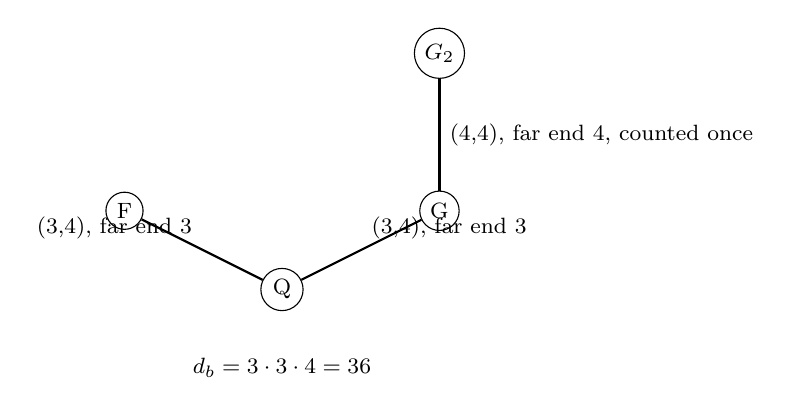
\begin{tikzpicture}[every node/.style={font=\footnotesize}]
\node[circle,draw,inner sep=2pt] (Q) at (0,0) {Q};
\node[circle,draw,inner sep=2pt] (F) at (-2,1) {F};
\node[circle,draw,inner sep=2pt] (G) at (2,1) {G};
\node[circle,draw,inner sep=2pt] (G2) at (2,3) {$G_2$};
\draw[thick] (Q) -- node[above left] {(3,4), far end 3} (F);
\draw[thick] (Q) -- node[above right] {(3,4), far end 3} (G);
\draw[thick] (G) -- node[right] {(4,4), far end 4, counted once} (G2);
\node at (0,-1) {$d_b=3\cdot 3\cdot 4=36$};
\end{tikzpicture}
\caption{The hubs and in-legs of the bottom quark body. The qutrit Q, the hubs F and G at the two (3,4) in-legs and the hub $G_2$ at the one (4,4) hub-to-hub in-leg, whose far-end dimensions multiply to the dressing thirty-six. The out-legs and docks of the body are not drawn.}
\end{figure}
\par\medskip\noindent{\itshape Mass read, Part XI turns to the Higgs.}\label{narr:close:8-5}\par
\section{The Yukawa as the (3,4)-leg office at every body}\label{mod:VI-7a-D541324-w-yklo}
\chdesig{10-6}{6-7a}{VI-7a-D541324-w-yklo}{VI-7a-D541324-w-yklo}
\begin{chwall}[The Yukawa as the (3,4)-leg office at every body]\label{box:VI-7a-D541324-w-yklo:1}
No one per-leg cell among the leg unit, the free-genre first power, the dressing base and their squares factors the offices as the vacuum register multiplied by the cell to the unpassed (3,4) in-leg count: the first parting body is the electron at the count zero at every candidate, its office over the register an element of the field with root parts against the cell one, the equal count zero of 2847 at every candidate, the chain ratios re-met at the neutron over the proton alone, nine at the exponent difference one, the dressing base squared; the top Yukawa cell of the Higgs-and-carrier-offices entry is re-met as the proton office over the register $101761/81$ with the implied per-leg cell $319/9$ at the count two, the hadron cap over the dressing base squared, a per-body cell and no one cell across the bodies; an open result of the factoring at the (3,4) legs under the axiom text, compared with nothing.
The first face, one per-leg cell at every body with the chain re-met, reads unmet; the second face, the first parting body named with both cells, reads yes at the electron, its office over the register against the cell one. Open is the Yukawa as one cell at the (3,4) legs: the top cell of the foregoing entry stands at one body, and a per-leg cell factors no other office.
\end{chwall}
\chstanding{an open result}
\chdeps{Definitions 1.1 to 1.6}{no theorem beyond it at this release}
The top Yukawa of the Higgs-and-carrier-offices entry is the office of one body over the vacuum register at the hub. The question is whether that cell generalizes: whether every office of the five bodies and the 2842 carrier bodies equals the vacuum register multiplied by one fixed per-leg cell raised to the number of (3,4) in-legs its passage leaves unpassed. Six candidates for the cell are read from the entries, the leg unit twelve, the free-genre first power twelve, the dressing base three and their squares, and the vacuum register at its six readings. The electron parts first: its passage passes its one in-leg, so its count is zero and the candidate to the zeroth power is one, while its office over the register carries root parts; at the proton the ratio is the square of $319/9$, a cell of the proton alone. No candidate meets any body, and only the neutron over the proton re-meets a chain ratio.
\begin{chbridge}
In the Standard Model the mass of each fermion is its Yukawa coupling multiplied by the vacuum expectation value of the Higgs field divided by root two, one coupling per body and no relation among them, the top coupling near unity and the others small \cite{Weinberg1967,Peskin1995}. The correspondence is by name.
\end{chbridge}
\begin{chproof}[exhaustive census with its exact part]
The premises of this derivation are the axiom and the six definitions of chapter~\ref{mod:FRAMEWORK}, the body-alone office rule of chapter~\ref{mod:VIII-2-body-alone-office-rule}, a theorem, the dressing as the unpassed (3,4) in-legs of chapter~\ref{mod:VIII-1-mass-unit-and-the-first-power}, a theorem, the Higgs and carrier offices at their sinks of chapter~\ref{mod:VI-10-higgs-the-closed-hub-read-its-rows-its-mass-and-its-exponent}, a theorem, and the vacuum register of the chapter titled The electroweak table (chapter~\ref{mod:VI-9-electroweak-table}, among the instruments), an instrument. The chain of premises runs back to the axiom through those chapters, and the longest such chain in this compendium is twelve chapters long.
\textit{The exact part.} For each body the passage is walked as the unpassed-in-legs entry walks it, the entry at the pendant qubit of the first dock-set link in link order, the stop at the first-reached hubs, every in-leg dressed at a tie and the base the far-end dimension, giving the count $k$ of unpassed (3,4) in-legs, zero at the electron, two at the muon and the proton, three at the tau sink. The six candidates $c$ are 12, 12, 3, 144, 144 and 9, and the vacuum register $R$ is 6561 at its first reading. At the proton,
\begin{equation} \frac{\Omega_{P}}{R} = \frac{101761}{81} = \Big(\frac{319}{9}\Big)^{2}, \qquad c^{2} \in \{144,\ 144,\ 9,\ 20736,\ 20736,\ 81\}, \end{equation}
so the ratio is an exact square whose root $319/9$, the hadron cap over the dressing base squared, equals none of the candidates squared, and the top Yukawa cell is re-met as a cell of the proton alone. At the electron the count is zero and every candidate to the zeroth power is one, while
\begin{equation} \frac{\Omega_{E}}{R} \ \text{carries nonzero root-two and root-three coordinates,} \qquad \frac{\Omega_{E}}{R} \neq 1 , \end{equation}
the four coordinates printed at the table of the entry, so the electron parts at every candidate and is the first parting body. The figure draws the electron web with its passed in-leg.
\textit{The census.} By exhaustive enumeration of the 2847 bodies, the five bodies and the 2842 carrier bodies, with the tau web of the library and the one-link electron web beside: each body is located and walked, 2847 of 2847, the walk re-met against the unpassed-in-legs entry at every cell of the five bodies and the tau sink and against the sinks table of the carrier-bodies entry at every cell of the 2842; the property tested at each body and candidate is whether the residual, the office over the register multiplied by the candidate to the count, is an exact element of the field and whether it equals one; the counts are the residuals exact at 17094 of 17094, the two-read identity holding at every residual, and the letter equal at zero of 2847 bodies at every candidate, the closing candidates none; the chain ratios of the mass-ratios entry are re-met as ratios of the cells at one pair and one candidate alone, the neutron over the proton at nine, the dressing base squared at the exponent difference one. The smallest case is the electron worked above.
\textit{The check.} The counter-tests alter the construction singly and read what moves. Striking the vacuum register moves every residual. Striking the passage moves the electron from the count zero. Striking the square moves the proton residual. Striking the text unmeets the gate. Striking the closure moves the electron residual with the proton and the neutron at a closure of zero unmoved. Each alteration moves the cells it names, five of five. The result was reproduced by an independent route, two engines built apart, the python route against the ruby route, equal at every cell, with the sixteen controls the same.
\chcert{2847}
\begin{figure}[h]\centering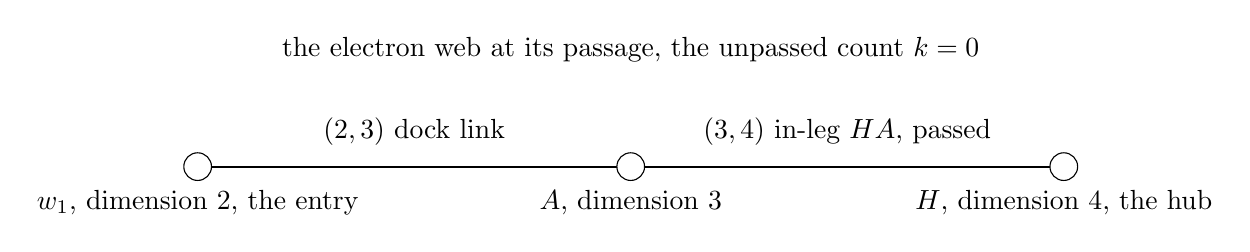
\begin{tikzpicture}[scale=1]
\draw[thick] (0,0) -- (5.5,0); \draw[thick] (5.5,0) -- (11,0);
\filldraw[fill=white] (0,0) circle (5pt) node[below=5pt] {$w_1$, dimension 2, the entry};
\filldraw[fill=white] (5.5,0) circle (5pt) node[below=5pt] {$A$, dimension 3};
\filldraw[fill=white] (11,0) circle (5pt) node[below=5pt] {$H$, dimension 4, the hub};
\node at (2.75,0) [above=4pt] {$(2,3)$ dock link}; \node at (8.25,0) [above=4pt] {$(3,4)$ in-leg $HA$, passed};
\node at (5.5,1) [above=6pt] {the electron web at its passage, the unpassed count $k = 0$};
\end{tikzpicture}\caption{The passage of the electron web: entered at the pendant qubit of its dock link, it reaches the hub through its one (3,4) in-leg, which is therefore passed, so the unpassed count is zero and the first parting stands here.}\end{figure}
\end{chproof}
